\documentclass[11pt,a4paper]{ivoa}
\input tthdefs

\title{VOResource: an XML Encoding Schema for Resource Metadata}

\ivoagroup{Registry}

\author[http://www.ivoa.net/twiki/bin/view/IVOA/RayPlante]{Raymond Plante}
\author[http://www.ivoa.net/twiki/bin/view/IVOA/KevinBenson]{Kevin Benson}
\author[http://www.ivoa.net/twiki/bin/view/IVOA/MarkusDemleitner]{Markus Demleitner}
\author[http://www.ivoa.net/twiki/bin/view/IVOA/MatthewGraham]{Matthew Graham}
\author[http://www.ivoa.net/twiki/bin/view/IVOA/GretchenGreene]{Gretchen Greene}
\author[http://www.ivoa.net/twiki/bin/view/IVOA/PaulHarrison]{Paul Harrison}
\author[http://www.ivoa.net/twiki/bin/view/IVOA/GerardLemson]{Gerard Lemson}
\author[http://www.ivoa.net/twiki/bin/view/IVOA/TonyLinde]{Tony Linde}
\author[http://www.ivoa.net/twiki/bin/view/IVOA/GuyRixon]{Guy Rixon}

\editor{Ray Plante, Markus Demleitner}

\previousversion[http://www.ivoa.net/Documents/REC/ReR/VOResource-20080222.html]{REC -1.03}
\previousversion[http://www.ivoa.net/Documents/WD/ReR/VOResource-20061107.html]
  {WD 2006-11-07}
\previousversion[http://www.ivoa.net/Documents/WD/ReR/VOResource-20060620.html]
  {WD 2006-06-20}
\previousversion[http://www.ivoa.net/Documents/WD/ReR/VOResource-20060530.html]
  {WD-2006-05-30}
      

\begin{document}
\begin{abstract}
This document describes an XML encoding standard for IVOA Resource
Metadata, referred to as VOResource.  This schema is primarily
intended to support interoperable registries used for discovering
resources; however, any application that needs to describe resources
may use this schema.  In this document, we define the types and
elements that make up the schema as representations of metadata terms
defined in Resource Metadata for the Virtual Observatory
\citep{2007ivoa.spec.0302H}.  We also describe the general model for the
schema and explain how it may be extended to add new metadata terms and
describe more specific types of resources.  
\end{abstract}


\section*{Acknowledgments}

This document has been developed with support from the
National Science Foundation's
Information Technology Research Program under Cooperative Agreement
AST0122449 with The Johns Hopkins University, from the
UK Particle Physics and Astronomy
Research Council (PPARC), and from the
Eurpean Commission's Sixth
Framework Program via the 
Optical Infrared Coordination Network (OPTICON).  Funding for the 2016
update was provided by BMBF grant GAVO-2014, grant number 05A14VHA.

\section*{Conformance-related definitions}

The words ``MUST'', ``SHALL'', ``SHOULD'', ``MAY'', ``RECOMMENDED'', and
``OPTIONAL'' (in upper or lower case) used in this document are to be
interpreted as described in IETF standard RFC2119 \citep{std:RFC2119}.

The \emph{Virtual Observatory (VO)} is a
general term for a collection of federated resources that can be used
to conduct astronomical research, education, and outreach.
The \href{http://www.ivoa.net}{International
Virtual Observatory Alliance (IVOA)} is a global
collaboration of separately funded projects to develop standards and
infrastructure that enable VO applications.


\section{Introduction}



\subsection{Role within the VO Architecture}

\begin{figure}
\centering

% Get the architecture diagram from the TCG chair
% http://wiki.ivoa.net/twiki/bin/view/IVOA/IvoaTCG
% If they give you a PDF, for now dumb it down to a png by
% convert -antialias -density 72x72 archdiag.pdf archdiag.png
% Oh -- Notes don't need this; you'd have to remove archdiag.png
% from FIGURES in the Makefile, too.

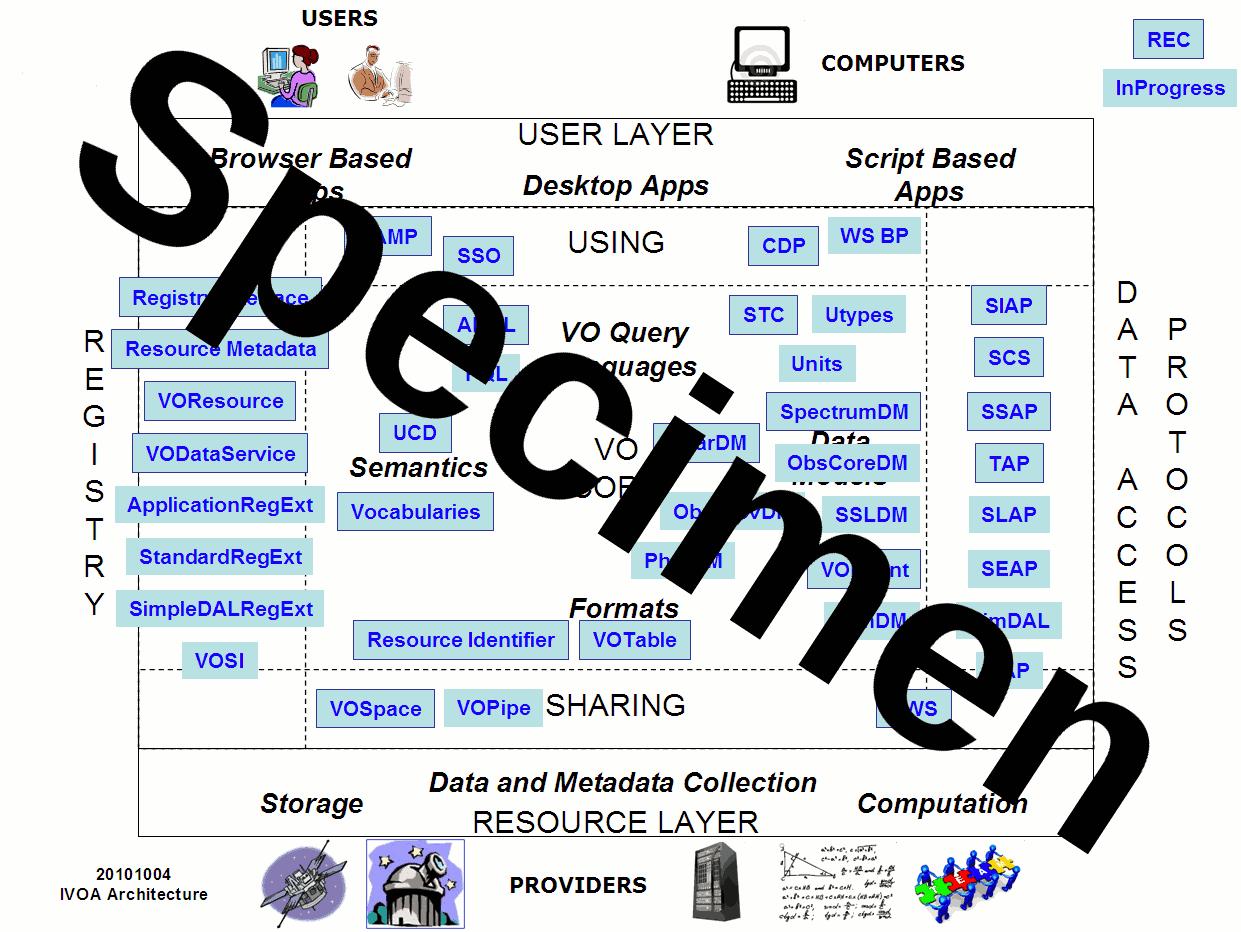
\includegraphics[width=0.9\textwidth]{archdiag.png}
\caption{Architecture diagram for this document}
\label{fig:archdiag}
\end{figure}

Fig.~\ref{fig:archdiag} shows the role this document plays within the
IVOA architecture \citep{note:VOARCH}.

<a name="synnot">
<h3>Syntax Notation Using XML Schema</h3></a>

<p>The eXtensible Markup Language, or XML, is document syntax for marking
textual information with named tags and is defined by the
World Wide Web Consortium (W3C) Recommendation,
<a href="http://www.w3.org/TR/REC-xml">XML 1.0</a>
[<a href="#xml">XML</a>].  The set of XML tag names and the syntax
rules for their use is referred to as the document schema.  One way to
formally define a schema for XML documents is using the W3C standard
known as XML Schema [<a href="#schema">Schema</a>].</p>

<p>
This document defines the VOResource schema using XML Schema.  The
full Schema document is listed in <a href="#appA">Appendix A</a>.
Parts of the schema appear within the main sections of this document;
however, documentation nodes have been left out for the sake of brevity.  
</p>

<p>
Reference to specific elements and types defined in the VOResource
schema include the namespaces prefix, <code>vr</code>, as in
<code>vr:Resource</code> (a type defined in the VOResource schema).
Use of the <code>vr</code> prefix in compliant instance documents is 
not required (see <a href="#ns">section 2.1</a>); its use in this
document is simply to indicate that it is an entity defined in the
VOResource schema.  <!-- References to (local) elements are further
labelled by enclosing the name in the XML tag brackets, as in
<code>&lt;vr:identifier&gt;</code>.  -->
</p>

<h2><a id="contents" name="contents">Contents</a></h2>
<ul class="toc">
  <li><a href="#abstract">Abstract</a></li>
  <li><a href="#status">Status of this document</a></li>
  <li><a href="#acknowledge">Acknowledgments</a></li>
  <li><a href="#conf">Conformance-related definitions</a></li>
  <li><a href="#synnot">Syntax Notation Using XML Schema</a></li>
  <li><a href="#Intro">1. Introduction</a>
  </li><li><a href="#model">2. The VOResource Data Model</a>
       <ul class="toc">
         <li> <a href="#ns">2.1. The Schema Namespace and Location</a>
         </li><li> <a href="#core">2.2. The Core Structural and Semantic Model</a>
         </li><li> <a href="#extend">2.3. Extending the VOResource Schema</a>
       </li></ul>
  </li><li><a href="#metadata">3. The VOResource Metadata</a>
       <ul class="toc">
         <li> <a href="#restype">3.1.  The Base Resource Type</a>
         </li><li> <a href="#resext">3.2.  Resource Type Extensions:  Organisation and Service</a>
       </li></ul>
  </li><li><a href="#appA">Appendix A: the VOResource XML Schema</a></li>
  <li><a href="#appB">Appendix B: Change History</a></li>
  <li><a href="#References">References</a></li>
</ul>
<hr>

<h2><a name="Intro">1. Introduction</a></h2>

<p>
<a name="d:RM">The IVOA Standard,
</a><a href="http://www.ivoa.net/Documents/REC/ResMetadata/RM-20040426.htm">
Resource Metadata for the Virtual Observatory</a>
[<a href="#RM">Hanisch et al. 2004</a>] (hereafter referred to as
<strong>RM</strong>) defines metadata terms for describing resources.
The <a href="#RM">RM</a> defines a <a name="d:resource">resource</a> as: 
</p>

<blockquote>
... VO element that can be described in terms of who curates or
maintains it and which can be given a name and a unique identifier.
Just about anything can be a resource: it can be an abstract idea,
such as sky coverage or an instrumental setup, or it can be fairly
concrete, like an organization or a data collection.  This definition
is consistent with its use in the general Web community as
"anything that has an identity" (Berners-Lee 1998, IETF RFC2396).  We
expand on this definition by saying that it is also describable.  
</blockquote>

<p>
The resource metadata are, then, the terms and concepts that describe
a resource in general.  The RM defines the terms as well as describes
reasonable or allowed values; it does not, however, describe how the
terms and values should be encoded.  This is because resource metadata
may be encoded in several different formats, depending on the
context.  This document specifically describes an encoding called
VOResource.  
</p>

<p>
The primary intended use of VOResource is to provide an XML
interchange format for use with resource registries.  A registry is a
repository of resource descriptions [<a href="#RM">RM</a>] and is
employed by users and applications to discover resources.  VOResource
can be used to pass descriptions from publishers to registries and
then from registries to applications.  Another inended use is as a
language for services to describe themselves directly.  VOResource 
may be used in other ways, in whole or in part, using the standard XML
mechanisms (e.g., import, include).  
</p>

<p>
The VOResource schema provides XML encoding for so-called core
metadata from the <a href="#RM">RM</a> that (with a few exceptions)
can apply to all resources; however, it is recognized that a full and
useful description of a <em>specific</em> resource will require
additional metadata that is relevant only to a resource of its type.
Thus, the VOResource schema has been especially designed to be
extended.  The model for doing this is described in section XX.
</p>

<blockquote>
<table bgcolor="#dddddd" border="2" cellpadding="5"><tbody><tr><td>
<dl>
  <dt> <strong>Note:</strong> </dt>
  <dd> The name "VOResource" has in practice had two meanings within
       IVOA discussions.  The first refers specifically to the core
       XML schema defined by this document.  The second refers more
       broadly to the core schema plus the set of legal extensions.
       In this document, use of the name "VOResource" corresponds to
       the first meaning.  Reference to the broader set of schemas
       will be indicated explicitly with the annotating phrase, "and
       its legal extensions."  </dd>
</dl>
</td></tr></tbody></table>
</blockquote>

<h2><a name="model">2. The VOResource Data Model</a></h2>

<p>
The primary use for VOResource, of course, is to describe a resource
using the metadata concepts defined in the <a href="#RM">RM</a>.  
Here's an example of a VOResource document describing an organisation,
the Radio Astronomy Imaging Group at the National Center for
Supercomputing Applications.  
</p>

<div class="exampleOuter">
<a name="organisation.xml">
</a><div class="exampleHeader"><a name="organisation.xml">Example</a></div>
<div class="exampleWrapper"><a name="organisation.xml">A description of an organisation as a
resource, </a><a href="http://www.ivoa.net/Documents/WD/ReR/organisation.xml">organisation.xml</a></div>
<div class="exampleInner">
<table border="0" cellpadding="0" cellspacing="0"><tbody><tr><td>
<pre>

<font color="red">2</font> 
<font color="purple">1</font>

<font color="blue">3
3</font>

<font color="brown">4
4
4
4
4
<font color="#d00000">5
5
5</font>
<font color="#000090">6
6
6
6
6
6</font>
4
4
4
4
4
4
4
4
4
4
4
4
4
4
4
4
4
4
4
4
4
4
4
4</font>

<font color="green">7
7
7
7</font>


</pre></td><td bgcolor="#d5dee3" width="100%">
<pre>&lt;?xml version="1.0" encoding="UTF-8"?&gt;
&lt;resource <font color="red">xsi:type="Organisation"</font>
  <font color="purple">xmlns:vr="http://www.ivoa.net/xml/VOResource/v1.0"</font>
  xmlns:xsi="http://www.w3.org/2001/XMLSchema-instance"
  <font color="blue">xsi:schemaLocation="http://www.ivoa.net/xml/VOResource/v1.0
                      http://www.ivoa.net/xml/VOResource/v1.0"&gt;</font>

    <font color="brown">&lt;title&gt;NCSA Radio Astronomy Imaging&lt;/title&gt;
    &lt;shortName&gt;NCSA-RAI&lt;/shortName&gt;
    &lt;identifier&gt;ivo://rai.ncsa/RAI&lt;/identifier&gt;

    &lt;curation&gt;
      <font color="#d00000">&lt;publisher ivo-id="ivo://ncsa.uiuc/NCSA"&gt;
         National Center for Supercomputing Applications
      &lt;/publisher&gt;</font>
      <font color="#000090">&lt;creator&gt;
        &lt;name&gt;   Dr. Richard Crutcher    &lt;/name&gt;
        &lt;logo&gt;
           http://rai.ncsa.uiuc.edu/rai.jpg
        &lt;/logo&gt;
      &lt;/creator&gt;</font>
      &lt;date&gt;1993-01-01&lt;/date&gt;
      &lt;contact&gt;
        &lt;name&gt;Dr. Raymond Plante&lt;/name&gt;
	&lt;email&gt;rplante@ncsa.uiuc.edu&lt;/email&gt;
      &lt;/contact&gt;
    &lt;/curation&gt;

    &lt;content&gt;
      &lt;subject&gt;radio astronomy&lt;/subject&gt;
      &lt;subject&gt;data repositories&lt;/subject&gt;
      &lt;subject&gt;digital libraries&lt;/subject&gt;
      &lt;subject&gt;grid-based processing&lt;/subject&gt;
      &lt;description&gt;
        The Radio Astronomy Imaging Group at the National Center for
        Supercomputing Applications is focused on applying
        high-performance computing to astronomical research.  Our
        projects include the NCSA Astronomy Digital Image Library, 
        the BIMA Data Archive, the BIMA Image Pipeline, and the
        National Virtual Observatory. 
      &lt;/description&gt;
      &lt;referenceURL&gt;http://rai.ncsa.uiuc.edu/&lt;/referenceURL&gt;
      &lt;type&gt;Organisation&lt;/type&gt;
      &lt;contentLevel&gt;Research&lt;/contentLevel&gt;
    &lt;/content&gt;</font>

    <font color="green">&lt;facility&gt;Berkeley-Illinois-Maryland Array (BIMA)&lt;/facility&gt;
    &lt;facility&gt;
       Combined Array for Research in Millimeter Astronomy (CARMA)
    &lt;/facility&gt;</font>

&lt;/resource&gt;
</pre></td></tr></tbody></table>
</div></div>

<p>
This example illustrates some important components of a VOResource
record:
</p>
<ol>
  <li> <font color="purple">the VOResource namespace, </font> </li>
  <li> <font color="red">the specific type of resource indicated by
       the value of the <code>xsi:type</code> attribute, </font></li>
  <li> <font color="blue">the location of the schema documents used by
       this description, </font> </li>
  <li> <font color="brown">values for the three main types core metadata:
       identity, curation, and content, </font></li>
  <li> <font color="#d00000">a reference to another resource is made by
       providing that resource's IVOA identifier,</font></li>
  <li> <font color="#000090">string values can be padded with spaces
       for easier readability,</font></li>
  <li> <font color="green">extension metadata specific to the type of
       resource.</font> 
</li></ol>

<h3><a name="ns">2.1. The Schema Namespace and Location</a></h3>

<p>
The VOResource schema namespace is "http://www.ivoa.net/xml/VOResource/v1.0".
The namespace URI has been chosen to allow it to be resolved as a URL
to the XML Schema document (given in <a href="#appA">Appendix A</a>)
that defines the VOResource schema.  Applications may assume that the 
namespace URI is so resolvable.
</p>

<p>
Authors of instance documents that use the VOResource schema may choose to
provide a location for VOResource XML Schema document using the
<a href="http://www.w3.org/TR/xmlschema-0/#schemaLocation">
<code>xsi:schemaLocation</code></a> attribute; the choice of
the location value is the choice of the author.  In general, the use
of <a href="http://www.w3.org/TR/xmlschema-0/#schemaLocation">
<code>xsi:schemaLocation</code></a> is recommended by
this specification with a the namespace URI given as the location as
illustrated in the example above, unless the application prefers
otherwise.
</p>

<blockquote>
<pre>xsi:schemaLocation="http://www.ivoa.net/xml/VOResource/v1.0
                    http://www.ivoa.net/xml/VOResource/v1.0"</pre>
</blockquote>

<p>
Whenever instance <a href="#d:valid">validation</a> is needed, use of
the VOResource schema and its legal extensions must be declared using
the standard namespace declaration attribute, 
<code>xmlns:<i>prefix</i></code> (where <i>prefix</i> is an arbitrary
prefix).  The prefix, <code>vr</code>, is used by convention as the
prefix defined for the VOResource schema; however, instance documents
may use any prefix of the author's choosing.  In this document, the
<code>vr</code> prefix is used to label, as shorthand, a type or
element name that is defined in the VOResource schema, as in
<code>vr:Resource</code>. 
</p>

<p>
Because the VOResource XML schema sets
<code>elementFormDefault="unqualified"</code>, documents that use the
VOResource schema should not use the namespace declaration attribute,
<code>xmlns</code> (used to set the default namespace), anywhere in
the document where the VOResource schema is in effect.  (This is a
restriction set by the rules of XML Schema.)  Furthermore, in
accordance with the Schema rules for unqualified elements, the
VOResource namespace prefix must not used to qualify VOResource
elements.  In general, namespace prefixes are only used to qualify
type names given as values to the <code>xsi:type</code> attribute (see
next section).  Legal extensions of the VOResource schema SHOULD also
set <code>elementFormDefault="unqualified"</code> for consistancy.
</p>

<a name="core">
<h3>2.2. The Core Structural and Semantic Model</h3></a>

<p>
The VOResource schema only defines global types; it does not define
any global elements (often refered to as root elements).  It is the
responsibility of the application to define the root element of the
VOResource-employing documents it operates on.  Typically, the root
element is defined in a separate application-specific schema.  The
type of an application document's root element is not assumed to be
any particular type defined in the VOResource schema (nor any of its
legal extensions).  In fact, it need not be of a type from the
VOResource at all; rather, VOResource types may appear anywhere in the
document.   
</p>

<p>
</p><blockquote>
<table bgcolor="#dddddd" border="2" cellpadding="5"><tbody><tr><td>
<dl>
  <dt> <strong>Note:</strong> </dt>
  <dd> The IVOA Registry Interface standard, for example, includes a
       small schema that defines a single global element,
       <code>&lt;VOResources&gt;</code>, that can contain a series of
       <code>&lt;resource&gt;</code> child elements.  The child
       element is defined to be of the type <code>Resource</code> from
       the VOResource schema.  </dd>
</dl>
</td></tr></tbody></table>
</blockquote>
<p></p>

<p>
</p><blockquote>
<table bgcolor="#dddddd" border="2" cellpadding="5"><tbody><tr><td>
<dl>
  <dt> <strong>Note:</strong> </dt>
  <dd> In the <a href="#organisation.xml">example instance
       document</a> at the beginning of section 2, the root element,
       <code>&lt;resource&gt;</code> is not defined in any schema.
       Nevertheless, this document is still legal and verifiable XML.
       This is because the element's type is explicitly specified with
       the <code>xsi:type</code> attribute.  </dd>
</dl>
</td></tr></tbody></table>
</blockquote>
<p></p>

<p>
<a name="nameconv">VOResource uses the following conventions for
names of elements and types:
</a></p><ul>
<a name="nameconv">  <li> all global types it defines have names that are capitalized.
       (This practice would extend to global elements, if they existed
       in the VOResource.)   </li>
  <li> Locally defined elements begin with a lower-case character. </li>
  <li> For all types and element names that are made up of multiple
       words, such as <code>shortName</code>, upper-case letters are
       used demarcate the start of appended word (the "camel"
       format).  </li>
  <li> Names that include abbreviations, such as
       <code>IdentifierURI</code>, all letters in the abbreviation are
       capitalized.  </li>
</a></ul>
<a name="nameconv">It is recommended that this convention be followed in other schemas
that either use the VOResource schema (via an <code>xsd:import</code> or
<code>xsd:include</code>) or extend it.  
</a><p></p>

<p>
<a name="nameconv">Applications describe a single resource using an element of the type
<code>vr:Resource</code> or a legal derivation of it.
</a><a name="d:core">The content of the <code>vr:Resource</code> type is
referred to as the <strong>core VOResource metadata</strong></a>, and
they fall into four categories (corresponding to the sections 3.1,
3.2, 3.3, and 4 of the RM):

</p><ul>
  <li> identity metadata:  the <code>&lt;title&gt;</code>,
       <code>&lt;shortName&gt;</code>, and
       <code>&lt;identifier&gt;</code> elements;
  </li><li> curation metadata:  the contents of the
       <code>&lt;curation&gt;</code> element;
  </li><li> general content metadata:  the contents of the
       <code>&lt;content&gt;</code> element;
  </li><li> metadata quality flags:  the
       <code>&lt;validationLevel&gt;</code> element.
</li></ul>

<p>
These elements are defined in more detail in <a href="#metadata">section 3.</a>
</p>

<p>
Many of the elements in VOResource that are meant to have string or
URI values are defined as being of the type <code>xs:token</code>.
This allows authors of VOResource instance documents to pad string and
URI values with spaces and include carriage returns to improve
readability.  The definition of these types will cause an XML
Schema-compliant parser to replace tab, line feed, and carraige return
characters with simple spaces, then replace multiple sequential
occurrences of spaces with a single space, and then remove all leading
and trailing spaces.  
</a></p>

<p>
<a name="d:UTCDateTime">All VOResource elements and attributes that
contain dates must be interpreted as </a><a href="#d:utc">UTC</a> dates and
must be encoded in compliance with ISO8601 standard Date and Time Format
[<a href="#iso8601">ISO8601</a>].  The <code>vr:UTCTimestamp</code>
type provides a special restriction of the format that requires
includsion of date and time, but disallows the timezone format.  This 
enforces a restricted form of this format which allows encoding of the
date and time, but disallows the timezone format:
</p>

<div class="schemaOuter">
<a name="s:UTCDateTime">
</a><div class="schemaHeader"><a name="s:UTCDateTime">vr:UTCTimestamp Schema Definition</a></div>
<div class="schemaInner">
<pre>&lt;xs:simpleType name="UTCTimestamp"&gt;
   &lt;xs:restriction base="xs:dateTime"&gt;
      &lt;xs:pattern value="\d{4}-\d\d-\d\dT\d\d:\d\d:\d\d(\.\d+)?"/&gt;
   &lt;/xs:restriction&gt;
&lt;/xs:simpleType&gt;
</pre>
</div>
<div class="schemaHeader"><a name="s:UTCDateTime">vr:UTCDateTime Schema Definition</a></div>
<div class="schemaInner">
<pre>&lt;xs:simpleType name="UTCDateTime"&gt;
   &lt;xs:union memberTypes="xs:date vr:UTCTimestamp"/&gt;
&lt;/xs:simpleType&gt;
</pre>
</div></div>

<p>
<a name="d:UTCDateTime">The <code>vr:UTCDateTime</code> type allows the date to appear either
as a simple date--i.e. conforming to <code>xs:date</code>--or as a
date and time as restricted by <code>vr:UTCTimestamp</code>.  
When either of these VOResource types is used, authors must provide an
applicable UTC date and time, and applications must interpret the time
and date as UTC. 
</a></p>

<p><a name="doc">
All VOResource types and elements have an associated semantic meaning
which is given in the first <code>&lt;xsd:documentation&gt;</code>
node within the type or element's definition in the schema.  The
meaning associated with a type is generic, indicating the kind of
information the type provides.  The semantics that are delivered by a
VOResource instance document, however, are those associated with
VOResource elements.  The meaning of a VOResource element can be
thought of as having two parts:  the generic meaning of the set of
information it contains as defined by its type, and a specific meaning
describing the context in which that information applies.  Because all
VOResource elements are locally defined (in the XML Schema
sense), they do not have an absolute meaning, but rather have a
meaning tied to the thing being described by that element as
represented by the enclosing type.  
</a></p>

<a name="doc">Here are three examples that illustrate the semantics communicated by
VOResource entities:

</a><ol>
<a name="doc">  <li> <p>The <code>vr:Curation</code> type describes the curation of a
       resource.  The <code>&lt;curation&gt;</code> element
       describes curation of the specific resource described by the
       enclosing <code>vr:Resource</code> type and identified by its
       <code>identifier</code> element. </p></li>

  <li> <p>The <code>vr:ResourceName</code> type is a generic reference to
       another resource.  The <code>&lt;publisher&gt;</code> element
       gives a reference to the publisher of the specific resource being
       described which may itself be a registered resource described
       elsewhere.  </p></li>

  <li> <p>The <code>&lt;title&gt;</code> element gives the title of
       the resource being described the enclosing
       <code>vr:Resource</code> type and identified by its
       <code>&lt;identifier&gt;</code> element.  The
       <code>&lt;title&gt;</code> element's type,
       <code>xs:token</code> (a restriction on
       <code>xsd:string</code>), has no inherent meaning associated
       with it.  </p></li> 
</a></ol>

<p>
<a name="doc">Additional semantics are transmitted through the use of derived types
using the <code>xsi:type</code> attribute.  In the
</a><a href="#organisation.xml">sample instance document</a> above, the
use of <code>xsi:type="Organisation"</code> means that the resource
being described is specifically an organisation as defined by the
<code>vr:Organisation</code> type.  This type provides additional
metadata that are not part of the core resource metadata.  The
semantics associated with the use of <code>xsi:type</code> is
described further in the <a href="#xsitype">next subsection</a>.
</p>

<a name="xsitype">
<h4>2.2.1.  Refined Semantics with Derived Types</h4></a>

<p>
When a resource is described with an element explicitly of the type
<code>vr:Resource</code>, it is being described in the most generic
sense.  The metadata presented in this type, including both free text
values and controlled vocabulary, can give some sense of what
type of resource is being described and what it might be used for.
However, the most useful descriptions of resources will not explicitly
use the <code>vr:Resource</code> type; rather, they will use types
that are derived from <code>vr:Resource</code>.  
</p>

<p>
Defining derived <code>vr:Resource</code> types accomplishes two
things:
</p><ol>
  <li> it sharpens the semantic meaning of the resource description by
       indicating what specific type of resource it is, and
  </li><li> it <em>may</em> allow additional metadata not part of the core
       but specific to the that type of resource.
</li></ol>
<p></p>

<p>
The VOResource schema defines two types derived from
<code>vr:Resource</code>:  <code>vr:Organisation</code> and
<code>vr:Service</code>.   The <code>vr:Organisation</code> adds
metadata describing the astronomical facilities such as telescopes
that are associated with the organisation it describes.  The
<code>vr:Service</code> type adds an element called
<code>capability</code> which describes the service's interface as
well as information regarding its behavior.  
</p>

<p>
Extensions of the <code>vr:Resource</code> type is a key way
derivation is used in VOResource to provide refined resource
descriptions.  Two other important parent types in the schema are
<code>vr:Capability</code> and <code>vr:Interface</code>; these are
extended to provide more refined descriptions of services (see <a href="#servicemod">section 2.2.2</a>).  The motivation for extending
these types are the same as for <code>vr:Resource</code>: to provide
more specific semantic meaning through the derived type's name, and to
provide additional, specialized metadata that is not part of the
parent type.  Note, however, that in general, a derived type need not
alter the content model of its base type.  This allows derived types
to add more specific meaning with out adding any additional metadata.
</p>

<p>
As described in <a href="#core">section 2.2</a>, it is intended that
derived <code>vr:Resource</code>, <code>vr:Capability</code> and
<code>vr:Interface</code> types be invoked in instance
documents using the <code>xsi:type</code> attribute (as illustrated in
the <a href="#organisation.xml">sample document</a> above).  This
method illustrates a polymorphism for resource metadata in that any
place where an element of parent type is expected, the derived type
may be inserted.  The use of <code>xsi:type</code> illustrates both
what specific type is being inserted in as well as what it is being
inserted in for.  That is, as in our
<a href="#organisation.xml">example</a>, the <em>resource</em> being
described is an <em>organisation</em>.  
</p>

<p>
The other mechanism for polymorphism provided by XML Schema
[<a href="#schema">Schema</a>] is substitution groups.  Invoking
derived <code>vr:Resource</code> types via elements in a substitution
group is discouraged because it is less obvious from looking at the
instance document that a substitution is being made.  
</p>

<a name="servicemod">
<h4>2.2.2 The Service Data Model</h4>
</a>

<p>
The <code>vr:Service</code> type extends the core
<code>vr:Resource</code> metadata data by adding the
<code>capability</code> element (see <a href="#d:Service">section
3.2.2</a>).  This element is used to describe a major functionality of
the service, usually accessible through a single service endpoint URL.
In particular, it is used to describe support for an IVOA service
standard (e.g. Simple Image Access Protocol).  A service resource
record may have multiple child <code>capability</code> elements, each
describing a different major functionality; however, these
capabilities should be related in an obvious, logical way by virtue of
sharing same <a href="#d:core">core VOResource metadata</a>.  
</p>

<blockquote>
<table bgcolor="#dddddd" border="2" cellpadding="5"><tbody><tr><td>
<dl>
  <dt> <strong>Note:</strong> </dt>
  <dd> Whether multiple related capabilities are grouped together in a
       single Service record or are described in separate Service
       records is expected to be the choice of the VOResource record
       author.  However, it is also expected that resource registry
       providers will provide some guidance to authors on best
       practices.  This guidance could in part come in the form of a
       GUI that naturally encourage or contrains to aggregation of
       capabilities in a single record.  </dd>
</dl>
</td></tr></tbody></table>
</blockquote>

<p>
The <code>capability</code> element, through its type
<code>vr:Capability</code>, describes the behavior of service
capability and how to access it.  The latter is described by a child
<code>interface</code> element.  As for the behavior, the base
<code>vr:Capability</code> type only provides a
<code>description</code> element that can contain human-readable text
on what this capability provides.  More structured behavioral
information must be provided through specialized
<code>vr:Capability</code> extensions.  In particular, it is expected
that a service standard (e.g. Simple Image Access Protocol) would
define an extension of <code>vr:Capability</code> that adds additional
metadata that can describe the service's behavior in relation to the
standard; for example, the added metadata can describe limitations of
the service implementation or indicate support for optional features.
The specific <code>vr:Capability</code> type is invoked using the
<code>xsi:type</code> mechanism described in
<a href="#xsitype">section 2.2.1</a>.   
</p>

<div class="exampleOuter">
<a name="capability-xsi:type">
</a><div class="exampleHeader"><a name="capability-xsi:type">Example</a></div>
<div class="exampleWrapper"><a name="capability-xsi:type">Invoking a specialized Capability type for
a standard service capability.  In this example, it is assumed that
<code>SimpleImageAccess</code> extension type is defined in a separate
schema document. </a></div>
<div class="exampleInner" style="background-color: rgb(213, 222, 227);">
<pre><a name="capability-xsi:type">&lt;capability xsi:type="sia:SimpleImageAccess"
            standardID="ivo://ivoa.net/std/SIA"&gt;
  ...
&lt;/capability&gt;
</a></pre>
</div></div>

<p>
<a name="capability-xsi:type">As the example above suggests, a common way for locating or otherwise
identifying support for a standard service capability is by looking
for the appropriate value in a <code>capability</code>'s
<code>xsi:type</code> attribute.  
</a></p>

<p>
<a name="capability-xsi:type">If the service capability being described does not conform to any
standard or if the standard does not require any specialized
capability metadata for describing an implementation's behavior, then
no <code>vr:Capability</code> extension is required.  In this case,
the base <code>capability</code> element is simply used without any
<code>xsi:type</code> attribute provided.  It is expected that the
metadata provided outside of the <code>capability</code> element as
well as (optionally) it's <code>description</code> element is
sufficient for describing what the service does.  
</a></p>

<p>
<a name="capability-xsi:type">Because each <code>vr:Capability</code> extension features a different
set of behavioral metadata, introducing a new
<code>vr:Capability</code> extension can impose a non-trivial cost on
applications that process VOResource records.  Thus, an alternative
way to indicate support for a service standard is provided by the
<code>standardID</code> attribute which is useful when the standard
does not require any specialized behavioral metadata to be provided.
The value is set to a URI which represents the service standard.  Some
service standards that do extend <code>vr:Capability</code>
<em>may</em> force the value of this attribute to be set to the
appropriate value (see </a><a href="#extendService">section 2.3.2</a>);
this allows one to use, when appropriate, the <code>standardID</code>
as a way to locate support for a standard regardless of whether an
extension type has been defined or not.   
</p>

<p>
Each <code>capability</code> element can contain one or more child
<code>interface</code> elements, each describing how the capability
can be accessed.  The <code>interface</code> element's type,
<code>vr:Interface</code>, is abstract; thus, the
<code>interface</code> element must be accompanied by an
<code>xsi:type</code> attribute that indicates an
<code>vr:Interface</code> extension type.  The VOResource schema
defines two <code>vr:Interface</code> extension types:
<code>vr:WebBrowser</code>, for describing an interface access via web
browser, and <code>vr:WebService</code>, for accessing a service
described by a Web Service Description Language (WSDL) document (see
section XX for details).  
</p>

<div class="exampleOuter">
<a name="capability-xsi:type">
</a><div class="exampleHeader"><a name="capability-xsi:type">Example</a></div>
<div class="exampleWrapper"><a name="capability-xsi:type">Describing a typical SOAP-based Web
Service interface. </a></div>
<div class="exampleInner" style="background-color: rgb(213, 222, 227);">
<pre><a name="capability-xsi:type">&lt;interface xsi:type="vr:WebService"&gt;
   &lt;accessURL&gt; http://archive.org/service/query &lt;/accessURL&gt;
&lt;/capability&gt;
</a></pre>
</div></div>

<p>
<a name="capability-xsi:type">When a <code>capability</code> contains more than one
<code>interface</code>, each <code>interface</code> should be
interpreted as an alternative interface for accessing essentially the
same underlying capability.  The interfaces can differ in their
overall type (e.g. <code>vr:WebBrowser</code>,
<code>vr:WebService</code>) or in the supported input parameters or
output products.  
</a></p>

<p>
<a name="capability-xsi:type">When a standard capability is being described (i.e. either the
<code>vr:Capability</code> sub-type is defined by a standard or the
<code>standardID</code> is provided), then at least one of the
<code>interface</code> elements should describe an interface required
by the standard.  The <code>role</code> attribute is used to mark the
standard interfaces (typically with the value "std"; see section XX
for details).  All other interfaces are considered non-standard
alternatives.
</a></p>

<p>
<a name="capability-xsi:type">Another important way <code>interface</code>s inside the same
<code>capability</code> element can be different is in the version of
the service standard the interface supports.  Whenever, an interface
supports a version other than "1.0", the <code>interface</code>
element must include a <code>version</code> attribute set to the
version being supported.  Valid values for <code>version</code> are
defined by the standard.  
</a></p>

<div class="exampleOuter">
<a name="capability-xsi:type">
</a><div class="exampleHeader"><a name="capability-xsi:type">Example</a></div>
<div class="exampleWrapper"><a name="capability-xsi:type">Describing multiple interfaces for the
same capability.  In this example, it is assumed that
<code>SkyNode</code> extension type is defined in a separate
schema document. </a></div>
<div class="exampleInner" style="background-color: rgb(213, 222, 227);">
<pre><a name="capability-xsi:type">&lt;capability xsi:type="sn:SkyNode"
            standardID="ivo://ivoa.net/std/SkyNode"&gt;

  &lt;!--  version 1.0 of the standard SkyNode interface --&gt; 
  &lt;interface xsi:type="vr:WebService" role="std" version="1.0"&gt;
     &lt;accessURL&gt; http://archive.org/service/skynode &lt;/accessURL&gt;
  &lt;/interface&gt;

  &lt;!--  version 1.1 of the standard SkyNode interface --&gt; 
  &lt;interface xsi:type="vr:WebService" role="std" version="1.1"&gt;
     &lt;accessURL&gt; http://archive.org/service/skynode1.1 &lt;/accessURL&gt;
  &lt;/interface&gt;

  &lt;!--  a interactive alternative interface, assesible via a browser  --&gt; 
  &lt;interface xsi:type="vr:WebBrowser"&gt;
     &lt;accessURL&gt; http://archive.org/skynode.html &lt;/accessURL&gt;
  &lt;/interface&gt;
  ...
&lt;/capability&gt;
</a></pre>
</div></div>

<!--
<a name="validationLevel">
<h4>2.2.3.  Tagging Metadata Quality</h4></a>

VOResource uses elements called <code>validationLevel</code> to encode
the <em>ResourceValidationLevel</em> metadatum as defined in the
<a href="#d:RM">RM</a>; it is defined as:

<blockquote>
A numeric grade describing the quality of the resource description and
interface, when applicable, to be used to indicate the confidence an
end-user can put in the resource as part of a VO application or
research study. 
</blockquote>
-->

<a name="extend">
<h3>2.3. Extending the VOResource Schema</h3></a>

<p>
A schema made up only of global type definitions provides great
flexibility for extension.  Any global type defined in the VOResource
schema may be used as the base of a derived type defined in another
schema.  The schema containing the derived types must declare its own
namespace URI or default to the null namespace; it must not adopt the
<a href="#ns">VOResource namespace URI</a>.  The application must then
define what schemas, identified by their namespace URIs, are supported
and/or required.  
</p>

<p>
A <a name="d:extend"><strong>VOResource extension</strong></a> is an
XML Schema document whose primary purpose is to define new types
derived from those defined in the VOResource schema for use in
resource descriptions.  It is recommended that VOResource extensions
follow the definition styles used by the core VOResource.  In
particular: 
</p><ul>
  <li> <p><em>Provide semantic definitions of all types and elements within
       the first <code>&lt;xsd:documentation&gt;</code> element inside
       the type or element definition.</em>  Subsequent
       <code>&lt;xsd:documentation&gt;</code> elements may provide
       additional comments or discussion.</p>  </li>

  <li> <p><em>Avoid the use of <code>xsd:choice</code> elements.</em>
       VOResource does not use the choice structure because it does
       not map readily into any object-oriented software language
       structure.  Choices are handled instead as multiple derived
       types that can be inserted in place of a parent type.</p>  </li>

  <li> <p><em>Avoid the use of substitution groups</em>.  VOResource
       prefers instead the use of <code>xsi:type</code> which are
       (with a few exceptions) functionally equivalent to substitution
       groups in terms of structure; however, <code>xsi:type</code>
       serves as an obvious flag in the instance document that a
       substitution has been made.</p> </li>

  <li> <p><em>Choose semantically meaningful names for derived
       types.</em>  When the derived type appears in the pattern
       <code>&lt;<i>elname</i> xsi:type="<i>derivedType</i>"&gt;</code>, 
       choose a <i>derivedType</i> name such that the sentence, "a
       <i>derivedType</i> is a kind of <i>elname</i>" makes natural
       and obvious sense.  For example, "an <i>Organisation</i> is a
       kind of <i>resource</i>."</p> </li>

  <li> <p><em>Follow the VOResource naming conventions</em>.</p> </li>
</ul>
<p></p>

<p>
There are two types of derivation that are particularly important to
the VOResource data model:  derivation of the <code>vr:Resource</code>
type, used to define specific types of resources, and the derivation
of service metadata elements.  
</p>

<a name="extendResource">
<h4>2.3.1.  Defining New Resource Types</h4>
</a>

<!--
<p>
<blockquote>
<table cellpadding="5" bgcolor="#dddddd" border="2"><tbody><tr><td>
<dl>
  <dt> <strong>Note:</strong> </dt>
  <dd> It is recommended that the IVOA standards document that defines
       an IVOA standard service should include the definition of a
       VOResource extension schema that is used to describe
       implementations of the service in a registry.  This schema
       would include a type that derives from <code>vr:Service</code>
       and may also include extensions of <code>vr:Interface</code>
       and/or <code>vr:Capability</code> (see sections
       <a href="#extendService">2.3.2</a> and
       <a href="#d:Service">3.2.2</a>).  </dd>
</dl>
</td></tr></tbody></table>
</blockquote>
</p>
-->

<p>
Derivation of <code>vr:Resource</code> to define new kinds of
resources should be done by extension (i.e. using 
<code>&lt;xsd:extension&gt;</code>) rather than restriction.  It is
not required that the derived type change the content model from that
of the <code>vr:Resource</code> base type; in this case, the purpose
of the derivation is only to sharpen the semantic meaning of the
resource description.  
</p>

<a name="extendService">
<h4>2.3.2.  Defining New Service Capabilities and Interfaces </h4></a>

<p>
As described in <a href="#servicemod">section 2.2.3</a>, a service
standard will often define a new <code>vr:Capability</code> extension
type to allow implementations to describe how they support the
standard.  This definition of the <code>vr:Capability</code> extension
should be done in a schema document with a namespace identifier that
is dedicated to that standard (hereafter referred to as <em>the
standard's extension schema</em>).  The extension type should include
elements representing the applicable Capability metadata described in
section 5.2 of the <a href="#d:RM">RM</a>
(e.g. <em>Service.MaxReturnRecords</em>, <em>Service.MaxReturnSize</em>)
but can also include other concepts that are specific to that standard.
</p>

<p>
The standard's extension schema <em>may</em> create a derived
<code>vr:Capability</code> type that forces the value of the
<code>standardID</code> attribute to be set to a given URI.  This
should be done by first deriving from <code>vr:Capability</code> by
<em>restriction</em> (i.e. using
<code>&lt;xsd:restriction&gt;</code>), keeping all of the parent's
content model except adding to the <code>standardID</code>'s attribute
definition <code>use="required"</code> along with the
<code>fixed</code> modifier set to the desired URI.  Since this
restricted type is not intended for direct use in an instance
document, it should be marked as abstract.  The restricted type should
then be extended to add the specialized capability metadata required
by the standard.  (See the example below.)  
</p>

<p>
It is not recommended that standard's extension schema attempt to
force the inclusion of a required interface type.  
</p>

<p>
An extension schema can define new interface types, though not
necessarily in the context of any specific standard service
capability.  The basic <code>vr:Interface</code> type provides only
<code>accessURL</code> and <code>securityMethod</code> as child
elements.  A derived <code>vr:Interface</code> type must indicate in
the documentation how the <code>&lt;accessURL&gt;</code> should be
interpreted and used.  The derived type may also include other added
metadata describing how to use the service (e.g., a description of the
input arguments).  If the interface extension type is expected to be
referenced by a standard service capability, then it is recommended
that the additional metadata be optional unless the metadata is
absolutely required by clients in order to invoke the service.
</p>

<p>
</p><blockquote>
<table bgcolor="#dddddd" border="2" cellpadding="5"><tbody><tr><td>
<dl>
  <dt> <strong>Note:</strong> </dt>
  <dd> It is intended that a set of common generic interface types
       would be defined in a separate VOResource extension schema.
       At the time of this writing, this schema is called
       VODataService.  It currently defines an interface type for
       describing traditional GET and POST services.  More specific
       interfaces, particularly those associated with standard IVOA
       services (like a Registry Service) would derive its specific
       interface descriptions from one of the common types as
       appropriate.  </dd> 
</dl>
</td></tr></tbody></table>
</blockquote>
<p></p>

<p>
</p><blockquote>
<table bgcolor="#dddddd" border="2" cellpadding="5"><tbody><tr><td>
<dl>
  <dt> <strong>Note:</strong> </dt>
  <dd> The Simple Image Access Protocol [<a href="#sia">SIA</a>] is an
       example of a standard service that defines capability
       metadata.  These include "maxRecords" that list the maximum
       number of records the SIA implementation can return at a time,
       and "MaxImageSize" gives the maximum image size that the
       service can return.  </dd>
</dl>
</td></tr></tbody></table>
</blockquote>
<p></p>

<div class="exampleOuter">
<div class="exampleHeader">Example</div>
<div class="exampleWrapper">How a Capability element can be defined to
describe the Simple Image Access Protocol...</div>
<div class="exampleInner" style="background-color: rgb(213, 222, 227);">
<pre>&lt;?xml version="1.0" encoding="UTF-8"?&gt;
&lt;xs:schema xmlns:xs="http://www.w3.org/2001/XMLSchema" 
           xmlns:vr="http://www.ivoa.net/xml/VOResource/v1.0"
           xmlns:vs="http://www.ivoa.net/xml/VODataService/v1.0"
           xmlns:sia="http://www.ivoa.net/xml/SIA/v1.0"
           targetNamespace="http://www.ivoa.net/xml/SIA/v1.0"
           elementFormDefault="unqualified" attributeFormDefault="unqualified"
           version="1.0"&gt;

   &lt;xs:annotation&gt;
      &lt;xs:documentation&gt;
        An XML Schema for describing a Simple Image Access Service
        implementation.   
      &lt;/xs:documentation&gt;
   &lt;/xs:annotation&gt;

   &lt;xs:import namespace="http://www.ivoa.net/xml/VOResource/v1.0"/&gt;

   &lt;xs:complexType name="SIACapRestriction" abstract="true"&gt;
      &lt;xs:annotation&gt;
         &lt;xs:documentation&gt;
            an abstract capability that fixes the standardID to the
            URI for the SIA standard.
         &lt;/xs:documentation&gt;
      &lt;/xs:annotation&gt;
      &lt;xs:complexContent&gt;
         &lt;xs:restriction base="vr:Capability"&gt;
            &lt;xs:sequence&gt;
               &lt;xs:element name="validationLevel" type="vr:Validation"
                           minOccurs="0" maxOccurs="unbounded"/&gt;
               &lt;xs:element name="description" type="vr:token" 
                           minOccurs="0"/&gt;
               &lt;xs:element name="interface" type="vr:Interface" 
                           minOccurs="0" maxOccurs="unbounded"/&gt;
            &lt;/xs:sequence&gt;
            &lt;xs:attribute name="standardID" type="vr:IdentifierURI"
                          use="required" fixed="ivo://ivoa.net/std/SIA"/&gt;
         &lt;/xs:restriction&gt;
      &lt;/xs:complexContent&gt;
   &lt;/xs:complexType&gt;

   &lt;xs:complexType name="SimpleImageAccess"&gt;
      &lt;xs:annotation&gt;
         &lt;xs:documentation&gt;
            The behavior and limitations of an SIA implementation.  
         &lt;/xs:documentation&gt;
      &lt;/xs:annotation&gt;

      &lt;xs:complexContent&gt;
         &lt;xs:extension base="sia:SIACapRestriction"&gt;
            &lt;xs:sequence&gt;

               &lt;xs:element name="maxRecords" type="xs:int"&gt;
                  &lt;xs:annotation&gt;
                     &lt;xs:documentation&gt;
                        The largest number of records that the Image Query web
                        method will return. 
                     &lt;/xs:documentation&gt;
                  &lt;/xs:annotation&gt;
               &lt;/xs:element&gt;

               &lt;!-- other capability metadata --&gt;
            &lt;/xs:sequence&gt;
         &lt;/xs:extension&gt;
      &lt;/xs:complexContent&gt;
   &lt;/xs:complexType&gt;

&lt;/xs:schema&gt;
</pre>
</div>
<div class="exampleWrapper">...and what a supporting instance document
would look like. </div>
<div class="exampleInner" style="background-color: rgb(213, 222, 227);">
<pre>&lt;resource xsi:type="vr:Service"
  xmlns:vr="http://www.ivoa.net/xml/VOResource/v1.0"
  xmlns:sia="http://www.ivoa.net/xml/SIA/v1.0"
  xmlns:xsi="http://www.w3.org/2001/XMLSchema-instance"

    &lt;!-- the core VOResource metadata --&gt;

    &lt;capability xsi:type="sia:SimpleImageAccess"&gt;
       &lt;interface xsi:type="..."&gt;
         &lt;!-- interface description --&gt;
         &lt;accessURL&gt; http://archive.org/services/sia &lt;accessURL&gt;
       &lt;/interface&gt;

       &lt;maxRecords&gt;5000&lt;/maxRecords&gt;
       &lt;!-- other capability metadata --&gt;
    &lt;/sia:capability&gt;

&lt;/resource&gt;
</pre>
</div></div>

<a name="metadata">
<h2>3. The VOResource Metadata</h2></a>

<p>
This section enumerates the types and elements defined in the
VOResource schema and describes their meaning in terms of the
<a href="#RM">RM</a>.  
</p>

<a name="restype">
<h3>3.1.  The Base Resource Type</h3></a>

<p>
A resource, as <a href="d:resource">defined by the RM</a>, is
any entity or component of a VO application that is describable and
identifiable by a IVOA Identifier.  A resource is described using
VOResource by an element of the type <code>vr:Resource</code> or one
of its legal extensions.  The schema definition (below) includes
elements that encode the identity, curation, and general content
metadata for a resource (see sections 3.1 thru 3.3 of the
<a href="#RM">RM</a>).  The <a href="#RM">RM</a> states that certain
metadata are required in a minimally compliant resource description;
this requirement is enforced by the VOResource schema definition.  
</p>

<div class="schemaOuter">
<a name="s:Resource">
</a><div class="schemaHeader"><a name="s:Resource">vr:Resource Type Schema Definition</a></div>
<div class="schemaInner">
<pre><a name="s:Resource">&lt;xs:complexType name="Resource"&gt;
   &lt;xs:sequence&gt;

      &lt;xs:element name="validationLevel" type="vr:Validation"
                  minOccurs="0" maxOccurs="unbounded"&gt;
      &lt;xs:element name="title" type="vr:token"/&gt;
      &lt;xs:element name="shortName" type="vr:ShortName" minOccurs="0"/&gt;
      &lt;xs:element name="identifier" type="vr:IdentifierURI"/&gt;
      &lt;xs:element name="curation" type="vr:Curation"/&gt;
      &lt;xs:element name="content" type="vr:Content"&gt;

   &lt;/xs:sequence&gt;

   &lt;xs:attribute name="created" type="vr:UTCDateTime"/&gt;
   &lt;xs:attribute name="updated" type="vr:UTCDateTime"/&gt;
   &lt;xs:attribute name="status" default="active"/&gt;
      &lt;xs:simpleType&gt;
         &lt;xs:restriction base="xs:string"&gt;
            &lt;xs:enumeration value="active"/&gt;
            &lt;xs:enumeration value="inactive"/&gt;
            &lt;xs:enumeration value="deleted"/&gt;
         &lt;/xs:restriction&gt;
      &lt;/xs:simpleType&gt;
   &lt;/xs:attribute&gt;
&lt;/xs:complexType&gt;
</a></pre>
</div></div>

<p>
<a name="s:Resource">The child elements for <code>vr:Resource</code> are described in
subsequent sections.
</a></p>

<p><a name="resatts"></a>
The <code>vr:Resource</code> attributes represent a special class of
metadata: they describe the resource metadata description contained within
the <code>vr:Resource</code> itself as opposed to the resource being
described.  Their meaning are as follows:
</p>

<table border="2" width="100%">
<thead>
  <tr><th colspan="2" align="left">vr:Resource Attributes</th>
  </tr><tr><th>Attribute</th><th>Definition</th>
</tr></thead>
<tbody>
  <tr><td valign="top"><code>created</code></td>
      <td valign="top"><table border="0" width="100%">
          <tbody><tr bgcolor="#f5f5f5"><td nowrap="nowrap" valign="top"><em>Value type:</em></td>
              <td valign="top">UTC date stamp: <a href="#d:UTCDateTime"><code>vr:UTCDateTime</code></a></td>
          </tr>
          <tr bgcolor="#dddddd"><td nowrap="nowrap" valign="top"><em>Semantic Meaning:</em></td>
              <td valign="top" width="90%">The date this resource metadata
                  description was created.</td> 
          </tr></tbody></table>
      </td></tr>
  <tr><td valign="top"><code>updated</code></td>
      <td valign="top"><table border="0" width="100%">
          <tbody><tr bgcolor="#f5f5f5"><td nowrap="nowrap" valign="top"><em>Value type:</em></td>
              <td valign="top">UTC date stamp: <a href="#d:UTCDateTime"><code>vr:UTCDateTime</code></a></td>
          </tr>
          <tr bgcolor="#dddddd"><td nowrap="nowrap" valign="top"><em>Semantic Meaning:</em></td>
              <td valign="top" width="90%">The date this resource metadata
                  description was last updated.</td> 
          </tr></tbody></table>
      </td></tr>
  <tr><td valign="top"><code>status</code></td>
      <td valign="top"><table border="0" width="100%">
          <tbody><tr bgcolor="#f5f5f5"><td nowrap="nowrap" valign="top"><em>Value type:</em></td>
              <td valign="top">string, controlled vocabulary:
                               <code>xsd:string</code></td>
          </tr>
          <tr bgcolor="#dddddd"><td nowrap="nowrap" valign="top"><em>Semantic Meaning:</em></td>
              <td valign="top" width="90%">a tag indicating whether this resource
                  is believed to be still actively maintained.</td> 
          </tr>
          <tr bgcolor="#f5f5f5"><td nowrap="nowrap" valign="top"><em>Allowed Values:</em></td>
              <td valign="top"><table border="0" width="100%">
                 <tbody><tr><td valign="top"><code>active</code></td>
                     <td valign="top">resource is believed to be currently 
                      maintained, and its description is up to date
                      (default).</td></tr>
                 <tr><td valign="top"><code>inactive</code></td>
                     <td>resource is apparently not being maintained at the
                         present.</td></tr>
                 <tr><td valign="top"><code>deleted</code></td>
                     <td>resource publisher has explicitly deleted the
                         resource.</td></tr> 
              </tbody></table>
              </td> 
          </tr></tbody></table>
      </td></tr>
</tbody>
</table>

<p>
The following sections define the elements that encode the specific
metadata from the <a href="#RM">RM</a>.  In all cases, the semantic
meaning of an element is defined by the <a href="#RM">RM</a> metadatum
it corresponds to (labeled "<em>RM Name</em>" below).  All rules and
advice given in the "Comments" portions in the <a href="#RM">RM</a>
definition apply.  Any textual differences in the semantic definitions
given below from those given in the <a href="#RM">RM</a> are intended
only for clarification for the XML encoding context.  
</p>

<a name="idmd">
<h4>3.1.1. Identity Metadata</h4></a>

<p>
The identity metadata described in the <a href="#RM">RM</a> (section
3.1) are represented as top-level children of the
<code>vr:Resource</code> type.
</p>

<table border="2" width="100%">
<thead>
  <tr><th colspan="2" align="left">vr:Resource Identity Metadata Elements</th>
  </tr><tr><th>Element</th><th>Definition</th>
</tr></thead>
<tbody>
  <tr><td valign="top">title</td>
      <td valign="top"><table border="0" width="100%">
          <tbody><tr bgcolor="#dddddd"><td nowrap="nowrap" valign="top"><em>RM Name:</em></td>
              <td valign="top">Title</td>
          </tr>
          <tr bgcolor="#f5f5f5"><td nowrap="nowrap" valign="top"><em>Value type:</em></td>
              <td valign="top">string: <code>xs:token</code></td>
          </tr>
          <tr bgcolor="#dddddd"><td nowrap="nowrap" valign="top"><em>Semantic Meaning:</em></td>
              <td valign="top" width="90%">the full name given to the resource</td> 
          </tr>
          <tr bgcolor="#f5f5f5"><td nowrap="nowrap" valign="top"><em>Occurrences:</em></td>
              <td valign="top">required</td>
          </tr></tbody></table>
      </td></tr>
  <tr><td valign="top">shortName</td>
      <td valign="top"><table border="0" width="100%">
          <tbody><tr bgcolor="#dddddd"><td nowrap="nowrap" valign="top"><em>RM Name:</em></td>
              <td valign="top">ShortName</td>
          </tr>
          <tr bgcolor="#f5f5f5"><td nowrap="nowrap" valign="top"><em>Value type:</em></td>
              <td valign="top">string limited to 16 characters or fewer: <a href="#s:ShortName"><code>vr:ShortName</code></a></td>
          </tr>
          <tr bgcolor="#dddddd"><td nowrap="nowrap" valign="top"><em>Semantic Meaning:</em></td>
              <td valign="top" width="90%">a short name or abbreviation given to the resource.</td> 
          </tr>
          <tr bgcolor="#f5f5f5"><td nowrap="nowrap" valign="top"><em>Occurrences:</em></td>
              <td valign="top">optional</td>
          </tr></tbody></table>
      </td></tr>
  <tr><td valign="top">identifier</td>
      <td valign="top"><table border="0" width="100%">
          <tbody><tr bgcolor="#dddddd"><td nowrap="nowrap" valign="top"><em>RM Name:</em></td>
              <td valign="top">Identifier</td>
          </tr>
          <tr bgcolor="#f5f5f5"><td nowrap="nowrap" valign="top"><em>Value type:</em></td>
              <td valign="top">IVOA identifier URI: <a href="#s:IdentifierURI"><code>vr:IdentifierURI</code></a></td>
          </tr>
          <tr bgcolor="#dddddd"><td nowrap="nowrap" valign="top"><em>Semantic Meaning:</em></td>
              <td valign="top" width="90%">an unambiguous reference to the resource 
                 conforming to the IVOA standard for identifiers
                 [<a href="#ID">ID</a>]</td> 
          </tr>
          <tr bgcolor="#f5f5f5"><td nowrap="nowrap" valign="top"><em>Occurrences:</em></td>
              <td valign="top">required</td>
          </tr></tbody></table>
      </td></tr>
</tbody>
</table>

<p>
Two special types, <code>vr:ShortName</code> and
<code>vr:identifierURI</code> are defined to support identity
metadata.  The <code>vr:ShortName</code> definition enforces the
16-character limit on shortNames.  
</p>

<p>
<a name="s:ShortName">
</a></p><div class="schemaOuter">
<div class="schemaHeader"><a name="s:ShortName">vr:ShortName Type Schema Definition</a></div>
<div class="schemaInner">
<pre><a name="s:ShortName">&lt;xs:simpleType name="ShortName"&gt;
  &lt;xs:restriction base="xs:string"&gt;
     &lt;xs:maxLength value="16"/&gt;
  &lt;/xs:restriction&gt;
&lt;/xs:simpleType&gt;
</a></pre>
</div></div>
<p></p>

<p><a name="d:IdentifierURI">
The <code>vr:IdentifierURI</code> enforces the URI syntax for IVOA
Identifiers as defined by the IVOA Identifier standard
[</a><a href="#ID">ID</a>].  
</p>

<p>
<a name="s:IdentifierURI">
</a></p><div class="schemaOuter">
<div class="schemaHeader"><a name="s:IdentifierURI">vr:IdentifierURI Type Schema Definition</a></div>
<div class="schemaInner">
<pre><a name="s:IdentifierURI">&lt;xs:simpleType name="IdentifierURI"&gt;
  &lt;xs:restriction base="xs:anyURI"&gt;
    &lt;xs:pattern value="ivo://[\w\d][\w\d\-_\.!~\*'\(\)\+=]{2,}
(/[\w\d\-_\.!~\*'\(\)\+=]+(/[\w\d\-_\.!~\*'\(\)\+=]+)*)?"/&gt;
  &lt;/xs:restriction&gt;
&lt;/xs:simpleType&gt;
</a></pre>
</div></div>
<p></p>

<p>
<a name="s:IdentifierURI">Two additional types which are not used within the
<code>vr:Resource</code> type but are available to support the two
components of an IVOA Identifier [</a><a href="#ID">ID</a>]:
<code>vr:AuthorityID</code> and <code>vr:ResourceKey</code>.  
</p>

<p>
</p><div class="schemaOuter">
<a name="s:AuthorityID">
</a><div class="schemaHeader"><a name="s:AuthorityID">vr:AuthorityID Type Schema Definition</a></div>
<div class="schemaInner">
<pre><a name="s:AuthorityID">&lt;xs:simpleType name="AuthorityID"&gt;
  &lt;xs:restriction base="xs:string"&gt;
    &lt;xs:pattern value="[\w\d][\w\d\-_\.!~\*'\(\)\+=]{2,}"/&gt;
  &lt;/xs:restriction&gt;
&lt;/xs:simpleType&gt;
</a></pre>
</div>
<a name="s:ResourceKey">
</a><div class="schemaHeader"><a name="s:ResourceKey">vr:ResourceKey Type Schema Definition</a></div>
<div class="schemaInner">
<pre><a name="s:ResourceKey">&lt;xs:simpleType name="ResourceKey"&gt;
  &lt;xs:restriction base="xs:string"&gt;
    &lt;xs:pattern value="[\w\d\-_\.!~\*'\(\)\+=]+(/[\w\d\-_\.!~\*'\(\)\+=]+)*"/&gt;
  &lt;/xs:restriction&gt;
&lt;/xs:simpleType&gt;
</a></pre>
</div></div>
<p></p>

<a name="curation">
<h4>3.1.2.  Curation Metadata</h4></a>

<p>
The curation metadata described in the <a href="#RM">RM</a> (section
3.2) are bundled together into the <code>vr:Resource</code> child element,
<code>&lt;curation&gt;</code>.  Its content is defined by the
<code>vr:Curation</code> complex type.
</p>

<p>
<a name="s:Curation">
</a></p><div class="schemaOuter">
<div class="schemaHeader"><a name="s:Curation">vr:Curation Type Schema Definition</a></div>
<div class="schemaInner">
<pre><a name="s:Curation">&lt;xs:complexType name="Curation"&gt;
  &lt;xs:sequence&gt;

    &lt;xs:element name="publisher" type="vr:ResourceName"/&gt;
    &lt;xs:element name="creator" type="vr:Creator"
                minOccurs="0" maxOccurs="unbounded"/&gt;
    &lt;xs:element name="contributor" type="vr:ResourceName"
                minOccurs="0" maxOccurs="unbounded"/&gt;
    &lt;xs:element name="date" type="vr:Date" 
                minOccurs="0" maxOccurs="unbounded"/&gt;
    &lt;xs:element name="version" type="xs:token" minOccurs="0"/&gt;
    &lt;xs:element name="contact" type="vr:Contact"/&gt;

  &lt;/xs:sequence&gt;
&lt;/xs:complexType&gt;
</a></pre>
</div></div>
<p></p>

<p>
<a name="d:Curation"></a>
<table border="2" width="100%">
<thead>
  <tr><th colspan="2" align="left">vr:Curation Metadata Elements</th>
  </tr><tr><th>Element</th><th>Definition</th>
</tr></thead>
<tbody>
  <tr><td valign="top">publisher</td>
      <td valign="top"><table border="0" width="100%">
          <tbody><tr bgcolor="#dddddd"><td nowrap="nowrap" valign="top"><em>RM Name:</em></td>
              <td valign="top">Publisher, PublisherID (see type
definition below)</td>
          </tr>
          <tr bgcolor="#f5f5f5"><td nowrap="nowrap" valign="top"><em>Value type:</em></td>
              <td valign="top">string with optional ID attribute: <a href="#d:ResourceName"><code>vr:ResourceName</code></a></td>
          </tr>
          <tr bgcolor="#dddddd"><td nowrap="nowrap" valign="top"><em>Semantic Meaning:</em></td>
              <td valign="top" width="90%">Entity (e.g. person or organisation) responsible
                  for making the resource available</td> 
          </tr>
          <tr bgcolor="#f5f5f5"><td nowrap="nowrap" valign="top"><em>Occurrences:</em></td>
              <td valign="top">required</td>
          </tr>
          <tr bgcolor="#dddddd"><td nowrap="nowrap" valign="top"><em>Comments:</em></td>
              <td valign="top">The PublisherID is encoded as an optional
                  attribute </td> 
          </tr></tbody></table>
      </td></tr>
  <tr><td valign="top">creator</td>
      <td valign="top"><table border="0" width="100%">
          <tbody><tr bgcolor="#dddddd"><td nowrap="nowrap" valign="top"><em>RM Name:</em></td>
              <td valign="top">Creator, Creator.Logo (see type definition below)</td>
          </tr>
          <tr bgcolor="#f5f5f5"><td nowrap="nowrap" valign="top"><em>Value type:</em></td>
              <td valign="top">composite: <a href="#d:Creator"><code>vr:Creator</code></a></td>
          </tr>
          <tr bgcolor="#dddddd"><td nowrap="nowrap" valign="top"><em>Semantic Meaning:</em></td>
              <td valign="top" width="90%">The entity (e.g. person or organisation)
                  primarily responsible for creating the content or
                  constitution of the resource.</td> 
          </tr>
          <tr bgcolor="#f5f5f5"><td nowrap="nowrap" valign="top"><em>Occurrences:</em></td>
              <td valign="top">optional; multiple occurrences allowed</td>
          </tr>
          <tr bgcolor="#dddddd"><td nowrap="nowrap" valign="top"><em>Comments:</em></td>
              <td valign="top">If <code>&lt;creator&gt;</code>
                  element appears, it must contain at least a name.
                  If multiple creator elements appear, but only one
                  logo is provided (see <a href="#d:Creator">type
                  definition</a> below), applications may assume that
                  the one logo applies to all creators.  </td> 
          </tr></tbody></table>
      </td></tr>
  <tr><td valign="top">contributor</td>
      <td valign="top"><table border="0" width="100%">
          <tbody><tr bgcolor="#dddddd"><td nowrap="nowrap" valign="top"><em>RM Name:</em></td>
              <td valign="top">Contributor</td>
          </tr>
          <tr bgcolor="#f5f5f5"><td nowrap="nowrap" valign="top"><em>Value type:</em></td>
              <td valign="top">string with optional ID attribute: <a href="#d:ResourceName"><code>vr:ResourceName</code></a></td>
          </tr>
          <tr bgcolor="#dddddd"><td nowrap="nowrap" valign="top"><em>Semantic Meaning:</em></td>
              <td valign="top" width="90%">Entity responsible for contributions to the 
               content of the resource.</td> 
          </tr>
          <tr bgcolor="#f5f5f5"><td nowrap="nowrap" valign="top"><em>Occurrences:</em></td>
              <td valign="top">optional; multiple occurrences allowed</td>
          </tr></tbody></table>
      </td></tr>
  <tr><td valign="top">date</td>
      <td valign="top"><table border="0" width="100%">
          <tbody><tr bgcolor="#dddddd"><td nowrap="nowrap" valign="top"><em>RM Name:</em></td>
              <td valign="top">Date</td>
          </tr>
          <tr bgcolor="#f5f5f5"><td nowrap="nowrap" valign="top"><em>Value type:</em></td>
              <td valign="top">UTC date (without time) with optional role attribute: <a href="#d:Date"><code>vr:Date</code></a></td>
          </tr>
          <tr bgcolor="#dddddd"><td nowrap="nowrap" valign="top"><em>Semantic Meaning:</em></td>
              <td valign="top" width="90%">Date associated with an event in the life cycle of the
               resource.</td> 
          </tr>
          <tr bgcolor="#f5f5f5"><td nowrap="nowrap" valign="top"><em>Occurrences:</em></td>
              <td valign="top">optional; multiple occurrences allowed</td>
          </tr></tbody></table>
      </td></tr>
  <tr><td valign="top">version</td>
      <td valign="top"><table border="0" width="100%">
          <tbody><tr bgcolor="#dddddd"><td nowrap="nowrap" valign="top"><em>RM Name:</em></td>
              <td valign="top">Version</td>
          </tr>
          <tr bgcolor="#f5f5f5"><td nowrap="nowrap" valign="top"><em>Value type:</em></td>
              <td valign="top">string: <code>xs:token</code></td>
          </tr>
          <tr bgcolor="#dddddd"><td nowrap="nowrap" valign="top"><em>Semantic Meaning:</em></td>
              <td valign="top" width="90%">Label associated with creation or availablilty
                  of a version of a resource.</td> 
          </tr>
          <tr bgcolor="#f5f5f5"><td nowrap="nowrap" valign="top"><em>Occurrences:</em></td>
              <td valign="top">optional</td>
          </tr></tbody></table>
      </td></tr>
  <tr><td valign="top">contact</td>
      <td valign="top"><table border="0" width="100%">
          <tbody><tr bgcolor="#dddddd"><td nowrap="nowrap" valign="top"><em>RM Name:</em></td>
              <td valign="top">Contact, Contact.Name, Contact.Email</td>
          </tr>
          <tr bgcolor="#f5f5f5"><td nowrap="nowrap" valign="top"><em>Value type:</em></td>
              <td valign="top">composite: <a href="#d:Contact"><code>vr:Contact</code></a></td>
          </tr>
          <tr bgcolor="#dddddd"><td nowrap="nowrap" valign="top"><em>Semantic Meaning:</em></td>
              <td valign="top" width="90%">Information that can be used for contacting 
                  someone with regard to this resource.</td> 
          </tr>
          <tr bgcolor="#f5f5f5"><td nowrap="nowrap" valign="top"><em>Occurrences:</em></td>
              <td valign="top">required; multiple occurrences allowed</td>
          </tr></tbody></table>
      </td></tr>
</tbody>
</table>
</p>

<p><a name="d:ResourceName"></a>
Several of the curation elements (most importantly,
<code>&lt;publisher&gt;</code>) make use of the
<code>vr:ResourceName</code> type.  This type is provides a means of
refering to another resource both by name and by its IVOA
identifier.  Not all resources refered to using this type will
necessarily be registered and, therefore, will have an identifier;
thus, the identifier (which is encoded as an attribute) is optional. 
</p>

<p>
<a name="s:ResourceName">
</a></p><div class="schemaOuter">
<div class="schemaHeader"><a name="s:ResourceName">vr:ResourceName Type Schema Definition</a></div>
<div class="schemaInner">
<pre><a name="s:ResourceName">&lt;xs:complexType name="ResourceName"&gt;
  &lt;xs:simpleContent&gt;
    &lt;xs:extension base="xs:token"&gt; 
      &lt;xs:attribute name="ivo-id" type="vr:IdentifierURI"/&gt;
    &lt;/xs:extension&gt;       
  &lt;/xs:simpleContent&gt;
&lt;/xs:complexType&gt;   
</a></pre>
</div></div>
<p></p>

<p><a name="d:Creator"></a>
The <code>&lt;creator&gt;</code> element is defined by the
<code>vr:Creator</code> complex type which bundles together the
<a href="#RM">RM</a> metadata <em>Creator</em> and
<em>Creator.Logo</em>.
</p>

<p>
<a name="s:Creator">
</a></p><div class="schemaOuter">
<div class="schemaHeader"><a name="s:Creator">vr:Creator Type Schema Definition</a></div>
<div class="schemaInner">
<pre><a name="s:Creator">&lt;xs:complexType name="Creator"&gt;
   &lt;xs:sequence&gt;
     &lt;xs:element name="name" type="vr:ResourceName"/&gt;
     &lt;xs:element name="logo" type="xs:anyURI" minOccurs="0"/&gt;
   &lt;/xs:sequence&gt;
&lt;/xs:complexType&gt;
</a></pre>
</div></div>
<p></p>

<p>
<table border="2" width="100%">
<thead>
  <tr><th colspan="2" align="left">vr:Creator Metadata Elements</th>
  </tr><tr><th>Element</th><th>Definition</th>
</tr></thead>
<tbody>
  <tr><td valign="top">name</td>
      <td valign="top"><table border="0" width="100%">
          <tbody><tr bgcolor="#dddddd"><td nowrap="nowrap" valign="top"><em>RM Name:</em></td>
              <td valign="top">Creator</td>
          </tr>
          <tr bgcolor="#f5f5f5"><td nowrap="nowrap" valign="top"><em>Value type:</em></td>
              <td valign="top">string with optional ID attribute: <a href="#d:ResourceName"><code>vr:ResourceName</code></a></td>
          </tr>
          <tr bgcolor="#dddddd"><td nowrap="nowrap" valign="top"><em>Semantic Meaning:</em></td>
              <td valign="top" width="90%">The name and (optionally) the ID of the
                  entity (e.g. person or organisation) primarily responsible 
                  for creating the content or constitution of the resource.</td>
          </tr>
          <tr bgcolor="#f5f5f5"><td nowrap="nowrap" valign="top"><em>Occurrences:</em></td>
              <td valign="top">required</td>
          </tr></tbody></table>
      </td></tr>
  <tr><td valign="top">logo</td>
      <td valign="top"><table border="0" width="100%">
          <tbody><tr bgcolor="#dddddd"><td nowrap="nowrap" valign="top"><em>RM Name:</em></td>
              <td valign="top">Creator.Logo</td>
          </tr>
          <tr bgcolor="#f5f5f5"><td nowrap="nowrap" valign="top"><em>Value type:</em></td>
              <td valign="top">URL: <code>vr:paddedURI</code></td>
          </tr>
          <tr bgcolor="#dddddd"><td nowrap="nowrap" valign="top"><em>Semantic Meaning:</em></td>
              <td valign="top" width="90%">URL pointing to a graphical logo, which may 
                be used to help identify the information source</td>
          </tr>
          <tr bgcolor="#f5f5f5"><td nowrap="nowrap" valign="top"><em>Occurrences:</em></td>
              <td valign="top">optional</td>
          </tr></tbody></table>
      </td></tr>
</tbody>
</table>
</p>

<p><a name="d:Date">
The <code>&lt;Date&gt;</code> element's type, <code>vr:Date</code>,
is an extension of the </a><a href="#d:UTCDateTime"><code>UTCDateTime</code></a>
type that adds an optional attribute called <code>role</code>.  
</p>

<p>
<a name="s:Date">
</a></p><div class="schemaOuter">
<div class="schemaHeader"><a name="s:Date">vr:Date Type Schema Definition</a></div>
<div class="schemaInner">
<pre><a name="s:Date">&lt;xs:complexType name="Date"&gt;
   &lt;xs:simpleContent&gt;
      &lt;xs:extension base="xs:date"&gt;
        &lt;xs:attribute name="role" type="xs:string" default="representative"/&gt;
      &lt;/xs:extension&gt;
   &lt;/xs:simpleContent&gt;
&lt;/xs:complexType&gt;
</a></pre>
</div></div>
<p></p>

<p>
<a name="s:Date">The purpose of the <code>role</code> attribute is to indicate what
aspect of the resource the date describes.  This allows several
<code>&lt;date&gt;</code> elements to be provided, each with a
different role.  The possible values for this attribute are <em>not</em> 
controlled; however, several values are recommended below and may be
recognized by applications.  Other roles may be given.  If a role is
not given, applications should interpret the date as
<code>representative</code> as defined below.  
</a></p>

<table border="2" width="100%">
<thead>
  <tr><th colspan="2" align="left">vr:Date Attributes</th>
  </tr><tr><th>Attribute</th><th>Definition</th>
</tr></thead>
<tbody>
  <tr><td valign="top"><code>role</code></td>
      <td valign="top"><table border="0" width="100%">
          <tbody><tr bgcolor="#f5f5f5"><td nowrap="nowrap" valign="top"><em>Value type:</em></td>
              <td valign="top">string: <code>xsd:string</code></td>
          </tr>
          <tr bgcolor="#dddddd"><td nowrap="nowrap" valign="top"><em>Semantic Meaning:</em></td>
              <td valign="top" width="90%">A string indicating what the date refers to.</td> 
          </tr>
          <tr bgcolor="#f5f5f5"><td nowrap="nowrap" valign="top"><em>Recommended Values:</em></td>
              <td valign="top"><table border="0" width="100%">
                 <tbody><tr><td valign="top"><code>creation</code></td>
                     <td valign="top">date refers to when the resource was created.</td></tr>
                 <tr><td valign="top"><code>update</code></td>
                     <td valign="top">date refers to when the resource was last updated.</td></tr>
                 <tr><td valign="top"><code>representative</code></td>
                     <td>date is a rough representation of the time coverage of the resource (default).</td></tr> 
              </tbody></table>
              </td> 
          </tr></tbody></table>
      </td></tr>
</tbody>
</table>

<p>
<a name="s:Date">It is important to note that the <code>&lt;date&gt;</code> element
describes the resource itself, not the resource record that describes
it.  Dates describing the resource record are covered by
</a><a href="#resatts"><code>vr:Resource</code> attributes</a>
<code>created</code> and <code>updated</code>
</p>

<p><a name="d:Contact">
The <code>&lt;contact&gt;</code> element is defined by the
<code>vr:Contact</code> type which bundles together several component
pieces of information, including the RM metadata <em>Contact.Name</em>
and <em>Contact.Email</em>.  
</a></p>

<p>
<a name="s:Contact">
</a></p><div class="schemaOuter">
<div class="schemaHeader"><a name="s:Contact">vr:Contact Type Schema Definition</a></div>
<div class="schemaInner">
<pre><a name="s:Contact">&lt;xs:complexType name="Contact"&gt;
  &lt;xs:sequence&gt;

     &lt;xs:element name="name" type="vr:ResourceName"/&gt;
     &lt;xs:element name="address" type="xs:token" minOccurs="0"/&gt;
     &lt;xs:element name="email" type="xs:token" minOccurs="0"/&gt;
     &lt;xs:element name="telephone" type="xs:token" minOccurs="0"/&gt;

   &lt;/xs:sequence&gt;
&lt;/xs:complexType&gt;
</a></pre>
</div></div>
<p></p>

<p>
<table border="2" width="100%">
<thead>
  <tr><th colspan="2" align="left">vr:Contact Metadata Elements</th>
  </tr><tr><th>Element</th><th>Definition</th>
</tr></thead>
<tbody>
  <tr><td valign="top">name</td>
      <td valign="top"><table border="0" width="100%">
          <tbody><tr bgcolor="#dddddd"><td nowrap="nowrap" valign="top"><em>RM Name:</em></td>
              <td valign="top">Contact.Name</td>
          </tr>
          <tr bgcolor="#f5f5f5"><td nowrap="nowrap" valign="top"><em>Value type:</em></td>
              <td valign="top">string with optional ID attribute: <a href="#d:ResourceName"><code>vr:ResourceName</code></a></td>
          </tr>
          <tr bgcolor="#dddddd"><td nowrap="nowrap" valign="top"><em>Semantic Meaning:</em></td>
              <td valign="top" width="90%">The name and (optionally) the ID of the
                  entity (e.g. person or organisation) that can be
                  contacted regarding the resource.</td>
          </tr>
          <tr bgcolor="#f5f5f5"><td nowrap="nowrap" valign="top"><em>Occurrences:</em></td>
              <td valign="top">required</td>
          </tr></tbody></table>
      </td></tr>
  <tr><td valign="top">address</td>
      <td valign="top"><table border="0" width="100%">
          <tbody><tr bgcolor="#dddddd"><td nowrap="nowrap" valign="top"><em>RM Name:</em></td>
              <td valign="top"><em>n. a.</em></td>
          </tr>
          <tr bgcolor="#f5f5f5"><td nowrap="nowrap" valign="top"><em>Value type:</em></td>
              <td valign="top">string: <code>xs:token</code></td>
          </tr>
          <tr bgcolor="#dddddd"><td nowrap="nowrap" valign="top"><em>Semantic Meaning:</em></td>
              <td valign="top" width="90%">All components of the mailing address
                  of the contact person or organisation.</td>
          </tr>
          <tr bgcolor="#f5f5f5"><td nowrap="nowrap" valign="top"><em>Occurrences:</em></td>
              <td valign="top">optional</td>
          </tr></tbody></table>
      </td></tr>
  <tr><td valign="top">email</td>
      <td valign="top"><table border="0" width="100%">
          <tbody><tr bgcolor="#dddddd"><td nowrap="nowrap" valign="top"><em>RM Name:</em></td>
              <td valign="top">Contact.Email</td>
          </tr>
          <tr bgcolor="#f5f5f5"><td nowrap="nowrap" valign="top"><em>Value type:</em></td>
              <td valign="top">string: <code>xs:token</code></td>
          </tr>
          <tr bgcolor="#dddddd"><td nowrap="nowrap" valign="top"><em>Semantic Meaning:</em></td>
              <td valign="top" width="90%">The email address of the contact person
                  or organisation.</td>
          </tr>
          <tr bgcolor="#f5f5f5"><td nowrap="nowrap" valign="top"><em>Occurrences:</em></td>
              <td valign="top">optional</td>
          </tr></tbody></table>
      </td></tr>
  <tr><td valign="top">telephone</td>
      <td valign="top"><table border="0" width="100%">
          <tbody><tr bgcolor="#dddddd"><td nowrap="nowrap" valign="top"><em>RM Name:</em></td>
              <td valign="top"><em>n. a.</em></td>
          </tr>
          <tr bgcolor="#f5f5f5"><td nowrap="nowrap" valign="top"><em>Value type:</em></td>
              <td valign="top">string: <code>xs:token</code></td>
          </tr>
          <tr bgcolor="#dddddd"><td nowrap="nowrap" valign="top"><em>Semantic Meaning:</em></td>
              <td valign="top" width="90%">The telephone number of the contact person
                  or organisation.</td>
          </tr>
          <tr bgcolor="#f5f5f5"><td nowrap="nowrap" valign="top"><em>Occurrences:</em></td>
              <td valign="top">optional</td>
          </tr>
          <tr bgcolor="#dddddd"><td nowrap="nowrap" valign="top"><em>Comments:</em></td>
              <td valign="top">Complete international dialing codes should be provided.</td>
          </tr></tbody></table>
      </td></tr>
</tbody>
</table>
</p>

<a name="content">
<h4>3.1.3.  General Content Metadata</h4></a>

<p>
The general content metadata described in the <a href="#RM">RM</a>
(section 3.3) are bundled together into the <code>vr:Resource</code>
child element, <code>&lt;content&gt;</code>.  Its content is
defined by the <code>vr:Content</code> complex type.
</p>

<p>
<a name="s:Content">
</a></p><div class="schemaOuter">
<div class="schemaHeader"><a name="s:Content">vr:Content Type Schema Definition</a></div>
<div class="schemaInner">
<pre><a name="s:Content">&lt;xs:complexType name="Content"&gt;
  &lt;xs:sequence&gt;

    &lt;xs:element name="subject" type="xs:token"
                minOccurs="0" maxOccurs="unbounded"/&gt;
    &lt;xs:element name="description" type="xs:token"/&gt;
    &lt;xs:element name="source" type="vr:Source" minOccurs="0"/&gt;
    &lt;xs:element name="referenceURL" type="vr:PaddedURI"/&gt;
    &lt;xs:element name="type" type="vr:Type" minOccurs="0"/&gt;
    &lt;xs:element name="contentLevel" type="vr:ContentLevel" 
                minOccurs="0" maxOccurs="unbounded"/&gt;
    &lt;xs:element name="relationship" type="vr:Relationship" 
                minOccurs="0" maxOccurs="unbounded"/&gt;

&lt;/xs:sequence&gt;
&lt;/xs:complexType&gt;
</a></pre>
</div></div>
<p></p>

<p>
<a name="d:Content"></a>
<table border="2" width="100%">
<thead>
  <tr><th colspan="2" align="left">vr:Content Metadata Elements</th>
  </tr><tr><th>Element</th><th>Definition</th>
</tr></thead>
<tbody>
  <tr><td valign="top">subject</td>
      <td valign="top"><table border="0" width="100%">
          <tbody><tr bgcolor="#dddddd"><td nowrap="nowrap" valign="top"><em>RM Name:</em></td>
              <td valign="top">Subject</td>
          </tr>
          <tr bgcolor="#f5f5f5"><td nowrap="nowrap" valign="top"><em>Value type:</em></td>
              <td valign="top">string: <code>xs:token</code></td>
          </tr>
          <tr bgcolor="#dddddd"><td nowrap="nowrap" valign="top"><em>Semantic Meaning:</em></td>
              <td valign="top" width="90%">a topic, object type, or other descriptive 
                  keywords about the resource.</td> 
          </tr>
          <tr bgcolor="#f5f5f5"><td nowrap="nowrap" valign="top"><em>Occurrences:</em></td>
              <td valign="top">required; multiple occurrences allowed</td>
          </tr></tbody></table>
      </td></tr>
  <tr><td valign="top">description</td>
      <td valign="top"><table border="0" width="100%">
          <tbody><tr bgcolor="#dddddd"><td nowrap="nowrap" valign="top"><em>RM Name:</em></td>
              <td valign="top">Description</td>
          </tr>
          <tr bgcolor="#f5f5f5"><td nowrap="nowrap" valign="top"><em>Value type:</em></td>
              <td valign="top">string: <code>xs:token</code></td>
          </tr>
          <tr bgcolor="#dddddd"><td nowrap="nowrap" valign="top"><em>Semantic Meaning:</em></td>
              <td valign="top" width="90%">An account of the nature of the resource.</td> 
          </tr>
          <tr bgcolor="#f5f5f5"><td nowrap="nowrap" valign="top"><em>Occurrences:</em></td>
              <td valign="top">required</td>
          </tr>
          <tr bgcolor="#dddddd"><td nowrap="nowrap" valign="top"><em>Comments:</em></td>
              <td valign="top">The description may include but is not
               limited to an abstract, table of contents, reference to a 
               graphical representation of content or a free-text
               account of the content. </td> 
          </tr></tbody></table>
      </td></tr>
  <tr><td valign="top">source</td>
      <td valign="top"><table border="0" width="100%">
          <tbody><tr bgcolor="#dddddd"><td nowrap="nowrap" valign="top"><em>RM Name:</em></td>
              <td valign="top">Source</td>
          </tr>
          <tr bgcolor="#f5f5f5"><td nowrap="nowrap" valign="top"><em>Value type:</em></td>
              <td valign="top">a formatted reference (e.g. ADS Bibcode): <code>vr:Source</code></td>
          </tr>
          <tr bgcolor="#dddddd"><td nowrap="nowrap" valign="top"><em>Semantic Meaning:</em></td>
              <td valign="top" width="90%">
                a bibliographic reference from which the present resource is 
                derived or extracted.
              </td> 
          </tr>
          <tr bgcolor="#f5f5f5"><td nowrap="nowrap" valign="top"><em>Occurrences:</em></td>
              <td valign="top">optional</td>
          </tr></tbody></table>
      </td></tr>
  <tr><td valign="top">referenceURL</td>
      <td valign="top"><table border="0" width="100%">
          <tbody><tr bgcolor="#dddddd"><td nowrap="nowrap" valign="top"><em>RM Name:</em></td>
              <td valign="top">ReferenceURL</td>
          </tr>
          <tr bgcolor="#f5f5f5"><td nowrap="nowrap" valign="top"><em>Value type:</em></td>
              <td valign="top">URL: <a href="#d:PaddedURI"><code>vr:PaddedURI</code></a></td>
          </tr>
          <tr bgcolor="#dddddd"><td nowrap="nowrap" valign="top"><em>Semantic Meaning:</em></td>
              <td valign="top" width="90%">
                URL pointing to a human-readable document describing the 
                resource.
              </td> 
          </tr>
          <tr bgcolor="#f5f5f5"><td nowrap="nowrap" valign="top"><em>Occurrences:</em></td>
              <td valign="top">required</td>
          </tr></tbody></table>
      </td></tr>
  <tr><td valign="top">type</td>
      <td valign="top"><table border="0" width="100%">
          <tbody><tr bgcolor="#dddddd"><td nowrap="nowrap" valign="top"><em>RM Name:</em></td>
              <td valign="top">Type</td>
          </tr>
          <tr bgcolor="#f5f5f5"><td nowrap="nowrap" valign="top"><em>Value type:</em></td>
              <td valign="top">string with controlled vocabulary: <code>vr:Type</code></td>
          </tr>
          <tr bgcolor="#dddddd"><td nowrap="nowrap" valign="top"><em>Semantic Meaning:</em></td>
              <td valign="top" width="90%">
                Nature or genre of the content of the resource
              </td> 
          </tr>
          <tr bgcolor="#f5f5f5"><td nowrap="nowrap" valign="top"><em>Occurrences:</em></td>
              <td valign="top">optional; multiple occurrences allowed</td>
          </tr>
          <tr bgcolor="#dddddd"><td nowrap="nowrap" valign="top"><em>Allowed Values:</em></td>
              <td valign="top"><table border="0" width="100%">
                 <tbody><tr><td valign="top"><code>Other</code></td>
                     <td valign="top">
                       resource that does not fall into any of the category 
                       names currently defined.
                     </td></tr>
                 <tr><td valign="top"><code>Archive</code></td>
                     <td valign="top">
                       Collection of pointed observations
                     </td></tr>
                 <tr><td valign="top"><code>Bibliography</code></td>
                     <td valign="top">
                       Collection of bibliographic reference, abstracts, and 
                       publications
                     </td></tr>
                 <tr><td valign="top"><code>Catalog</code></td>
                     <td valign="top">
                       Collection of derived data, primarily in tabular form
                     </td></tr>
                 <tr><td valign="top"><code>Journal</code></td>
                     <td valign="top">
                       Collection of scholarly publications under common 
                       editorial policy
                     </td></tr>
                 <tr><td valign="top"><code>Library</code></td>
                     <td valign="top">
                       Collection of published materials (journals, books, etc.)
                     </td></tr>
                 <tr><td valign="top"><code>Simulation</code></td>
                     <td valign="top">
                       Theoretical simulation or model
                     </td></tr>
                 <tr><td valign="top"><code>Survey</code></td>
                     <td valign="top">
                       Collection of observations covering substantial and
                       contiguous areas of the sky
                     </td></tr>
                 <tr><td valign="top"><code>Transformation</code></td>
                     <td valign="top">
                       A service that transforms data
                     </td></tr>
                 <tr><td valign="top"><code>Education</code></td>
                     <td valign="top">
                       Collection of materials appropriate for educational use, 
                       such as teaching resources, curricula, etc.
                     </td></tr>
                 <tr><td valign="top"><code>Outreach</code></td>
                     <td valign="top">
                       Collection of materials appropriate for public outreach, 
                       such as press releases and photo galleries
                     </td></tr>
                 <tr><td valign="top"><code>EPOResource</code></td>
                     <td valign="top">
                       Collection of materials that may be suitable for EPO
               products but which are not in final product form, as in Type 
               Outreach or Type Education.  EPOResource would apply,
               e.g., to archives with easily accessed preview images or to
               surveys with easy-to-use images.
                     </td></tr>
                 <tr><td valign="top"><code>Animation</code></td>
                     <td valign="top">
                       Animation clips of astronomical phenomena
                     </td></tr>
                 <tr><td valign="top"><code>Artwork</code></td>
                     <td valign="top">
                       Artists' renderings of astronomical phenomena or objects
                     </td></tr>
                 <tr><td valign="top"><code>Background</code></td>
                     <td valign="top">
                       Background information on astronomical phenomena or
                       objects
                     </td></tr>
                 <tr><td valign="top"><code>BasicData</code></td>
                     <td valign="top">
                       Compilations of basic astronomical facts about objects,
                       such as approximate distance or membership in
                       constellation
                     </td></tr>
                 <tr><td valign="top"><code>Historical</code></td>
                     <td valign="top">
                       Historical information about astronomical objects
                     </td></tr>
                 <tr><td valign="top"><code>Photographic</code></td>
                     <td valign="top">
                       Publication-quality photographs of astronomical objects
                     </td></tr>
                 <tr><td valign="top"><code>Press</code></td>
                     <td valign="top">
                       Press releases about astronomical objects
                     </td></tr>
                 <tr><td valign="top"><code>Organisation</code></td>
                     <td valign="top">
                       An organization that is a publisher or curator of other 
                       resources
                     </td></tr>
                 <tr><td valign="top"><code>Project</code></td>
                     <td valign="top">
                       A project that is a publisher or curator of
                       other resources
                     </td></tr>
                 <tr><td valign="top"><code>Registry</code></td>
                     <td valign="top">
                       a query service for which the response is a structured
                       description of resources
                     </td></tr>
              </tbody></table>
              </td> 
          </tr></tbody></table>
      </td></tr>
  <tr><td valign="top">contentLevel</td>
      <td valign="top"><table border="0" width="100%">
          <tbody><tr bgcolor="#dddddd"><td nowrap="nowrap" valign="top"><em>RM Name:</em></td>
              <td valign="top">ContentLevel</td>
          </tr>
          <tr bgcolor="#f5f5f5"><td nowrap="nowrap" valign="top"><em>Value type:</em></td>
              <td valign="top">string with controlled vocabulary: <code>vr:ContentLevel</code></td>
          </tr>
          <tr bgcolor="#dddddd"><td nowrap="nowrap" valign="top"><em>Semantic Meaning:</em></td>
              <td valign="top" width="90%">
                Description of the content level or intended audience
              </td> 
          </tr>
          <tr bgcolor="#f5f5f5"><td nowrap="nowrap" valign="top"><em>Occurrences:</em></td>
              <td valign="top">optional; multiple occurrences allowed</td>
          </tr>
          <tr bgcolor="#dddddd"><td nowrap="nowrap" valign="top"><em>Allowed Values:</em></td>
              <td valign="top"><table border="0" width="100%">
                 <tbody><tr><td valign="top"><code>General</code></td>
                     <td valign="top">
                       Resource provides information appropriate for all users.
                     </td></tr>
                 <tr><td valign="top"><code>Elementary Education</code></td>
                     <td valign="top">
                       Resource provides information appropriate for use in 
                       elementary education (e.g. approximate ages 6-11).
                     </td></tr>
                 <tr><td valign="top"><code>Middle School Education</code></td>
                     <td valign="top">
                       Resource provides information appropriate for use in 
                       middle school education (e.g. approximate ages 11-14).
                     </td></tr>
                 <tr><td valign="top"><code>Secondary Education</code></td>
                     <td valign="top">
                       Resource provides information appropriate for use in 
                       elementary education (e.g. approximate ages 14-18).
                     </td></tr>
                 <tr><td valign="top"><code>Community College</code></td>
                     <td valign="top">
                       Resource provides information appropriate for use in 
                       community/junior college or early university education.
                     </td></tr>
                 <tr><td valign="top"><code>University</code></td>
                     <td valign="top">
                       Resource provides information appropriate for use in
                       university education.
                     </td></tr>
                 <tr><td valign="top"><code>Research</code></td>
                     <td valign="top">
                       Resource provides information appropriate for
                       supporting scientific research.
                     </td></tr>
                 <tr><td valign="top"><code>Amateur</code></td>
                     <td valign="top">
                       Resource provides information of interest to
                       amateur astronomers.
                     </td></tr>
                 <tr><td valign="top"><code>Informal Education</code></td>
                     <td valign="top">
                       Resource provides information appropriate for education
                       at museums, planetariums, and other centers of informal
                       learning.
                     </td></tr>
              </tbody></table>
              </td> 
          </tr></tbody></table>
      </td></tr>
  <tr><td valign="top">relationship</td>
      <td valign="top"><table border="0" width="100%">
          <tbody><tr bgcolor="#dddddd"><td nowrap="nowrap" valign="top"><em>RM Name:</em></td>
              <td valign="top">Relationship, RelationshipID</td>
          </tr>
          <tr bgcolor="#f5f5f5"><td nowrap="nowrap" valign="top"><em>Value type:</em></td>
              <td valign="top">composite: <a href="#d:Relationship"><code>vr:Relationship</code></a></td>
          </tr>
          <tr bgcolor="#dddddd"><td nowrap="nowrap" valign="top"><em>Semantic Meaning:</em></td>
              <td valign="top" width="90%">a description of a
                  relationship to another resource</td> 
          </tr>
          <tr bgcolor="#f5f5f5"><td nowrap="nowrap" valign="top"><em>Occurrences:</em></td>
              <td valign="top">optional; multiple occurrences allowed</td>
          </tr></tbody></table>
      </td></tr>
</tbody>
</table>
</p>

<p><a name="d:Source">
The <code>&lt;source&gt;</code> element's type,
<code>vr:Source</code>, is an extension of the
</a><code>xs:token</code> type that adds an optional attribute called
<code>format</code>.  
</p>

<p>
<a name="s:Source">
</a></p><div class="schemaOuter">
<div class="schemaHeader"><a name="s:Source">vr:Source Type Schema Definition</a></div>
<div class="schemaInner">
<pre><a name="s:Source">&lt;xs:complexType name="Source"&gt;
   &lt;xs:simpleContent&gt;
      &lt;xs:extension base="xs:token"&gt;
        &lt;xs:attribute name="format" type="xs:string"/&gt;
      &lt;/xs:extension&gt;
   &lt;/xs:simpleContent&gt;
&lt;/xs:complexType&gt;
</a></pre>
</div></div>
<p></p>

<p>
<a name="s:Source">The <code>format</code> indicates the syntactic format of the value of
the <code>&lt;source&gt;</code> element.  The possible values for this
attribute are <em>not</em> controlled; however, applications should
recognize a value equal to <code>bibcode</code> as referring to the
standard astronomical bibcode format [</a><a href="#bibcode">Bibcode</a>].
</p>

<p><a name="d:Relationship"></a>
The <code>&lt;relationship&gt;</code> is defined by the
<code>vr:Relationship</code> complex type which bundles together the
<a href="#RM">RM</a> metadata <em>Relationship</em> and
<em>RelationshipID</em>.  
</p>

<p>
<a name="s:Relationship">
</a></p><div class="schemaOuter">
<div class="schemaHeader"><a name="s:Relationship">vr:Relationship Type Schema Definition</a></div>
<div class="schemaInner">
<pre><a name="s:Relationship">&lt;xs:complexType name="Relationship"&gt;
   &lt;xs:sequence&gt;
      &lt;xs:element name="relationshipType" type="xs:token"/&gt;
      &lt;xs:element name="relatedResource" type="vr:ResourceName" 
                  minOccurs="1" maxOccurs="unbounded"/&gt;
   &lt;/xs:sequence&gt;
&lt;/xs:complexType&gt;
</a></pre>
</div></div>
<p></p>

<p>
<table border="2" width="100%">
<thead>
  <tr><th colspan="2" align="left">vr:Relationship Metadata Elements</th>
  </tr><tr><th>Element</th><th>Definition</th>
</tr></thead>
<tbody>
  <tr><td valign="top">relatedResource</td>
      <td valign="top"><table border="0" width="100%">
          <tbody><tr bgcolor="#dddddd"><td nowrap="nowrap" valign="top"><em>RM Name:</em></td>
              <td valign="top">RelationshipID</td>
          </tr>
          <tr bgcolor="#f5f5f5"><td nowrap="nowrap" valign="top"><em>Value type:</em></td>
              <td valign="top">string with optional ID attribute: <a href="#d:ResourceName"><code>vr:ResourceName</code></a></td>
          </tr>
          <tr bgcolor="#dddddd"><td nowrap="nowrap" valign="top"><em>Semantic Meaning:</em></td>
              <td valign="top" width="90%">
                 the name of resource that this resource is related to.
              </td>
          </tr>
          <tr bgcolor="#f5f5f5"><td nowrap="nowrap" valign="top"><em>Occurrences:</em></td>
              <td valign="top">required, multiple values allowed</td>
          </tr>
          <tr bgcolor="#dddddd"><td nowrap="nowrap" valign="top"><em>Comments:</em></td>
              <td valign="top">
                The attribute value provides the <a href="#RM">RM</a>
                metadatum <em>RelationshipID</em>.
              </td>
          </tr></tbody></table>
      </td></tr>
  <tr><td valign="top">relationshipType</td>
      <td valign="top"><table border="0" width="100%">
          <tbody><tr bgcolor="#dddddd"><td nowrap="nowrap" valign="top"><em>RM Name:</em></td>
              <td valign="top">Relationship</td>
          </tr>
          <tr bgcolor="#f5f5f5"><td nowrap="nowrap" valign="top"><em>Value type:</em></td>
              <td valign="top">string with controlled vocabulary</td>
          </tr>
          <tr bgcolor="#dddddd"><td nowrap="nowrap" valign="top"><em>Semantic Meaning:</em></td>
              <td valign="top" width="90%">
                 the named type of relationship
              </td>
          </tr>
          <tr bgcolor="#f5f5f5"><td nowrap="nowrap" valign="top"><em>Occurrences:</em></td>
              <td valign="top">required</td></tr>
          <tr bgcolor="#dddddd"><td nowrap="nowrap" valign="top"><em>Allowed Values:</em></td>
              <td valign="top"><table border="0" width="100%">
                 <tbody><tr><td valign="top"><code>mirror-of</code></td>
                     <td valign="top">The current resource mirrors
                         another resource.</td></tr>
                 <tr><td valign="top"><code>service-for</code></td>
                     <td>The current resource is a service that provides
                         access to a data collection.</td></tr>
                 <tr><td valign="top"><code>served-by</code></td>
                     <td>The current resource can be accessed via the 
                         identified service.</td></tr> 
                 <tr><td valign="top"><code>derived-from</code></td>
                     <td>The current resource is derived from another 
                         resource.</td></tr> 
                 <tr><td valign="top"><code>related-to</code></td>
                     <td>The current resource is related to another 
                         resource in an unspecified way.</td></tr> 
              </tbody></table>
              </td> 
          </tr>
          <tr bgcolor="#f5f5f5"><td nowrap="nowrap" valign="top"><em>Comments:</em></td>
              <td valign="top">The allowed values are not enforced by
                  the schema itself.  The "other" resource refered to
                  in the above definitions refers to the resource given by
                  the <code>&lt;relatedResource&gt;</code> element.</td> 
          </tr></tbody></table>
      </td></tr>
</tbody>
</table>
</p>

<p>
<a name="s:Relationship">It is important to note that the <code>&lt;relationshipType&gt;</code>
controlled vocabulary is not enforced by the schema itself.  This
allows a future version of this specification to define additional
terms without requiring a change in the XML Schema document.
</a></p>

<a name="validationLevel">
<h4>3.1.4.  Resource Record Quality with validationLevel</h4>
</a>

<p>
<a name="d:validationLevel">The </a><a href="#RM">RM</a>'s
<em>ResourceValidationLevel</em> is encoded in the VOResource schema
with the <code>&lt;validationLevel&gt;</code> element, which can
appear in multiple places within a <code>vr:Resource</code> type or
sub-type.  It may appear one or more times as the first children of a
<code>vr:Resource</code> type and/or, if the resource is a
<code>vr:Service</code> type or sub-type, one or more times as the
first children of any <code>&lt;capability&gt;</code> element.  
</p>

<table border="2" width="100%">
<thead>
  <tr><th colspan="2" align="left">The <code>validationLevel</code> Element</th>
  </tr><tr><th>Element</th><th>Definition</th>
</tr></thead>
<tbody>
  <tr><td valign="top">validationLevel</td>
      <td valign="top"><table border="0" width="100%">
          <tbody><tr bgcolor="#dddddd"><td nowrap="nowrap" valign="top"><em>RM Name:</em></td>
              <td valign="top">ResourceValidationLevel</td>
          </tr>
          <tr bgcolor="#f5f5f5"><td nowrap="nowrap" valign="top"><em>Value type:</em></td>
              <td valign="top">integer with required <code>validatedBy</code>
                  attribute taking an ID: <code>vr:Validation</code></td>
          </tr>
          <tr bgcolor="#dddddd"><td nowrap="nowrap" valign="top"><em>Semantic Meaning:</em></td>
              <td valign="top" width="90%">
                  An evaluation via a numeric grade that indicates the
                  quality of the resource description, when applicable, 
                  to be used to indicate the confidence an end-user
                  can put in the resource as part of a VO application
                  or research study.</td> 
          </tr>
          <tr bgcolor="#f5f5f5"><td nowrap="nowrap" valign="top"><em>Occurrences:</em></td>
              <td valign="top">optional; multiple occurrences allowed</td>
          </tr>
          <tr bgcolor="#dddddd"><td nowrap="nowrap" valign="top"><em>Comments:</em></td>
              <td valign="top">The part of the resource record that
                  this evaluation applies to depends on whether this
                  element appears as a child of a
                  <code>&lt;capability&gt;</code> element or as a
                  direct child of a <code>vr:Resource</code> record;
                  see discussion below.</td> 
          </tr>
          <tr><td bgcolor="#f5f5f5" nowrap="nowrap" valign="top"><em>Allowed Values:</em></td>
              <td valign="top"><table border="0" width="100%">
                 <tbody><tr bgcolor="#f5f5f5"><td valign="top"><code>&nbsp;0&nbsp;&nbsp;</code></td>
                     <td valign="top">The resource has a description
                         that is stored in a registry. This level does
                         not imply a compliant description.</td></tr>
                 <tr bgcolor="#f5f5f5"><td valign="top"><code>&nbsp;1&nbsp;&nbsp;</code></td>
                     <td>In addition to meeting the level 0 definition, the
                         resource description conforms syntactically to this
                         standard and to the encoding scheme used.</td></tr>
                 <tr bgcolor="#f5f5f5"><td valign="top"><code>&nbsp;2&nbsp;&nbsp;</code></td>
                     <td>In addition to meeting the level 1 definition, the
                         resource description refers to an existing resource 
                         that has demonstrated to be functionally
                         compliant.<p>
                         When the resource is a service, it is consider to exist
              and functionally compliant if use of the
              service accessURL responds without error when used as
              intended by the resource. If the service is a standard
              one, it must also demonstrate the response is syntactically 
              compliant with the service standard in order to be
              considered functionally compliant. If the resource is
              not a service, then the ReferenceURL must be shown to
              return a document without error.
                         </p></td></tr> 
                 <tr bgcolor="#f5f5f5"><td valign="top"><code>&nbsp;3&nbsp;&nbsp;</code></td>
                     <td>In addition to meeting the level 2 definition, the
              resource description has been inspected by a human and
              judged to comply semantically to this standard as well
              as meeting any additional minimum quality criteria (e.g.,
              providing values for important but non-required
              metadata) set by the human inspector.</td></tr> 
                 <tr bgcolor="#f5f5f5"><td valign="top"><code>&nbsp;4&nbsp;&nbsp;</code></td>
                     <td>In addition to meeting the level 3 definition, the
              resource description meets additional quality criteria
              set by the human inspector and is therefore considered
              an excellent description of the resource. Consequently,
              the resource is expected to be operate well as part of a
              VO application or research study.</td></tr> 
              </tbody></table>
              </td> 
          </tr></tbody></table>
      </td></tr>
</tbody>
</table>

<p>
The <code>validationLevel</code> element requires an attribute called
<code>validatedBy</code> which takes an IVOA ID as a value.  This ID
must refer to a registered organisation or registry that assigned the
numerical value.  This element can appear multiple times, each with
a different <code>validatedBy</code> value, to reflect the code
assigned by different organisations. 
</p>

<p>
<a name="s:Validation">
</a></p><div class="schemaOuter">
<div class="schemaHeader"><a name="s:Validation">vr:Validation Type Schema Definition</a></div>
<div class="schemaInner">
<pre><a name="s:Validation">&lt;xs:complexType name="Validation"&gt;
  &lt;xs:simpleContent&gt;
    &lt;xs:extension base="vr:ValidationLevel"&gt;
      &lt;xs:attribute name="validatedBy" type="vr:IdentifierURI"
                    use="required"/&gt;
    &lt;/xs:extension&gt;
  &lt;/xs:simpleContent&gt;
&lt;/xs:complexType&gt;

&lt;xs:simpleType name="ValidationLevel"&gt;
  &lt;xs:restriction base="xs:integer"&gt;
     &lt;xs:whiteSpace value="collapse"/&gt;
     &lt;xs:enumeration value="0"/&gt;
     &lt;xs:enumeration value="1"/&gt;
     &lt;xs:enumeration value="2"/&gt;
     &lt;xs:enumeration value="3"/&gt;
     &lt;xs:enumeration value="4"/&gt;
  &lt;/xs:restriction&gt;
&lt;/xs:simpleType&gt;
</a></pre>
</div></div>
<p></p>

<a name="resext">
<h3>3.2. Resource Type Extensions:  Organisation and Service</h3></a>

<p>
The VOResource schema defines two extensions of the base
<code>vr:Resource</code> type for describing two specific types of
resources:  <code>vr:Organisation</code> and <code>vr:Service</code>.  In
addition to providing more refined semantic meaning over
<code>vr:Resource</code>, they add additional metadata for the
describing the resource which don't necessarily apply in the generic
case. 
</p>

<a name="d:Organisation">
<h4>3.2.1. The Organisation Resource Type</h4></a>

<p>
The Organisation resource type is used to describe an organisation in
the sense defined by the <a href="#RM">RM</a>:
</p>

<blockquote>
An organisation is a specific type of resource that brings people
together to pursue participation in VO applications.  Organisations
can be hierarchical and range greatly in size and scope.  At a high
level, an organisation could be a university, observatory, or
government agency.  At a finer level, it could be a specific
scientific project space mission, or individual researcher.  
</blockquote>

<p>
The Organisation type extends the <a href="#d:Resource">Resource
type</a> by adding two additional elements to the core set of
metadata, <code>&lt;facility&gt;</code> and
<code>&lt;instrument&gt;</code>:
</p>

<p>
<a name="s:Organisation">
</a></p><div class="schemaOuter">
<div class="schemaHeader"><a name="s:Organisation">vr:Organisation Type Schema Definition</a></div>
<div class="schemaInner">
<pre><a name="s:Organisation">&lt;xs:complexType name="Organisation"&gt;
   &lt;xs:complexContent&gt;
      &lt;xs:extension base="vr:Resource"&gt;
         &lt;xs:sequence&gt;

            &lt;xs:element name="facility" type="vr:ResourceName"
                        minOccurs="0" maxOccurs="unbounded"/&gt;
            &lt;xs:element name="instrument" type="vr:ResourceName"
                        minOccurs="0" maxOccurs="unbounded"/&gt;

         &lt;/xs:sequence&gt;
      &lt;/xs:extension&gt;
   &lt;/xs:complexContent&gt;
&lt;/xs:complexType&gt;
</a></pre>
</div></div>
<p></p>

<a name="s:Organisation">As outlined below, both elements take a name as a value; however, an
IVOA Identifier may also be provided as an attribute if the facility
or instrument mentioned has a registered description associated with
it.  

</a><p>
<table border="2" width="100%">
<thead>
  <tr><th colspan="2" align="left">vr:Organisation Extension Metadata Elements</th>
  </tr><tr><th>Element</th><th>Definition</th>
</tr></thead>
<tbody>
  <tr><td valign="top">facility</td>
      <td valign="top"><table border="0" width="100%">
          <tbody><tr bgcolor="#dddddd"><td nowrap="nowrap" valign="top"><em>RM Name:</em></td>
              <td valign="top">Facility</td>
          </tr>
          <tr bgcolor="#f5f5f5"><td nowrap="nowrap" valign="top"><em>Value type:</em></td>
              <td valign="top">string with optional ID attribute: <a href="#d:ResourceName"><code>vr:ResourceName</code></a></td>
          </tr>
          <tr bgcolor="#dddddd"><td nowrap="nowrap" valign="top"><em>Semantic Meaning:</em></td>
              <td valign="top" width="90%">the observatory or facility
                  used to collect the data contained or managed by
                  this resource.</td>
          </tr>
          <tr bgcolor="#f5f5f5"><td nowrap="nowrap" valign="top"><em>Occurrences:</em></td>
              <td valign="top">optional; multiple occurrences allowed</td>
          </tr></tbody></table>
      </td></tr>
  <tr><td valign="top">instrument</td>
      <td valign="top"><table border="0" width="100%">
          <tbody><tr bgcolor="#dddddd"><td nowrap="nowrap" valign="top"><em>RM Name:</em></td>
              <td valign="top">Instrument</td>
          </tr>
          <tr bgcolor="#f5f5f5"><td nowrap="nowrap" valign="top"><em>Value type:</em></td>
              <td valign="top">string with optional ID attribute: <a href="#d:ResourceName"><code>vr:ResourceName</code></a></td>
          </tr>
          <tr bgcolor="#dddddd"><td nowrap="nowrap" valign="top"><em>Semantic Meaning:</em></td>
              <td valign="top" width="90%">the instrument used to 
                  collect the data contained or managed by this resource.</td>
          </tr>
          <tr bgcolor="#f5f5f5"><td nowrap="nowrap" valign="top"><em>Occurrences:</em></td>
              <td valign="top">optional; multiple occurrences allowed</td>
          </tr></tbody></table>
      </td></tr>
</tbody>
</table>
</p>

<p>
<a name="s:Organisation">The main role of an organisation in the VO (that is, the main reason
for describing organisations in a registery) is as a provider or
publishier of other resources.  In particular, an organisation
description in a registry declares the association of an IVOA
identifier [</a><a href="#ID">ID</a>] with the organisation.  The
organisation can then be referred to in other resource descriptions.
For example, an organisation identifier will appear as the publisher
identifier of service resource (as illustrated in our
<a href="#organisation.xml">example</a> from <a href="#model">section 2</a>).  
</p>

<a name="d:Service">
<h4>3.2.2. The Service Resource Type</h4></a>

<p>
The Service resource type is used to describe a service--a resource
that actually does something--in the sense defined by the
<a href="#RM">RM</a>:
</p>

<blockquote>
A service is any VO resource that can be invoked by the user to
perform some action on their behalf.  
</blockquote>

<p>
The general data model is described in <a href="#servicemod">section
2.2.2</a>.  The Service type extends the <a href="#d:Resource">Resource
type</a> by adding two elements: <code>&lt;rights&gt;</code> which
indicates who may access it, and  <code>&lt;capability&gt;</code> which
describes how the service behaves and how it is invoked.
</p>

<p>
<a name="s:Service">
</a></p><div class="schemaOuter">
<div class="schemaHeader"><a name="s:Service">vr:Service Type Schema Definition</a></div>
<div class="schemaInner">
<pre><a name="s:Service">&lt;xs:complexType name="Service"&gt;
   &lt;xs:complexContent&gt;
      &lt;xs:extension base="vr:Resource"&gt;
         &lt;xs:sequence&gt;
            &lt;xs:element name="rights" type="vr:Rights" 
                        minOccurs="0" maxOccurs="unbounded"/&gt;
            &lt;xs:element name="capability" type="vr:Capability" 
                        minOccurs="0" maxOccurs="unbounded"/&gt;
         &lt;/xs:sequence&gt;
      &lt;/xs:extension&gt;
   &lt;/xs:complexContent&gt;
&lt;/xs:complexType&gt;
</a></pre>
</div></div>
<p></p>

<table border="2" width="100%">
<thead>
  <tr><th colspan="2" align="left">vr:Service Extension Metadata Elements</th>
  </tr><tr><th>Element</th><th>Definition</th>
</tr></thead>
<tbody>
  <tr><td valign="top">rights</td>
      <td valign="top"><table border="0" width="100%">
          <tbody><tr bgcolor="#dddddd"><td nowrap="nowrap" valign="top"><em>RM Name:</em></td>
              <td valign="top">Rights</td>
          </tr>
          <tr bgcolor="#f5f5f5"><td nowrap="nowrap" valign="top"><em>Value type:</em></td>
              <td valign="top">string, controlled vocabulary:
                               <code>xs:token</code></td>
          </tr>
          <tr bgcolor="#dddddd"><td nowrap="nowrap" valign="top"><em>Semantic Meaning:</em></td>
              <td valign="top" width="90%">Information about rights
held in and over the resource.</td>  
          </tr>
          <tr bgcolor="#f5f5f5"><td nowrap="nowrap" valign="top"><em>Occurrences:</em></td>
              <td valign="top">optional; multiple occurrences allowed</td>
          </tr>
          <tr bgcolor="#dddddd"><td nowrap="nowrap" valign="top"><em>Allowed Values:</em></td>
              <td valign="top"><table border="0" width="100%">
                 <tbody><tr><td valign="top"><code>public</code></td>
                     <td valign="top">unrestricted, public access is
                         allowed without authentication.</td></tr>
                 <tr><td valign="top"><code>secure</code></td>
                     <td>authenticated, public access is allowed.</td></tr>
                 <tr><td valign="top"><code>proprietary</code></td>
                     <td>only proprietary access is allowed with
                         authentication.</td></tr>  
              </tbody></table>
              </td> 
          </tr></tbody></table>
      </td></tr>
  <tr><td valign="top">capability</td>
      <td valign="top"><table border="0" width="100%">
          <tbody><tr bgcolor="#dddddd"><td nowrap="nowrap" valign="top"><em>Value type:</em></td>
              <td valign="top">composite: <a href="#s:Capability"><code>vr:Capability</code></a></td>
          </tr>
          <tr bgcolor="#f5f5f5"><td nowrap="nowrap" valign="top"><em>Semantic Meaning:</em></td>
              <td valign="top" width="90%">a description of a general capability
                  of the service--its behavioral characteristics and
                  limitations--and how to use it.</td>  
          </tr>
          <tr bgcolor="#dddddd"><td nowrap="nowrap" valign="top"><em>Occurrences:</em></td>
              <td valign="top">optional; multiple occurrences allowed</td>
          </tr></tbody></table>
      </td></tr>
</tbody>
</table>

<p>
<a name="s:Service">As described in </a><a href="#servicemod">section 2.2.2</a>, multiple
<code>capability</code> elements may appear, each describing a
different capability of the service.  
</p>

<p>
<a name="s:Capability">
</a></p><div class="schemaOuter">
<div class="schemaHeader"><a name="s:Capability">vr:Capability Type Schema Definition</a></div>
<div class="schemaInner">
<pre><a name="s:Capability">   &lt;xs:complexType name="Capability"&gt;
      &lt;xs:sequence&gt;
         &lt;xs:element name="validationLevel" type="vr:Validation"
                     minOccurs="0" maxOccurs="unbounded"/&gt;
         &lt;xs:element name="description" type="xs:token" minOccurs="0"/&gt;
         &lt;xs:element name="interface" type="vr:Interface" 
                     minOccurs="0" maxOccurs="unbounded"/&gt;
      &lt;/xs:sequence&gt;
      &lt;xs:attribute name="standardID" type="xs:anyURI"/&gt;
   &lt;/xs:complexType&gt;
</a></pre>
</div></div>
<p></p>

<p>
<table border="2" width="100%">
<thead>
  <tr><th colspan="2" align="left">vr:Capability Metadata Elements</th>
  </tr><tr><th>Element</th><th>Definition</th>
</tr></thead>
<tbody>
  <tr><td valign="top">validationLevel</td>
      <td valign="top"><table border="0" width="100%">
          <tbody><tr bgcolor="#dddddd"><td nowrap="nowrap" valign="top"><em>RM Name:</em></td>
              <td valign="top">ResourceValidationLevel</td>
          </tr>
          <tr bgcolor="#f5f5f5"><td nowrap="nowrap" valign="top"><em>Value type:</em></td>
              <td valign="top">integer with required <code>validatedBy</code>
                  attribute taking an ID: <code>vr:Validation</code>
                  (see <a href="#validationLevel">definition</a> for
                  listing of allowed values.) </td>
          </tr>
          <tr bgcolor="#dddddd"><td nowrap="nowrap" valign="top"><em>Semantic Meaning:</em></td>
              <td valign="top" width="90%">
                  An evaluation via a numeric grade that indicates the
                  quality of the capability description and whether
                  its implementation is functionally with applicable
                  standards.</td>  
          </tr>
          <tr bgcolor="#f5f5f5"><td nowrap="nowrap" valign="top"><em>Occurrences:</em></td>
              <td valign="top">optional; multiple occurrences allowed</td>
          </tr></tbody></table>
      </td></tr>
  <tr><td valign="top">description</td>
      <td valign="top"><table border="0" width="100%">
          <tbody><tr bgcolor="#f5f5f5"><td nowrap="nowrap" valign="top"><em>Value type:</em></td>
              <td valign="top">string: <code>xs:token</code></td>
          </tr>
          <tr bgcolor="#dddddd"><td nowrap="nowrap" valign="top"><em>Semantic Meaning:</em></td>
              <td valign="top" width="90%">
                 A human-readable description of what this capability 
                 provides as part of the over-all service
              </td>
          </tr>
          <tr bgcolor="#f5f5f5"><td nowrap="nowrap" valign="top"><em>Occurrences:</em></td>
              <td valign="top">optional</td>
          </tr></tbody></table>
      </td></tr>
  <tr><td valign="top">interface</td>
      <td valign="top"><table border="0" width="100%">
          <tbody><tr bgcolor="#f5f5f5"><td nowrap="nowrap" valign="top"><em>Value type:</em></td>
              <td valign="top">composite: <code>vr:Interface</code></td>
          </tr>
          <tr bgcolor="#dddddd"><td nowrap="nowrap" valign="top"><em>Semantic Meaning:</em></td>
              <td valign="top" width="90%">
                 a description of how to call the service to access
                 this capability
              </td>
          </tr>
          <tr bgcolor="#f5f5f5"><td nowrap="nowrap" valign="top"><em>Occurrences:</em></td>
              <td valign="top">optional</td>
          </tr></tbody></table>
      </td></tr>
</tbody>
</table>
</p>

<p>
<a name="s:Capability">The <code>capability</code> element is sufficient for describing a
<em>custom service capability</em>--i.e., a service that is
particular to one provider and does not conform to a specific standard 
(be it recognized by the IVOA or some other sub-community).  However,
service standards will often create a <code>vr:Capability</code>
extension that adds additional metadata that are specific that that
are specific to the behavior of that particular type of service.  
</a></p>

<p>
</p><blockquote>
<table bgcolor="#dddddd" border="2" cellpadding="5"><tbody><tr><td>
<dl>
  <dt> <strong>Note:</strong> </dt>
  <dd> The <a href="#RM">RM</a> defines three metadata that may be
       important for several standard query services:
       <em>Service.MaxSearchRadius</em>,
       <em>Service.MaxReturnRecords</em>, and
       <em>Service.MaxReturnSize</em>.  These are examples of
       service-specific metadata that should be encoded as child
       elements in a type derived from <code>vr:Capability</code>.  
       </dd>
</dl>
</td></tr></tbody></table>
</blockquote>
<p></p>

<p>
<a name="d:standardID">
</a><table border="2" width="100%">
<thead>
  <tr><th colspan="2" align="left">vr:Capability Attribute</th>
  </tr><tr><th>Attribute</th><th>Definition</th>
</tr></thead>
<tbody>
  <tr><td valign="top"><code>standardID</code></td>
      <td valign="top"><table border="0" width="100%">
          <tbody><tr bgcolor="#dddddd"><td nowrap="nowrap" valign="top"><em>RM Name:</em></td>
              <td valign="top">Service.StandardURI</td>
          </tr><tr bgcolor="#f5f5f5"><td nowrap="nowrap" valign="top"><em>Value type:</em></td>
              <td valign="top">a URI:  <code>xs:anyURI</code></td>
          </tr>
          <tr bgcolor="#dddddd"><td nowrap="nowrap" valign="top"><em>Semantic Meaning:</em></td>
              <td valign="top" width="90%">A unique identifier for the
standard that the service complies to.</td> 
          </tr>
          <tr bgcolor="#f5f5f5"><td nowrap="nowrap" valign="top"><em>Comments:</em></td>
              <td valign="top">Normally this attribute is optional; 
                  however, a <code>vr:Capability</code> extension may
                  force this attribute to be required and set to a
                  fixed URI representing the service standard.</td> 
          </tr></tbody></table>
      </td></tr>
</tbody>
</table>
</p>

<a name="d:standardID">The <code>&lt;interface&gt;</code> element is of the complex type 
<code>vr:Interface</code>.

</a><p>
<a name="s:Interface">
</a></p><div class="schemaOuter">
<div class="schemaHeader"><a name="s:Interface">vr:Interface Type Schema Definition</a></div>
<div class="schemaInner">
<pre><a name="s:Interface">&lt;xs:complexType name="Interface" abstract="true"&gt;
   &lt;xs:sequence&gt;
      &lt;xs:element name="accessURL" type="vr:AccessURL"
                  maxOccurs="unbounded"/&gt;
      &lt;xs:element name="securityMethod" type="vr:SecurityMethod"
                  minOccurs="0" maxOccurs="unbounded"/&gt;
   &lt;/xs:sequence&gt;

   &lt;xs:attribute name="version" type="xs:string" default="1.0"/&gt;
   &lt;xs:attribute name="role" type="xs:NMTOKEN"/&gt;
&lt;/xs:complexType&gt;
</a></pre>
</div></div>
<p></p>

<p>
<a name="s:Interface">The <code>vr:Interface</code> type is defined as abstract, so as
described in </a><a href="#servicemod">section 2.2.2</a>, the
<code>&lt;interface&gt;</code> element must not be used as part of a
<code>vr:Service</code> description unless it includes an
<code>xsi:type</code> attribute that refers to a type derived from
<code>vr:Interface</code>.  The VOResource schema defines two derived
<code>vr:Interface</code> types: <a href="#d:WebBrowser">vr:WebBrowser</a>
and <a href="#d:WebService">vr:WebService</a>.  
</p>

<p>
As described in <a href="#servicemod">section 2.2.2</a>, the
<code>vr:Interface</code> attributes help distinguish between multiple
interfaces within the same <code>&lt;capability&gt;</code> element:
</p>

<table border="2" width="100%">
<thead>
  <tr><th colspan="2" align="left">vr:Interface Attributes</th>
  </tr><tr><th>Attribute</th><th>Definition</th>
</tr></thead>
<tbody>
  <tr><td valign="top"><code>version</code></td>
      <td valign="top"><table border="0" width="100%">
          <tbody><tr bgcolor="#f5f5f5"><td nowrap="nowrap" valign="top"><em>Value type:</em></td>
              <td valign="top">string: <code>xs:string</code></td>
          </tr>
          <tr bgcolor="#dddddd"><td nowrap="nowrap" valign="top"><em>Semantic Meaning:</em></td>
              <td valign="top" width="90%">The version of a standard
               interface specification that this 
               interface complies with.  When the interface is
               provided in the context of a Capability element, then
               the standard being refered to is the one identified by
               the Capability's standardID element.  If the standardID
               is not provided, the meaning of this attribute is
               undefined.</td> 
          </tr>
          <tr bgcolor="#f5f5f5"><td nowrap="nowrap" valign="top"><em>Default Value:</em></td>
              <td valign="top">1.0</td> 
          </tr></tbody></table>
      </td></tr>
  <tr><td valign="top"><code>role</code></td>
      <td valign="top"><table border="0" width="100%">
          <tbody><tr bgcolor="#f5f5f5"><td nowrap="nowrap" valign="top"><em>Value type:</em></td>
              <td valign="top">string: <code>xs:NMTOKEN</code></td>
          </tr>
          <tr bgcolor="#dddddd"><td nowrap="nowrap" valign="top"><em>Semantic Meaning:</em></td>
              <td valign="top" width="90%">A tag name the identifies
               the role the interface plays in the particular capability.  
               If the value is equal to "std" or begins with "std:",
               then the interface refers to a standard interface
               defined by the standard referred to by the capability's
               standardID attribute.</td> 
          </tr>
          <tr bgcolor="#f5f5f5"><td nowrap="nowrap" valign="top"><em>Comments:</em></td>
              <td valign="top">Prefer "std" if there is only one 
                  interface mandated by the standard.</td> 
          </tr></tbody></table>
      </td></tr>
</tbody>
</table>

<p>
The <code>vr:Interface</code> type provides two child elements:
<code>&lt;accessURL&gt;</code> and <code>&lt;securityMethod&gt;</code>.
</p>

<p>
<table border="2" width="100%">
<thead>
  <tr><th colspan="2" align="left">vr:Interface Metadata Elements</th>
  </tr><tr><th>Element</th><th>Definition</th>
</tr></thead>
<tbody>
  <tr><td valign="top">accessURL</td>
      <td valign="top"><table border="0" width="100%">
          <tbody><tr bgcolor="#dddddd"><td nowrap="nowrap" valign="top"><em>RM Name:</em></td>
              <td valign="top">ServiceURL, BaseURL</td>
          </tr>
          <tr bgcolor="#f5f5f5"><td nowrap="nowrap" valign="top"><em>Value type:</em></td>
              <td valign="top">URL with <a href="#a:accessURL">optional use attribute</a>: <a href="#d:AccessURL"><code>vr:AccessURL</code></a></td>
          </tr>
          <tr bgcolor="#dddddd"><td nowrap="nowrap" valign="top"><em>Semantic Meaning:</em></td>
              <td valign="top" width="90%">The URL (or base URL) that
                 a client uses to access the service.  How this URL is
                 to be interpreted and used depends on the specific
                 Interface subclass.</td>
          </tr>
          <tr bgcolor="#f5f5f5"><td nowrap="nowrap" valign="top"><em>Occurrences:</em></td>
              <td valign="top">required; multiple occurrences allowed.</td>
          </tr></tbody></table>
      </td></tr>
  <tr><td valign="top">securityMethod</td>
      <td valign="top"><table border="0" width="100%">
         <tbody><tr bgcolor="#f5f5f5"><td nowrap="nowrap" valign="top"><em>Value type:</em></td>
             <td valign="top">composite:
             <a href="#d:SecurityMethod">a sub-type of </a><a href="d:SecurityMethod"><code>vr:SecurityMethod</code></a></td>
          </tr>
          <tr bgcolor="#dddddd"><td nowrap="nowrap" valign="top"><em>Semantic Meaning:</em></td>
              <td valign="top" width="90%">the mechanism the client must employ
                  to gain secure access to the service.</td>
          </tr>
          <tr bgcolor="#f5f5f5"><td nowrap="nowrap" valign="top"><em>Occurrences:</em></td>
              <td valign="top">optional; multiple occurrences allowed.</td>
          </tr></tbody></table>
      </td></tr>
</tbody>
</table>
</p>

<p>
As mentioned in the table above, exactly how a client uses the value
of the <code>&lt;accessURL&gt;</code> element depends on the specific
type derived from <code>vr:Interface</code>.  Extension schemas that
define non-abstract types derived from <code>vr:Interface </code> MUST
provide documentation that explains the exact use of the
<code>&lt;accessURL&gt;</code>; this documentation should follow the
<a href="#doc">documention conventions</a> described in
<a href="#core">section 2.2</a>.  If multiple
<code>&lt;accessURL&gt;</code> may be provide; however, each URL should
point to a functionally identical or "mirror" installation of the same
service and administered by the same publisher listed above.  An
<code>&lt;accessURL&gt;</code> must not point to an installation
that is outside the administrative control of the service's listed
publisher; such a mirror should be describe in a separate resource
record.  
</p>

<p>
As an additional aid to software agents that will attempt to interpret
its URL, the <code>vr:AccessURL</code> includes an optional element,
<code>use</code> (pronounced and interpreted as in the noun form of
the word use) which takes a controlled vocabulary:
</p>

<a name="a:accessURL">
</a><table border="2" width="100%">
<thead>
  <tr><th colspan="2" align="left">vr:AccessURL Attribute</th>
  </tr><tr><th>Attribute</th><th>Definition</th>
</tr></thead>
<tbody>
  <tr><td valign="top"><code>use</code></td>
      <td valign="top"><table border="0" width="100%">
          <tbody><tr bgcolor="#f5f5f5"><td nowrap="nowrap" valign="top"><em>Value type:</em></td>
              <td valign="top">string, controlled vocabulary:
                               <code>xsd:string</code></td>
          </tr>
          <tr bgcolor="#dddddd"><td nowrap="nowrap" valign="top"><em>Semantic Meaning:</em></td>
              <td valign="top" width="90%">A flag indicating the
general way the URL is used.</td> 
          </tr>
          <tr bgcolor="#f5f5f5"><td nowrap="nowrap" valign="top"><em>Allowed Values:</em></td>
              <td valign="top"><table border="0" width="100%">
                 <tbody><tr><td valign="top"><code>full</code></td>
                     <td valign="top">Assume a full URL--that is, one
                     that can be invoked directly without alteration.
                     This usually returns a single document or file. </td></tr>
                 <tr><td valign="top"><code>base</code></td>
                     <td>Assume a base URL--that is, one requiring an
                     extra portion to be appended before being invoked.  
                     This value should be provide for services that
                     used the HTTP GET mechanism.  
                         </td></tr>
                 <tr><td valign="top"><code>post</code></td>
                     <td>Assume the URL is a service endpoint that
                     requires input sent via the HTTP POST mechanism.
                     This is the value that should be provide for HTTP
                     SOAP web services.  
                          </td></tr>
                 <tr><td valign="top"><code>dir</code></td>
                     <td>Assume URL points to a directory that will return a 
                     listing of files.  
                          </td></tr>
              </tbody></table>
              </td> 
          </tr></tbody></table>
      </td></tr>
</tbody>
</table>

<p>
<a name="s:AccessURL">
</a></p><div class="schemaOuter">
<div class="schemaHeader"><a name="s:AccessURL">vr:AccessURL Type Schema Definition</a></div>
<div class="schemaInner">
<pre><a name="s:AccessURL">&lt;xs:complexType name="AccessURL"&gt;
  &lt;xs:simpleContent&gt;
    &lt;xs:extension base="xs:anyURI"&gt;
      &lt;xs:attribute name="use"&gt;
        &lt;xs:simpleType&gt;
          &lt;xs:restriction base="xs:string"&gt;
            &lt;xs:enumeration value="full"/&gt;
            &lt;xs:enumeration value="base"/&gt;
            &lt;xs:enumeration value="post"/&gt;
            &lt;xs:enumeration value="dir"/&gt;
          &lt;/xs:restriction&gt;
        &lt;/xs:simpleType&gt;
      &lt;/xs:attribute&gt;
    &lt;/xs:extension&gt;
  &lt;/xs:simpleContent&gt;
&lt;/xs:complexType&gt;
</a></pre>
</div></div>
<p></p>

<p>
<a name="d:SecurityMethod">The <code>vr:SecurityMethod</code> type is
defined as a complex type but with empty content:
</a></p>

<p>
<a name="s:SecurityMethod">
</a></p><div class="schemaOuter">
<div class="schemaHeader"><a name="s:SecurityMethod">vr:SecurityMethod Type Schema Definition</a></div>
<div class="schemaInner">
<pre><a name="s:SecurityMethod">&lt;xs:complexType name="SecurityMethod"&gt;
   &lt;xs:sequence/&gt;
   &lt;xs:attribute name="standardID" type="xs:anyURI"/&gt;
&lt;/xs:complexType&gt;
</a></pre>
</div></div>
<p></p>

<p>
<a name="d:standardID">
</a><table border="2" width="100%">
<thead>
  <tr><th colspan="2" align="left">vr:Capability Attribute</th>
  </tr><tr><th>Attribute</th><th>Definition</th>
</tr></thead>
<tbody>
  <tr><td valign="top"><code>standardID</code></td>
      <td valign="top"><table border="0" width="100%">
          <tbody><tr bgcolor="#f5f5f5"><td nowrap="nowrap" valign="top"><em>Value type:</em></td>
              <td valign="top">a URI:  <code>xs:anyURI</code></td>
          </tr>
          <tr bgcolor="#dddddd"><td nowrap="nowrap" valign="top"><em>Semantic Meaning:</em></td>
              <td valign="top" width="90%">A unique identifier for a 
security mechanism supported by this interface.</td> 
          </tr></tbody></table>
      </td></tr>
</tbody>
</table>
</p>

<p>
<a name="d:standardID">While this simple element (when the <code>standardID</code> attribute
is provided) may on its own be sufficient to describe the security
mechanism used, it is expected that some future
</a><a href="#d:extension">VOResource extension schema</a> will define
additional types derived from <code>vr:SecurityMethod</code>.  If such
a sub-type is available, it may be employed at
<code>securityMethod</code> location within a
<code>vr:Interface</code>-typed element, in which case, it should be
invoked via a <code>xsi:type</code> attribute to the
<code>securityMethod</code> element.  
</p>

<p><a name="d:WebBrowser">
<code>vr:WebBrowser</code> is one of the two <code>vr:Interface</code>
sub-types defined by the VOResource schema.  This type indicates that
the service is intended to be accessed interactively by a user through
a web browser.  The <code>&lt;accessURL&gt;</code>, then, reprensents
the URL of a web page containing one or more forms used to invoke the
service. 
</a></p>

<p>
<a name="s:WebBrowser">
</a></p><div class="schemaOuter">
<div class="schemaHeader"><a name="s:WebBrowser">vr:WebBrowser Type Schema Definition</a></div>
<div class="schemaInner">
<pre><a name="s:WebBrowser">&lt;xs:complexType name="WebBrowser"&gt;
   &lt;xs:complexContent&gt;
      &lt;xs:extension base="vr:Interface"&gt;
         &lt;xs:sequence/&gt;
      &lt;/xs:extension&gt;
   &lt;/xs:complexContent&gt;
&lt;/xs:complexType&gt;
</a></pre>
</div></div>
<p></p>

<p>
<a name="s:WebBrowser">As can be seen in the schema definition above, the
<code>vr:WebBrowser</code> type does not define any additional
interface metadata (though other <code>vr:Interface</code> derivations
may).  Thus, this type is provide purely for its semantic meaning.  
</a></p>

<p>
<code><a name="s:WebBrowser">vr:WebService</a></code><a name="s:WebBrowser"> is the second <code>vr:Interface</code>
sub-type available from the VOResource schema:
</a></p>

<p>
<a name="s:WebService">
</a></p><div class="schemaOuter">
<div class="schemaHeader"><a name="s:WebService">vr:WebService Type Schema Definition</a></div>
<div class="schemaInner">
<pre><a name="s:WebService">&lt;xs:complexType name="WebService"&gt;
   &lt;xs:complexContent&gt;
      &lt;xs:extension base="vr:Interface"&gt;
         &lt;xs:sequence&gt;
            &lt;xs:element name="wsdlURL" type="xs:anyURI"
                        minOccurs="0" maxOccurs="unbounded"/&gt;
         &lt;/xs:sequence&gt;
      &lt;/xs:extension&gt;
   &lt;/xs:complexContent&gt;
&lt;/xs:complexType&gt;
</a></pre>
</div></div>
<p></p>

<p>
<a name="d:WebService">The <code>vr:WebService</code> interface is one
that is described by a Web Service Description Language</a>
[<a href="#WSDL">WSDL</a>] document.  This is typically realized as one
that employs the Simple Object Access Protocol [<a href="#SOAP">SOAP</a>];
however, like WSDL, this interface type is not restricted to it.  
With this interface, the <code>vr:accessURL</code> must refer to the
service endpoint URL.  
</p>

<p>
<table border="2" width="100%">
<thead>
  <tr><th colspan="2" align="left">vr:WebService Extension Metadata Elements</th>
  </tr><tr><th>Element</th><th>Definition</th>
</tr></thead>
<tbody>
  <tr><td valign="top">wsdlURL</td>
      <td valign="top"><table border="0" width="100%">
          <tbody><tr bgcolor="#f5f5f5"><td nowrap="nowrap" valign="top"><em>Value type:</em></td>
              <td valign="top">a URL: <code>xs:anyURI</code></td>
          </tr>
          <tr bgcolor="#dddddd"><td nowrap="nowrap" valign="top"><em>Semantic Meaning:</em></td>
              <td valign="top" width="90%">The location of the WSDL
                  that describes this Web Service.  If not provided,
                  the location is assumed to be the access URL with
                  "?wsdl" appended.</td>
          </tr>
          <tr bgcolor="#f5f5f5"><td nowrap="nowrap" valign="top"><em>Occurrences:</em></td>
              <td valign="top">optional; multiple occurrences allowed</td>
          </tr>
          <tr bgcolor="#dddddd"><td nowrap="nowrap" valign="top"><em>Comments:</em></td>
              <td valign="top">Multiple occurrences should represent
                  mirror copies of the same WSDL file. </td> 
          </tr></tbody></table>
      </td></tr>
</tbody>
</table>
</p>



<p>
</p><blockquote>
<table bgcolor="#dddddd" border="2" cellpadding="5"><tbody><tr><td>
<dl>
  <dt> <strong>Note:</strong> </dt>
  <dd> It is intended that other <code>vr:Interface</code> types,
       along with additional resource types derived from
       <code>vr:Service</code>, will be defined in at least one other
       IVOA standard extension that is specifically geared to
       services.  </dd>
</dl>
</td></tr></tbody></table>
</blockquote>
<p></p>

<a name="appA">
<h2>Appendix A: the VOResource XML Schema</h2></a>

<div class="schemaOuter">
<a name="s:VOResource">
</a><div class="schemaHeader"><a name="s:VOResource">The Complete VOResource Schema</a></div>
<div class="schemaInner">
<pre><a name="s:VOResource">&lt;?xml version="1.0" encoding="UTF-8"?&gt;
&lt;xs:schema targetNamespace="http://www.ivoa.net/xml/VOResource/v1.0" 
           xmlns="http://www.w3.org/2001/XMLSchema" 
           xmlns:xs="http://www.w3.org/2001/XMLSchema" 
           xmlns:vr="http://www.ivoa.net/xml/VOResource/v1.0" 
           xmlns:vm="http://www.ivoa.net/xml/VOMetadata/v0.1"
           elementFormDefault="unqualified"
           attributeFormDefault="unqualified"
           version="1.0r7"&gt;

   &lt;xs:annotation&gt;
     &lt;xs:appinfo&gt;
       &lt;vm:schemaName&gt;VOResource&lt;/vm:schemaName&gt;
       &lt;vm:schemaPrefix&gt;xs&lt;/vm:schemaPrefix&gt;
       &lt;vm:targetPrefix&gt;vr&lt;/vm:targetPrefix&gt;
     &lt;/xs:appinfo&gt;
      &lt;xs:documentation&gt;
        Implementation of an XML Schema describing a resource to 
        be used in the Virtual Observatory Project.  Based on "Resource 
        Metadata for the Virtual Observatory", Version 0.8, 
        February 2002 by Bob Hanisch et al.
      &lt;/xs:documentation&gt;
   &lt;/xs:annotation&gt;

   &lt;xs:simpleType name="UTCTimestamp"&gt;
      &lt;xs:annotation&gt;
         &lt;xs:documentation&gt;
           A timestamp that is compliant with ISO8601 but disallows
           the use of a timezone indicator.
         &lt;/xs:documentation&gt; 
      &lt;/xs:annotation&gt;

      &lt;xs:restriction base="xs:dateTime"&gt;
         &lt;xs:pattern value="\d{4}-\d\d-\d\dT\d\d:\d\d:\d\d(\.\d+)?"/&gt;
      &lt;/xs:restriction&gt;
   &lt;/xs:simpleType&gt;

   &lt;xs:simpleType name="UTCDateTime"&gt;
      &lt;xs:annotation&gt;
         &lt;xs:documentation&gt;
           A date stamp that can be given to a precision of either a
           day (type xs:date) or seconds (type
           xs:dateTime)
         &lt;/xs:documentation&gt; 
      &lt;/xs:annotation&gt;
      &lt;xs:union memberTypes="xs:date vr:UTCTimestamp"/&gt;
   &lt;/xs:simpleType&gt;

   &lt;xs:complexType name="Resource"&gt;
      &lt;xs:annotation&gt;
         &lt;xs:documentation&gt;
           Any entity or component of a VO application that is
           describable and identifiable by a IVOA Identifier. 
         &lt;/xs:documentation&gt;
      &lt;/xs:annotation&gt;
      &lt;xs:sequence&gt;
         &lt;xs:element name="validationLevel" type="vr:Validation"
                     minOccurs="0" maxOccurs="unbounded"&gt;
            &lt;xs:annotation&gt;
               &lt;xs:documentation&gt;
                  A numeric grade describing the quality of the
                  resource description, when applicable, 
                  to be used to indicate the confidence an end-user
                  can put in the resource as part of a VO application
                  or research study. 
               &lt;/xs:documentation&gt;
               &lt;xs:documentation&gt;
                  See vr:ValidationLevel for an explanation of the
                  allowed levels.  
               &lt;/xs:documentation&gt;
               &lt;xs:documentation&gt;
                  Note that when this resource is a Service, this
                  grade applies to the core set of metadata.
                  Capability and interface metadata, as well as the
                  compliance of the service with the interface
                  standard, is rated by validationLevel tag in the 
                  capability element (see the vr:Service complex
                  type).  
               &lt;/xs:documentation&gt;
            &lt;/xs:annotation&gt;
         &lt;/xs:element&gt;

         &lt;xs:element name="title" type="xs:token"&gt;
            &lt;xs:annotation&gt;
               &lt;xs:appinfo&gt;
                 &lt;vm:dcterm&gt;Title&lt;/vm:dcterm&gt;
               &lt;/xs:appinfo&gt;           
               &lt;xs:documentation&gt;
                  the full name given to the resource
               &lt;/xs:documentation&gt;
            &lt;/xs:annotation&gt;
         &lt;/xs:element&gt;

         &lt;xs:element name="shortName" type="vr:ShortName" minOccurs="0"&gt;
            &lt;xs:annotation&gt;
               &lt;xs:documentation&gt;
                 a short name or abbreviation given to the resource.
               &lt;/xs:documentation&gt;
               &lt;xs:documentation&gt;
                 This name will be used where brief annotations for
                 the resource name are required.  Applications may 
                 use to refer to this resource in a compact display.   
               &lt;/xs:documentation&gt;
               &lt;xs:documentation&gt;
                 One word or a few letters is recommended.  No more
                 than sixteen characters are allowed.
               &lt;/xs:documentation&gt;
            &lt;/xs:annotation&gt;
         &lt;/xs:element&gt;

         &lt;xs:element name="identifier" type="vr:IdentifierURI"&gt;
            &lt;xs:annotation&gt;
               &lt;xs:appinfo&gt;
                 &lt;vm:dcterm&gt;Identifier&lt;/vm:dcterm&gt;
               &lt;/xs:appinfo&gt;           
               &lt;xs:documentation&gt;
                 Unambiguous reference to the resource conforming to the IVOA
                 standard for identifiers
               &lt;/xs:documentation&gt;
            &lt;/xs:annotation&gt;
         &lt;/xs:element&gt;

         &lt;xs:element name="curation" type="vr:Curation"&gt;
           &lt;xs:annotation&gt;
             &lt;xs:documentation&gt;
               Information regarding the general curation of the resource
             &lt;/xs:documentation&gt;
           &lt;/xs:annotation&gt;
         &lt;/xs:element&gt;

         &lt;xs:element name="content" type="vr:Content"&gt;
           &lt;xs:annotation&gt;
             &lt;xs:documentation&gt;
               Information regarding the general content of the resource
             &lt;/xs:documentation&gt;
           &lt;/xs:annotation&gt;
         &lt;/xs:element&gt;

      &lt;/xs:sequence&gt;

      &lt;xs:attribute name="created" type="xs:dateTime" use="required"&gt;
         &lt;xs:annotation&gt;
            &lt;xs:documentation&gt;
              The UTC date and time this resource metadata description
              was created. 
            &lt;/xs:documentation&gt;
            &lt;xs:documentation&gt;
              This timestamp must not be in the future.  This time is
              not required to be accurate; it should be at least
              accurate to the day.  Any insignificant time fields
              should be set to zero. 
            &lt;/xs:documentation&gt;
         &lt;/xs:annotation&gt;
      &lt;/xs:attribute&gt;

      &lt;xs:attribute name="updated" type="xs:dateTime" use="required"&gt;
         &lt;xs:annotation&gt;
            &lt;xs:documentation&gt;
              The UTC date this resource metadata description was last updated.
            &lt;/xs:documentation&gt;
            &lt;xs:documentation&gt;
              This timestamp must not be in the future.  This time is
              not required to be accurate; it should be at least
              accurate to the day.  Any insignificant time fields
              should be set to zero. 
            &lt;/xs:documentation&gt;
         &lt;/xs:annotation&gt;
      &lt;/xs:attribute&gt;

      &lt;xs:attribute name="status" default="active"&gt;
         &lt;xs:annotation&gt;
            &lt;xs:documentation&gt;
              a tag indicating whether this resource is believed to be still
              actively maintained.
            &lt;/xs:documentation&gt;
         &lt;/xs:annotation&gt;
         &lt;xs:simpleType&gt;
            &lt;xs:restriction base="xs:string"&gt;
               &lt;xs:enumeration value="active"&gt;
                 &lt;xs:annotation&gt;
                   &lt;xs:documentation&gt;
                      resource is believed to be currently maintained, and its
                      description is up to date (default). 
                   &lt;/xs:documentation&gt;
                 &lt;/xs:annotation&gt;
               &lt;/xs:enumeration&gt;
               &lt;xs:enumeration value="inactive"&gt;
                 &lt;xs:annotation&gt;
                   &lt;xs:documentation&gt;
                     resource is apparently not being maintained at the present.
                   &lt;/xs:documentation&gt;
                 &lt;/xs:annotation&gt;
               &lt;/xs:enumeration&gt;
               &lt;xs:enumeration value="deleted"&gt;
                 &lt;xs:annotation&gt;
                   &lt;xs:documentation&gt;
                      resource publisher has explicitly deleted the resource.
                   &lt;/xs:documentation&gt;
                 &lt;/xs:annotation&gt;
               &lt;/xs:enumeration&gt;
            &lt;/xs:restriction&gt;
         &lt;/xs:simpleType&gt;
      &lt;/xs:attribute&gt;
   &lt;/xs:complexType&gt;

   &lt;xs:simpleType name="ValidationLevel"&gt;
     &lt;xs:annotation&gt;
       &lt;xs:documentation&gt;
         the allowed values for describing the resource descriptions
         and interfaces.  
       &lt;/xs:documentation&gt;
       &lt;xs:documentation&gt;
         See the RM (v1.1, section 4) for more guidance on the use of
         these values.  
       &lt;/xs:documentation&gt;
     &lt;/xs:annotation&gt;
     &lt;xs:restriction base="xs:integer"&gt;
        &lt;xs:whiteSpace value="collapse"/&gt;
        &lt;xs:enumeration value="0"&gt;
          &lt;xs:annotation&gt;
            &lt;xs:documentation&gt;
              The resource has a description that is stored in a
              registry. This level does not imply a compliant
              description. 
            &lt;/xs:documentation&gt;
          &lt;/xs:annotation&gt;
        &lt;/xs:enumeration&gt;
        &lt;xs:enumeration value="1"&gt;
          &lt;xs:annotation&gt;
            &lt;xs:documentation&gt;
              In addition to meeting the level 0 definition, the
              resource description conforms syntactically to this
              standard and to the encoding scheme used. 
            &lt;/xs:documentation&gt;
          &lt;/xs:annotation&gt;
        &lt;/xs:enumeration&gt;
        &lt;xs:enumeration value="2"&gt;
          &lt;xs:annotation&gt;
            &lt;xs:documentation&gt;
              In addition to meeting the level 1 definition, the
              resource description refers to an existing resource that
              has demonstrated to be functionally compliant. 
            &lt;/xs:documentation&gt;
            &lt;xs:documentation&gt;
              When the resource is a service, it is consider to exist
              and functionally compliant if use of the
              service accessURL responds without error when used as
              intended by the resource. If the service is a standard
              one, it must also demonstrate the response is syntactically 
              compliant with the service standard in order to be
              considered functionally compliant. If the resource is
              not a service, then the ReferenceURL must be shown to
              return a document without error. 
            &lt;/xs:documentation&gt;
          &lt;/xs:annotation&gt;
        &lt;/xs:enumeration&gt;
        &lt;xs:enumeration value="3"&gt;
          &lt;xs:annotation&gt;
            &lt;xs:documentation&gt;
              In addition to meeting the level 2 definition, the
              resource description has been inspected by a human and
              judged to comply semantically to this standard as well
              as meeting any additional minimum quality criteria (e.g.,
              providing values for important but non-required
              metadata) set by the human inspector.
            &lt;/xs:documentation&gt;
          &lt;/xs:annotation&gt;
        &lt;/xs:enumeration&gt;
        &lt;xs:enumeration value="4"&gt;
          &lt;xs:annotation&gt;
            &lt;xs:documentation&gt;
              In addition to meeting the level 3 definition, the
              resource description meets additional quality criteria
              set by the human inspector and is therefore considered
              an excellent description of the resource. Consequently,
              the resource is expected to be operate well as part of a
              VO application or research study.
            &lt;/xs:documentation&gt;
          &lt;/xs:annotation&gt;
        &lt;/xs:enumeration&gt;
     &lt;/xs:restriction&gt;
   &lt;/xs:simpleType&gt;

   &lt;xs:complexType name="Validation"&gt;
     &lt;xs:annotation&gt;
       &lt;xs:documentation&gt;
         a validation stamp combining a validation level and the ID of 
         the validator.
       &lt;/xs:documentation&gt;
     &lt;/xs:annotation&gt;
     &lt;xs:simpleContent&gt;
       &lt;xs:extension base="vr:ValidationLevel"&gt;
         &lt;xs:attribute name="validatedBy" type="vr:IdentifierURI"
                       use="required"&gt;
           &lt;xs:annotation&gt;
             &lt;xs:documentation&gt;
               The IVOA ID of the registry or organisation that
               assigned the validation level.  
             &lt;/xs:documentation&gt;
           &lt;/xs:annotation&gt;
         &lt;/xs:attribute&gt;
       &lt;/xs:extension&gt;
     &lt;/xs:simpleContent&gt;
   &lt;/xs:complexType&gt;

   &lt;xs:simpleType name="AuthorityID"&gt;
     &lt;xs:restriction base="xs:string"&gt;
       &lt;xs:pattern value="[\w\d][\w\d\-_\.!~\*'\(\)\+=]{2,}"/&gt;
     &lt;/xs:restriction&gt;
   &lt;/xs:simpleType&gt;

   &lt;xs:simpleType name="ResourceKey"&gt;
     &lt;xs:restriction base="xs:string"&gt;
       &lt;xs:whiteSpace value="collapse"/&gt;
       &lt;xs:pattern value="[\w\d\-_\.!~\*'\(\)\+=]+(/[\w\d\-_\.!~\*'\(\)\+=]+)*"/&gt;
     &lt;/xs:restriction&gt;
   &lt;/xs:simpleType&gt;

   &lt;xs:simpleType name="IdentifierURI"&gt;
     &lt;xs:restriction base="xs:anyURI"&gt;
       &lt;xs:whiteSpace value="collapse"/&gt;
       &lt;xs:pattern value="ivo://[\w\d][\w\d\-_\.!~\*'\(\)\+=]{2,}(/[\w\d\-_\.!~\*'\(\)\+=]+(/[\w\d\-_\.!~\*'\(\)\+=]+)*)?"/&gt;
     &lt;/xs:restriction&gt;
   &lt;/xs:simpleType&gt;

   &lt;xs:simpleType name="ShortName"&gt;
     &lt;xs:annotation&gt;
       &lt;xs:documentation&gt;
         a short name or abbreviation given to something.
       &lt;/xs:documentation&gt;
       &lt;xs:documentation&gt;
         This name will be used where brief annotations for
         the resource name are required.  Applications may 
         use to refer to this resource in a compact display.   
       &lt;/xs:documentation&gt;
       &lt;xs:documentation&gt;
         One word or a few letters is recommended.  No more
         than sixteen characters are allowed.
       &lt;/xs:documentation&gt;
     &lt;/xs:annotation&gt;

     &lt;xs:restriction base="xs:string"&gt;
        &lt;xs:whiteSpace value="collapse"/&gt;
        &lt;xs:maxLength value="16"/&gt;
     &lt;/xs:restriction&gt;
   &lt;/xs:simpleType&gt;

   &lt;xs:complexType name="Curation"&gt;
     &lt;xs:annotation&gt;
       &lt;xs:documentation&gt;
         Information regarding the general curation of a resource
       &lt;/xs:documentation&gt;
     &lt;/xs:annotation&gt;

     &lt;xs:sequence&gt;
       &lt;xs:element name="publisher" type="vr:ResourceName"&gt;
          &lt;xs:annotation&gt;
             &lt;xs:appinfo&gt;
               &lt;vm:dcterm&gt;Publisher&lt;/vm:dcterm&gt;
             &lt;/xs:appinfo&gt;
             &lt;xs:documentation&gt;
               Entity (e.g. person or organisation) responsible for making the 
               resource available
             &lt;/xs:documentation&gt;
          &lt;/xs:annotation&gt;
       &lt;/xs:element&gt;

       &lt;xs:element name="creator" type="vr:Creator" 
                   minOccurs="0" maxOccurs="unbounded"&gt;
          &lt;xs:annotation&gt;
             &lt;xs:appinfo&gt;
               &lt;vm:dcterm&gt;Creator&lt;/vm:dcterm&gt;
             &lt;/xs:appinfo&gt;
             &lt;xs:documentation&gt;
                The entity (e.g. person or organisation) primarily responsible 
                for creating the content or constitution of the resource.
             &lt;/xs:documentation&gt;
             &lt;xs:documentation&gt;
                A logo need only be provided for the first occurance.
                When multiple logos are supplied via multiple creator 
                elements, the application is free to choose which to
                use. 
             &lt;/xs:documentation&gt;
          &lt;/xs:annotation&gt;
       &lt;/xs:element&gt;

       &lt;xs:element name="contributor" type="vr:ResourceName"
                   minOccurs="0" maxOccurs="unbounded"&gt;
          &lt;xs:annotation&gt;
             &lt;xs:appinfo&gt;
               &lt;vm:dcterm&gt;Contributor&lt;/vm:dcterm&gt;
             &lt;/xs:appinfo&gt;
             &lt;xs:documentation&gt;
               Entity responsible for contributions to the content of
               the resource
             &lt;/xs:documentation&gt;
          &lt;/xs:annotation&gt;
       &lt;/xs:element&gt;

       &lt;xs:element name="date" type="vr:Date" 
                   minOccurs="0" maxOccurs="unbounded"&gt;
          &lt;xs:annotation&gt;
             &lt;xs:appinfo&gt;
               &lt;vm:dcterm&gt;Date&lt;/vm:dcterm&gt;
             &lt;/xs:appinfo&gt;
             &lt;xs:documentation&gt;
               Date associated with an event in the life cycle of the
               resource.  
             &lt;/xs:documentation&gt;
             &lt;xs:documentation&gt;
               This will typically be associated with the creation or 
               availability (i.e., most recent release or version) of
               the resource.  Use the role attribute to clarify.
             &lt;/xs:documentation&gt;
          &lt;/xs:annotation&gt;
       &lt;/xs:element&gt;

       &lt;xs:element name="version" type="xs:token" minOccurs="0"&gt;
          &lt;xs:annotation&gt;
             &lt;xs:documentation&gt;
               Label associated with creation or availablilty of a version of 
               a resource.
             &lt;/xs:documentation&gt;
          &lt;/xs:annotation&gt;
       &lt;/xs:element&gt;

       &lt;xs:element name="contact" type="vr:Contact" maxOccurs="unbounded"&gt;
          &lt;xs:annotation&gt;
             &lt;xs:documentation&gt;
               Information that can be used for contacting someone with
               regard to this resource.
             &lt;/xs:documentation&gt;
          &lt;/xs:annotation&gt;
       &lt;/xs:element&gt;

     &lt;/xs:sequence&gt;
   &lt;/xs:complexType&gt;

   &lt;xs:complexType name="ResourceName"&gt;
     &lt;xs:annotation&gt;
       &lt;xs:documentation&gt;
         the name of a potentially registered resource.  That is, the entity
         referred to may have an associated identifier.
       &lt;/xs:documentation&gt;
     &lt;/xs:annotation&gt;

     &lt;xs:simpleContent&gt;
       &lt;xs:extension base="xs:token"&gt; 

         &lt;xs:attribute name="ivo-id" type="vr:IdentifierURI"&gt;
            &lt;xs:annotation&gt;
              &lt;xs:documentation&gt;
                The URI form of the IVOA identifier for the resource refered to
              &lt;/xs:documentation&gt;
            &lt;/xs:annotation&gt;
         &lt;/xs:attribute&gt;

       &lt;/xs:extension&gt;       
     &lt;/xs:simpleContent&gt;
   &lt;/xs:complexType&gt;   

   &lt;xs:complexType name="Contact"&gt;
     &lt;xs:annotation&gt;
        &lt;xs:documentation&gt;
          Information that can be used for contacting someone
        &lt;/xs:documentation&gt;
     &lt;/xs:annotation&gt;
     &lt;xs:sequence&gt;
        &lt;xs:element name="name" type="vr:ResourceName"&gt;
           &lt;xs:annotation&gt;
              &lt;xs:documentation&gt;
                  the name or title of the contact person.
              &lt;/xs:documentation&gt;
              &lt;xs:documentation&gt;
                  This can be a person's name, e.g. "John P. Jones" or
                  a group, "Archive Support Team".
              &lt;/xs:documentation&gt;
           &lt;/xs:annotation&gt;
        &lt;/xs:element&gt;

        &lt;xs:element name="address" type="xs:token" minOccurs="0"&gt;
           &lt;xs:annotation&gt;
              &lt;xs:documentation&gt;the contact mailing address&lt;/xs:documentation&gt;
              &lt;xs:documentation&gt;
                All components of the mailing address are given in one
                string, e.g. "3700 San Martin Drive, Baltimore, MD 21218 USA".
              &lt;/xs:documentation&gt;
           &lt;/xs:annotation&gt;
        &lt;/xs:element&gt;

        &lt;xs:element name="email" type="xs:token" minOccurs="0"&gt;
           &lt;xs:annotation&gt;
              &lt;xs:documentation&gt;the contact email address&lt;/xs:documentation&gt;
           &lt;/xs:annotation&gt;
        &lt;/xs:element&gt;

        &lt;xs:element name="telephone" type="xs:token" minOccurs="0"&gt;
           &lt;xs:annotation&gt;
              &lt;xs:documentation&gt;the contact telephone number&lt;/xs:documentation&gt;
              &lt;xs:documentation&gt;
                Complete international dialing codes should be given, e.g.
                "+1-410-338-1234".
              &lt;/xs:documentation&gt;
           &lt;/xs:annotation&gt;
        &lt;/xs:element&gt;

      &lt;/xs:sequence&gt;
   &lt;/xs:complexType&gt;

   &lt;xs:complexType name="Creator"&gt;
      &lt;xs:annotation&gt;
         &lt;xs:documentation&gt;
            The entity (e.g. person or organisation) primarily responsible 
            for creating something
         &lt;/xs:documentation&gt;
      &lt;/xs:annotation&gt;

      &lt;xs:sequence&gt;
        &lt;xs:element name="name" type="vr:ResourceName"&gt;
           &lt;xs:annotation&gt;
              &lt;xs:documentation&gt;
                  the name or title of the creating person or organization
              &lt;/xs:documentation&gt;
              &lt;xs:documentation&gt;
                  Users of the creation should use this name in
                  subsequent credits and acknowledgements.
              &lt;/xs:documentation&gt;
           &lt;/xs:annotation&gt;
        &lt;/xs:element&gt;

        &lt;xs:element name="logo" type="vr:PaddedURI" minOccurs="0"&gt;
           &lt;xs:annotation&gt;
              &lt;xs:documentation&gt;
                URL pointing to a graphical logo, which may be used to help 
                identify the information source
              &lt;/xs:documentation&gt;
           &lt;/xs:annotation&gt;
        &lt;/xs:element&gt;

      &lt;/xs:sequence&gt;
   &lt;/xs:complexType&gt;

   &lt;xs:complexType name="Date"&gt;
      &lt;xs:simpleContent&gt;
         &lt;xs:extension base="vr:UTCDateTime"&gt;
           &lt;xs:attribute name="role" type="xs:string" default="representative"&gt;
             &lt;xs:annotation&gt;
               &lt;xs:documentation&gt;
                 A string indicating what the date refers to.  
               &lt;/xs:documentation&gt;
               &lt;xs:documentation&gt;
                 While this vocabulary is uncontrolled, recognized strings 
                 include "creation", indicating the date that the resource 
                 itself was created, and "update", indicating when the
                 resource was updated last.  The default value, 
                 "representative", means that the date is a rough 
                 representation of the time coverage of the resource.
               &lt;/xs:documentation&gt;
               &lt;xs:documentation&gt;
                 Note that this date refers to the resource; dates describing
                 the metadata description of the resource are handled by
                 the "created" and "updated" attributes of the Resource 
                 element. 
               &lt;/xs:documentation&gt;
             &lt;/xs:annotation&gt;
           &lt;/xs:attribute&gt;
         &lt;/xs:extension&gt;
      &lt;/xs:simpleContent&gt;
   &lt;/xs:complexType&gt;

   &lt;xs:complexType name="Content"&gt;
     &lt;xs:annotation&gt;
       &lt;xs:documentation&gt;
         Information regarding the general content of a resource
       &lt;/xs:documentation&gt;
     &lt;/xs:annotation&gt;

     &lt;xs:sequence&gt;
       &lt;xs:element name="subject" type="xs:token" maxOccurs="unbounded"&gt;
          &lt;xs:annotation&gt;
             &lt;xs:appinfo&gt;
               &lt;vm:dcterm&gt;Subject&lt;/vm:dcterm&gt;
             &lt;/xs:appinfo&gt;           
             &lt;xs:documentation&gt;
               a topic, object type, or other descriptive keywords 
               about the resource.  
             &lt;/xs:documentation&gt;
             &lt;xs:documentation&gt;
               Terms for Subject should be drawn from the IAU Astronomy 
               Thesaurus (http://msowww.anu.edu.au/library/thesaurus/).
             &lt;/xs:documentation&gt;
          &lt;/xs:annotation&gt;
       &lt;/xs:element&gt;

       &lt;xs:element name="description" type="xs:token"&gt;
          &lt;xs:annotation&gt;
             &lt;xs:appinfo&gt;
               &lt;vm:dcterm&gt;Description&lt;/vm:dcterm&gt;
             &lt;/xs:appinfo&gt;           
             &lt;xs:documentation&gt;
               An account of the nature of the resource
             &lt;/xs:documentation&gt;
             &lt;xs:documentation&gt;
               The description may include but is not limited to an abstract, 
               table of contents, reference to a graphical representation of
               content or a free-text account of the content.
             &lt;/xs:documentation&gt;
          &lt;/xs:annotation&gt;
       &lt;/xs:element&gt;

       &lt;xs:element name="source" type="vr:Source" minOccurs="0"&gt;
          &lt;xs:annotation&gt;
             &lt;xs:appinfo&gt;
               &lt;vm:dcterm&gt;Source&lt;/vm:dcterm&gt;
             &lt;/xs:appinfo&gt;
             &lt;xs:documentation&gt;
                a bibliographic reference from which the present resource is 
                derived or extracted.  
             &lt;/xs:documentation&gt;
             &lt;xs:documentation&gt;
                This is intended to point to an article in the published 
                literature.  An ADS Bibcode is recommended as a value when 
                available.    
             &lt;/xs:documentation&gt;
          &lt;/xs:annotation&gt;
       &lt;/xs:element&gt;
       
       &lt;xs:element name="referenceURL" type="vr:PaddedURI"&gt;
          &lt;xs:annotation&gt;
             &lt;xs:documentation&gt;
                URL pointing to a human-readable document describing this 
                resource.   
             &lt;/xs:documentation&gt;
          &lt;/xs:annotation&gt;
       &lt;/xs:element&gt;

       &lt;xs:element name="type" type="vr:Type" 
                   minOccurs="0" maxOccurs="unbounded"&gt;
          &lt;xs:annotation&gt;
             &lt;xs:appinfo&gt;
               &lt;vm:dcterm&gt;Type&lt;/vm:dcterm&gt;
             &lt;/xs:appinfo&gt;
             &lt;xs:documentation&gt;
               Nature or genre of the content of the resource
             &lt;/xs:documentation&gt;
          &lt;/xs:annotation&gt;
       &lt;/xs:element&gt;

       &lt;xs:element name="contentLevel" type="vr:ContentLevel" 
                   minOccurs="0" maxOccurs="unbounded"&gt;
          &lt;xs:annotation&gt;
             &lt;xs:appinfo&gt;
               &lt;vm:dcterm&gt;Subject&lt;/vm:dcterm&gt;
               &lt;vm:dcterm&gt;Subject.ContentLevel&lt;/vm:dcterm&gt;
             &lt;/xs:appinfo&gt;           
             &lt;xs:documentation&gt;
                Description of the content level or intended audience
             &lt;/xs:documentation&gt;
          &lt;/xs:annotation&gt;
       &lt;/xs:element&gt;

       &lt;xs:element name="relationship" type="vr:Relationship" 
                   minOccurs="0" maxOccurs="unbounded"&gt;
          &lt;xs:annotation&gt;
             &lt;xs:documentation&gt;
               a description of a relationship to another resource.  
             &lt;/xs:documentation&gt;
             &lt;xs:documentation&gt;
                Because this element's type is abstract, an xsi:type must be 
                to indicate the set of relationship types that are valid.
             &lt;/xs:documentation&gt;
          &lt;/xs:annotation&gt;
       &lt;/xs:element&gt;
       
     &lt;/xs:sequence&gt;
      
   &lt;/xs:complexType&gt;

   &lt;xs:complexType name="Source"&gt;
      &lt;xs:simpleContent&gt;
         &lt;xs:extension base="xs:token"&gt;
           &lt;xs:attribute name="format" type="xs:string"&gt;
             &lt;xs:annotation&gt;
               &lt;xs:documentation&gt;
                 The reference format.  Recognized values include "bibcode", 
                 referring to a standard astronomical bibcode 
                 (http://cdsweb.u-strasbg.fr/simbad/refcode.html).  
               &lt;/xs:documentation&gt;
             &lt;/xs:annotation&gt;
           &lt;/xs:attribute&gt;
         &lt;/xs:extension&gt;
      &lt;/xs:simpleContent&gt;
   &lt;/xs:complexType&gt;

   &lt;xs:simpleType name="Type"&gt;
     &lt;xs:restriction base="xs:token"&gt;
         &lt;xs:enumeration value="Other"&gt;
           &lt;xs:annotation&gt;
             &lt;xs:documentation&gt;
               resource that does not fall into any of the category names
               currently defined.
             &lt;/xs:documentation&gt;
           &lt;/xs:annotation&gt;
         &lt;/xs:enumeration&gt;
         &lt;xs:enumeration value="Archive"&gt;
           &lt;xs:annotation&gt;
             &lt;xs:documentation&gt;
               Collection of pointed observations
             &lt;/xs:documentation&gt;
           &lt;/xs:annotation&gt;
         &lt;/xs:enumeration&gt;
         &lt;xs:enumeration value="Bibliography"&gt;
           &lt;xs:annotation&gt;
             &lt;xs:documentation&gt;
               Collection of bibliographic reference, abstracts, and 
               publications
             &lt;/xs:documentation&gt;
           &lt;/xs:annotation&gt;
         &lt;/xs:enumeration&gt;
         &lt;xs:enumeration value="Catalog"&gt;
           &lt;xs:annotation&gt;
             &lt;xs:documentation&gt;
               Collection of derived data, primarily in tabular form
             &lt;/xs:documentation&gt;
           &lt;/xs:annotation&gt;
         &lt;/xs:enumeration&gt;
         &lt;xs:enumeration value="Journal"&gt;
           &lt;xs:annotation&gt;
             &lt;xs:documentation&gt;
               Collection of scholarly publications under common editorial 
               policy
             &lt;/xs:documentation&gt;
           &lt;/xs:annotation&gt;
         &lt;/xs:enumeration&gt;
         &lt;xs:enumeration value="Library"&gt;
           &lt;xs:annotation&gt;
             &lt;xs:documentation&gt;
               Collection of published materials (journals, books, etc.)
             &lt;/xs:documentation&gt;
           &lt;/xs:annotation&gt;
         &lt;/xs:enumeration&gt;
         &lt;xs:enumeration value="Simulation"&gt;
           &lt;xs:annotation&gt;
             &lt;xs:documentation&gt;
               Theoretical simulation or model
             &lt;/xs:documentation&gt;
           &lt;/xs:annotation&gt;
         &lt;/xs:enumeration&gt;
         &lt;xs:enumeration value="Survey"&gt;
           &lt;xs:annotation&gt;
             &lt;xs:documentation&gt;
               Collection of observations covering substantial and
               contiguous areas of the sky
             &lt;/xs:documentation&gt;
           &lt;/xs:annotation&gt;
         &lt;/xs:enumeration&gt;
         &lt;xs:enumeration value="Transformation"&gt;
           &lt;xs:annotation&gt;
             &lt;xs:documentation&gt;
               A service that transforms data
             &lt;/xs:documentation&gt;
           &lt;/xs:annotation&gt;
         &lt;/xs:enumeration&gt;
         &lt;xs:enumeration value="Education"&gt;
           &lt;xs:annotation&gt;
             &lt;xs:documentation&gt;
               Collection of materials appropriate for educational use, such
               as teaching resources, curricula, etc.
             &lt;/xs:documentation&gt;
           &lt;/xs:annotation&gt;
         &lt;/xs:enumeration&gt;
         &lt;xs:enumeration value="Outreach"&gt;
           &lt;xs:annotation&gt;
             &lt;xs:documentation&gt;
               Collection of materials appropriate for public outreach, such
               as press releases and photo galleries
             &lt;/xs:documentation&gt;
           &lt;/xs:annotation&gt;
         &lt;/xs:enumeration&gt;
         &lt;xs:enumeration value="EPOResource"&gt;
           &lt;xs:annotation&gt;
             &lt;xs:documentation&gt;
               Collection of materials that may be suitable for EPO
               products but which are not in final product form, as in Type 
               Outreach or Type Education.  EPOResource would apply,
               e.g., to archives with easily accessed preview images or to
               surveys with easy-to-use images.
             &lt;/xs:documentation&gt;
           &lt;/xs:annotation&gt;
         &lt;/xs:enumeration&gt;
         &lt;xs:enumeration value="Animation"&gt;
           &lt;xs:annotation&gt;
             &lt;xs:documentation&gt;
               Animation clips of astronomical phenomena
             &lt;/xs:documentation&gt;
           &lt;/xs:annotation&gt;
         &lt;/xs:enumeration&gt;
         &lt;xs:enumeration value="Artwork"&gt;
           &lt;xs:annotation&gt;
             &lt;xs:documentation&gt;
               Artists' renderings of astronomical phenomena or objects
             &lt;/xs:documentation&gt;
           &lt;/xs:annotation&gt;
         &lt;/xs:enumeration&gt;
         &lt;xs:enumeration value="Background"&gt;
           &lt;xs:annotation&gt;
             &lt;xs:documentation&gt;
               Background information on astronomical phenomena or objects
             &lt;/xs:documentation&gt;
           &lt;/xs:annotation&gt;
         &lt;/xs:enumeration&gt;
         &lt;xs:enumeration value="BasicData"&gt;
           &lt;xs:annotation&gt;
             &lt;xs:documentation&gt;
               Compilations of basic astronomical facts about objects,
               such as approximate distance or membership in constellation.
             &lt;/xs:documentation&gt;
           &lt;/xs:annotation&gt;
         &lt;/xs:enumeration&gt;
         &lt;xs:enumeration value="Historical"&gt;
           &lt;xs:annotation&gt;
             &lt;xs:documentation&gt;
               Historical information about astronomical objects
             &lt;/xs:documentation&gt;
           &lt;/xs:annotation&gt;
         &lt;/xs:enumeration&gt;
         &lt;xs:enumeration value="Photographic"&gt;
           &lt;xs:annotation&gt;
             &lt;xs:documentation&gt;
               Publication-quality photographs of astronomical objects
             &lt;/xs:documentation&gt;
           &lt;/xs:annotation&gt;
         &lt;/xs:enumeration&gt;
         &lt;xs:enumeration value="Press"&gt;
           &lt;xs:annotation&gt;
             &lt;xs:documentation&gt;
               Press releases about astronomical objects
             &lt;/xs:documentation&gt;
           &lt;/xs:annotation&gt;
         &lt;/xs:enumeration&gt;
         &lt;xs:enumeration value="Organisation"&gt;
           &lt;xs:annotation&gt;
             &lt;xs:documentation&gt;
               An organization that is a publisher or curator of other 
               resources.
             &lt;/xs:documentation&gt;
           &lt;/xs:annotation&gt;
         &lt;/xs:enumeration&gt;
         &lt;xs:enumeration value="Project"&gt;
           &lt;xs:annotation&gt;
             &lt;xs:documentation&gt;
               A project that is a publisher or curator of other resources
             &lt;/xs:documentation&gt;
           &lt;/xs:annotation&gt;
         &lt;/xs:enumeration&gt;
         &lt;xs:enumeration value="Registry"&gt;
           &lt;xs:annotation&gt;
             &lt;xs:documentation&gt;
               a query service for which response is a structured
               description of resources.
             &lt;/xs:documentation&gt;
           &lt;/xs:annotation&gt;
         &lt;/xs:enumeration&gt;
       &lt;/xs:restriction&gt;
   &lt;/xs:simpleType&gt;

   &lt;xs:simpleType name="ContentLevel"&gt;
       &lt;xs:restriction base="xs:token"&gt;
         &lt;xs:enumeration value="General"&gt;
           &lt;xs:annotation&gt;
             &lt;xs:documentation&gt;
               Resource provides information appropriate for all users
             &lt;/xs:documentation&gt;
           &lt;/xs:annotation&gt;
         &lt;/xs:enumeration&gt;
         &lt;xs:enumeration value="Elementary Education"&gt;
           &lt;xs:annotation&gt;
             &lt;xs:documentation&gt;
               Resource provides information appropriate for use in elementary
               education (e.g. approximate ages 6-11)
             &lt;/xs:documentation&gt;
           &lt;/xs:annotation&gt;
         &lt;/xs:enumeration&gt;
         &lt;xs:enumeration value="Middle School Education"&gt;
           &lt;xs:annotation&gt;
             &lt;xs:documentation&gt;
               Resource provides information appropriate for use in middle
               school education (e.g. approximate ages 11-14)
             &lt;/xs:documentation&gt;
           &lt;/xs:annotation&gt;
         &lt;/xs:enumeration&gt;
         &lt;xs:enumeration value="Secondary Education"&gt;
           &lt;xs:annotation&gt;
             &lt;xs:documentation&gt;
               Resource provides information appropriate for use in elementary
               education (e.g. approximate ages 14-18)
             &lt;/xs:documentation&gt;
           &lt;/xs:annotation&gt;
         &lt;/xs:enumeration&gt;
         &lt;xs:enumeration value="Community College"&gt;
           &lt;xs:annotation&gt;
             &lt;xs:documentation&gt;
               Resource provides information appropriate for use in 
               community/junior college or early university education.
             &lt;/xs:documentation&gt;
           &lt;/xs:annotation&gt;
         &lt;/xs:enumeration&gt;
         &lt;xs:enumeration value="University"&gt;
           &lt;xs:annotation&gt;
             &lt;xs:documentation&gt;
               Resource provides information appropriate for use in
               university education
             &lt;/xs:documentation&gt;
           &lt;/xs:annotation&gt;
         &lt;/xs:enumeration&gt;
         &lt;xs:enumeration value="Research"&gt;
           &lt;xs:annotation&gt;
             &lt;xs:documentation&gt;
               Resource provides information appropriate for
               supporting scientific research.
             &lt;/xs:documentation&gt;
           &lt;/xs:annotation&gt;
         &lt;/xs:enumeration&gt;
         &lt;xs:enumeration value="Amateur"&gt;
           &lt;xs:annotation&gt;
             &lt;xs:documentation&gt;
               Resource provides information of interest to
               amateur astronomers.
             &lt;/xs:documentation&gt;
           &lt;/xs:annotation&gt;
         &lt;/xs:enumeration&gt;
         &lt;xs:enumeration value="Informal Education"&gt;
           &lt;xs:annotation&gt;
             &lt;xs:documentation&gt;
               Resource provides information appropriate for education
               at museums, planetariums, and other centers of informal learning.
             &lt;/xs:documentation&gt;
           &lt;/xs:annotation&gt;
         &lt;/xs:enumeration&gt;
       &lt;/xs:restriction&gt;
   &lt;/xs:simpleType&gt;

   &lt;xs:complexType name="Relationship"&gt;
      &lt;xs:annotation&gt;
         &lt;xs:documentation&gt;
           A description of the relationship between one resource and one or
           more other resources.
         &lt;/xs:documentation&gt;
      &lt;/xs:annotation&gt;

      &lt;xs:sequence&gt;
         &lt;xs:element name="relationshipType" type="xs:token"&gt;
            &lt;xs:annotation&gt;
               &lt;xs:documentation&gt;
                  the named type of relationship
               &lt;/xs:documentation&gt;
               &lt;xs:documentation&gt;
                  The VOResource Core specification defines a standard
                  set of names that are not enforced by this schema,
                  but are otherwise required by the spec.
               &lt;/xs:documentation&gt;
            &lt;/xs:annotation&gt;
         &lt;/xs:element&gt;

         &lt;xs:element name="relatedResource" type="vr:ResourceName" 
                     minOccurs="1" maxOccurs="unbounded"&gt;
            &lt;xs:annotation&gt;
               &lt;xs:documentation&gt;
                  the name of resource that this resource is related to.
               &lt;/xs:documentation&gt;
            &lt;/xs:annotation&gt;
         &lt;/xs:element&gt;
      &lt;/xs:sequence&gt;
   &lt;/xs:complexType&gt;

   &lt;!--
     -  The Organisation resource type
     --&gt;

   &lt;xs:complexType name="Organisation"&gt;
      &lt;xs:annotation&gt;
         &lt;xs:documentation&gt;
           A named group of one or more persons brought together to pursue 
           participation in VO applications.  
         &lt;/xs:documentation&gt;
         &lt;xs:documentation&gt;
           According to the Resource Metadata Recommendation, organisations 
           "can be hierarchical and range in size and scope.  At a high level, 
           an organisation could be a university, observatory, or government
           agency.  At a finer level, it could be a specific scientific 
           project, mission, or individual researcher."  
         &lt;/xs:documentation&gt;
         &lt;xs:documentation&gt;
           The main purpose of an organisation as a registered resource is 
           to serve as a publisher of other resources.  
         &lt;/xs:documentation&gt;
      &lt;/xs:annotation&gt;
      &lt;xs:complexContent&gt;
         &lt;xs:extension base="vr:Resource"&gt;
            &lt;xs:sequence&gt;

               &lt;xs:element name="facility" type="vr:ResourceName"
                           minOccurs="0" maxOccurs="unbounded"&gt;
                  &lt;xs:annotation&gt;
                     &lt;xs:appinfo&gt;
                       &lt;vm:dcterm&gt;Subject&lt;/vm:dcterm&gt;
                     &lt;/xs:appinfo&gt;
                     &lt;xs:documentation&gt;
                       the observatory or facility used to collect the data 
                       contained or managed by this resource.  
                     &lt;/xs:documentation&gt;
                  &lt;/xs:annotation&gt;
               &lt;/xs:element&gt;

               &lt;xs:element name="instrument" type="vr:ResourceName"
                           minOccurs="0" maxOccurs="unbounded"&gt;
                  &lt;xs:annotation&gt;
                     &lt;xs:appinfo&gt;
                       &lt;vm:dcterm&gt;Subject&lt;/vm:dcterm&gt;
                       &lt;vm:dcterm&gt;Subject.Instrument&lt;/vm:dcterm&gt;
                     &lt;/xs:appinfo&gt;
                     &lt;xs:documentation&gt;
                       the Instrument used to collect the data contain or 
                       managed by a resource.  
                     &lt;/xs:documentation&gt;
                  &lt;/xs:annotation&gt;
               &lt;/xs:element&gt;

            &lt;/xs:sequence&gt;
         &lt;/xs:extension&gt;
      &lt;/xs:complexContent&gt;
   &lt;/xs:complexType&gt;

   &lt;!--
     -  The Service resource type
     --&gt;

   &lt;xs:complexType name="Service"&gt;
      &lt;xs:annotation&gt;
         &lt;xs:documentation&gt;
           a resource that can be invoked by a client to perform some action
           on its behalf.  
         &lt;/xs:documentation&gt;
      &lt;/xs:annotation&gt;
      &lt;xs:complexContent&gt;
         &lt;xs:extension base="vr:Resource"&gt;
            &lt;xs:sequence&gt;

               &lt;xs:element name="rights" type="vr:Rights" 
                           minOccurs="0" maxOccurs="unbounded"&gt;
                  &lt;xs:annotation&gt;
                     &lt;xs:appinfo&gt;
                       &lt;vm:dcterm&gt;Rights&lt;/vm:dcterm&gt;
                     &lt;/xs:appinfo&gt;           
                     &lt;xs:documentation&gt;
                       Information about rights held in and over the resource.
                     &lt;/xs:documentation&gt;
                     &lt;xs:documentation&gt;
                       This should be repeated for all Rights values that apply.
                     &lt;/xs:documentation&gt;
                  &lt;/xs:annotation&gt;
               &lt;/xs:element&gt;

               &lt;xs:element name="capability" type="vr:Capability" 
                           minOccurs="0" maxOccurs="unbounded"&gt;
                  &lt;xs:annotation&gt;
                     &lt;xs:documentation&gt;
                        a description of a general capability of the
                        service and how to use it.
                     &lt;/xs:documentation&gt;
                     &lt;xs:documentation&gt;
                        This describes a general function of the
                        service, usually in terms of a standard
                        service protocol (e.g. SIA), but not
                        necessarily.  
                     &lt;/xs:documentation&gt;
                     &lt;xs:documentation&gt;
                        A service can have many capabilities
                        associated with it, each reflecting different
                        aspects of the functionality it provides.  
                     &lt;/xs:documentation&gt;
                  &lt;/xs:annotation&gt;
               &lt;/xs:element&gt;
            &lt;/xs:sequence&gt;
         &lt;/xs:extension&gt;
      &lt;/xs:complexContent&gt;
   &lt;/xs:complexType&gt;

   &lt;xs:simpleType name="Rights"&gt;
      &lt;xs:restriction base="xs:token"&gt;
         &lt;xs:enumeration value="public"&gt;
            &lt;xs:annotation&gt;
               &lt;xs:documentation&gt;
                  unrestricted, public access is allowed without 
                  authentication.
               &lt;/xs:documentation&gt;
            &lt;/xs:annotation&gt;
         &lt;/xs:enumeration&gt;
         &lt;xs:enumeration value="secure"&gt;
            &lt;xs:annotation&gt;
               &lt;xs:documentation&gt;
                  authenticated, public access is allowed.
               &lt;/xs:documentation&gt;
            &lt;/xs:annotation&gt;
         &lt;/xs:enumeration&gt;
         &lt;xs:enumeration value="proprietary"&gt;
            &lt;xs:annotation&gt;
               &lt;xs:documentation&gt;
                  only proprietary access is allowed with authentication.
               &lt;/xs:documentation&gt;
            &lt;/xs:annotation&gt;
         &lt;/xs:enumeration&gt;
      &lt;/xs:restriction&gt;
   &lt;/xs:simpleType&gt;

   &lt;xs:complexType name="Capability"&gt;
      &lt;xs:annotation&gt;
         &lt;xs:documentation&gt;
            a description of what the service does (in terms of 
            context-specific behavior), and how to use it (in terms of
            an interface)
         &lt;/xs:documentation&gt;
      &lt;/xs:annotation&gt;

      &lt;xs:sequence&gt;
         &lt;xs:element name="validationLevel" type="vr:Validation"
                     minOccurs="0" maxOccurs="unbounded"&gt;
            &lt;xs:annotation&gt;
               &lt;xs:documentation&gt;
                  A numeric grade describing the quality of the
                  capability description and interface, when applicable, 
                  to be used to indicate the confidence an end-user
                  can put in the resource as part of a VO application
                  or research study. 
               &lt;/xs:documentation&gt;
               &lt;xs:documentation&gt;
                  See vr:ValidationLevel for an explanation of the
                  allowed levels.  
               &lt;/xs:documentation&gt;
            &lt;/xs:annotation&gt;
         &lt;/xs:element&gt;

         &lt;xs:element name="description" type="xs:token" minOccurs="0"&gt;
            &lt;xs:annotation&gt;
               &lt;xs:documentation&gt;
                  A human-readable description of what this capability 
                  provides as part of the over-all service 
               &lt;/xs:documentation&gt;
               &lt;xs:documentation&gt;
                  Use of this optional element is especially encouraged when
                  this capability is non-standard and is one of several 
                  capabilities listed.
               &lt;/xs:documentation&gt;
            &lt;/xs:annotation&gt;
         &lt;/xs:element&gt;

         &lt;xs:element name="interface" type="vr:Interface" 
                     minOccurs="0" maxOccurs="unbounded"&gt;
            &lt;xs:annotation&gt;
               &lt;xs:documentation&gt;
                  a description of how to call the service to access
                  this capability
               &lt;/xs:documentation&gt;
               &lt;xs:documentation&gt;
                  Since the Interface type is abstract, one must describe
                  the interface using a subclass of Interface, denoting
                  it via xsi:type.
               &lt;/xs:documentation&gt;
               &lt;xs:documentation&gt;
                  Multiple occurances can describe different interfaces to 
                  the logically same capability--i.e. data or functionality.
                  That is, the inputs accepted and the output provides should
                  be logically the same.  For example, a WebBrowser interface
                  given in addition to a WebService interface would simply 
                  provide an interactive, human-targeted interface to the 
                  underlying WebService interface.  
               &lt;/xs:documentation&gt;
            &lt;/xs:annotation&gt;
         &lt;/xs:element&gt;
      &lt;/xs:sequence&gt;

      &lt;xs:attribute name="standardID" type="xs:anyURI"&gt;
         &lt;xs:annotation&gt;
            &lt;xs:documentation&gt;
               A URI identifier for a standard service. 
            &lt;/xs:documentation&gt;
            &lt;xs:documentation&gt;
               This provides a unique way to refer to a service
               specification standard, such as a Simple Image Access service.
               The use of an IVOA identifier here implies that a
               VOResource description of the standard is registered and 
               accessible.  
            &lt;/xs:documentation&gt;
         &lt;/xs:annotation&gt;
      &lt;/xs:attribute&gt;
   &lt;/xs:complexType&gt;

   &lt;xs:complexType name="Interface" abstract="true"&gt;
      &lt;xs:annotation&gt;
         &lt;xs:documentation&gt;
            A description of a service interface.
         &lt;/xs:documentation&gt;
         &lt;xs:documentation&gt;
            Since this type is abstract, one must use an Interface subclass
            to describe an actual interface.
         &lt;/xs:documentation&gt;
         &lt;xs:documentation&gt;
           Additional interface subtypes (beyond WebService and WebBrowser) are 
           defined in the VODataService schema.
         &lt;/xs:documentation&gt;
      &lt;/xs:annotation&gt;

      &lt;xs:sequence&gt;
         &lt;xs:element name="accessURL" type="vr:AccessURL"
                     minOccurs="1" maxOccurs="unbounded"&gt;
            &lt;xs:annotation&gt;
               &lt;xs:documentation&gt;
                 The URL (or base URL) that a client uses to access the
                 service.  How this URL is to be interpreted and used 
                 depends on the specific Interface subclass
               &lt;/xs:documentation&gt;
               &lt;xs:documentation&gt;
                 When more than one URL is given, each represents an
                 alternative (i.e. mirror) endpoint whose behavior is
                 identical to all the other accessURLs listed.  
               &lt;/xs:documentation&gt;
               &lt;xs:documentation&gt;
                 Editor's note: this element assumes that
                 all registered services are inherently web based.
               &lt;/xs:documentation&gt;
            &lt;/xs:annotation&gt;
         &lt;/xs:element&gt;

         &lt;xs:element name="securityMethod" type="vr:SecurityMethod"
                     minOccurs="0" maxOccurs="unbounded"&gt;
            &lt;xs:annotation&gt;
               &lt;xs:documentation&gt;
                  the mechanism the client must employ to gain secure
                  access to the service.  
               &lt;/xs:documentation&gt;
               &lt;xs:documentation&gt;
                  when more than one method is listed, each one must
                  be employed to gain access.  
               &lt;/xs:documentation&gt;
            &lt;/xs:annotation&gt;
         &lt;/xs:element&gt;

      &lt;/xs:sequence&gt;

      &lt;xs:attribute name="version" type="xs:string" default="1.0"&gt;
         &lt;xs:annotation&gt;
            &lt;xs:documentation&gt;
               The version of a standard interface specification that this 
               interface complies with.  When the interface is
               provided in the context of a Capability element, then
               the standard being refered to is the one identified by
               the Capability's standardID element.  If the standardID
               is not provided, the meaning of this attribute is
               undefined.  
            &lt;/xs:documentation&gt;
         &lt;/xs:annotation&gt;
      &lt;/xs:attribute&gt;

      &lt;xs:attribute name="role" type="xs:NMTOKEN"&gt;
         &lt;xs:annotation&gt;
            &lt;xs:documentation&gt;
               A tag name the identifies the role the interface plays
               in the particular capability.  If the value is equal to
               "std" or begins with "std:", then the interface refers
               to a standard interface defined by the standard
               referred to by the capability's standardID attribute.  
            &lt;/xs:documentation&gt;
            &lt;xs:documentation&gt;
               For an interface complying with some registered
               standard (i.e. has a legal standardID), the role can be
               match against interface roles enumerated in standard 
               resource record.  The interface descriptions in
               the standard record can provide default descriptions 
               so that such details need not be repeated here.  
            &lt;/xs:documentation&gt;
         &lt;/xs:annotation&gt;
      &lt;/xs:attribute&gt;
   &lt;/xs:complexType&gt;

   &lt;xs:complexType name="AccessURL"&gt;
     &lt;xs:simpleContent&gt;
       &lt;xs:extension base="xs:anyURI"&gt;
         &lt;xs:attribute name="use"&gt;
           &lt;xs:annotation&gt;
             &lt;xs:documentation&gt;
               A flag indicating whether this should be interpreted as a base
               URL, a full URL, or a URL to a directory that will produce a 
               listing of files.
             &lt;/xs:documentation&gt;
             &lt;xs:documentation&gt;
               The default value assumed when one is not given depends on the 
               context.  
             &lt;/xs:documentation&gt;
           &lt;/xs:annotation&gt;
           &lt;xs:simpleType&gt;
             &lt;xs:restriction base="xs:string"&gt;
               &lt;xs:whiteSpace value="collapse"/&gt;
               &lt;xs:enumeration value="full"&gt;
                 &lt;xs:annotation&gt;
                   &lt;xs:documentation&gt;
                     Assume a full URL--that is, one that can be invoked 
                     directly without alteration.  This usually returns a 
                     single document or file.  
                   &lt;/xs:documentation&gt;
                 &lt;/xs:annotation&gt;
               &lt;/xs:enumeration&gt;
               &lt;xs:enumeration value="base"&gt;
                 &lt;xs:annotation&gt;
                   &lt;xs:documentation&gt;
                     Assume a base URL--that is, one requiring an extra portion
                     to be appended before being invoked.  
                   &lt;/xs:documentation&gt;
                 &lt;/xs:annotation&gt;
               &lt;/xs:enumeration&gt;
               &lt;xs:enumeration value="dir"&gt;
                 &lt;xs:annotation&gt;
                   &lt;xs:documentation&gt;
                     Assume URL points to a directory that will return a listing
                     of files.  
                   &lt;/xs:documentation&gt;
                 &lt;/xs:annotation&gt;
               &lt;/xs:enumeration&gt;
             &lt;/xs:restriction&gt;
           &lt;/xs:simpleType&gt;
         &lt;/xs:attribute&gt;
       &lt;/xs:extension&gt;
     &lt;/xs:simpleContent&gt;
   &lt;/xs:complexType&gt;

   &lt;xs:complexType name="SecurityMethod"&gt;
      &lt;xs:annotation&gt;
         &lt;xs:documentation&gt;
            a description of a security mechanism.
         &lt;/xs:documentation&gt;
         &lt;xs:documentation&gt;
            this type only allows one to refer to the mechanism via a
            URI.  Derived types would allow for more metadata.  
         &lt;/xs:documentation&gt;
      &lt;/xs:annotation&gt;

      &lt;xs:sequence/&gt;

      &lt;xs:attribute name="standardID" type="xs:anyURI"&gt;
         &lt;xs:annotation&gt;
            &lt;xs:documentation&gt;
               A URI identifier for a standard security mechanism. 
            &lt;/xs:documentation&gt;
            &lt;xs:documentation&gt;
               This provides a unique way to refer to a security
               specification standard.  The use of an IVOA identifier here 
               implies that a VOResource description of the standard is 
               registered and accessible.  
            &lt;/xs:documentation&gt;
         &lt;/xs:annotation&gt;
      &lt;/xs:attribute&gt;

   &lt;/xs:complexType&gt;

   &lt;xs:complexType name="WebBrowser"&gt;
      &lt;xs:annotation&gt;
         &lt;xs:documentation&gt;
            A (form-based) interface intended to be accesed interactively 
            by a user via a web browser.
         &lt;/xs:documentation&gt;
         &lt;xs:documentation&gt;
            The accessURL represents the URL of the web form itself.
         &lt;/xs:documentation&gt;
      &lt;/xs:annotation&gt;

      &lt;xs:complexContent&gt;
         &lt;xs:extension base="vr:Interface"&gt;
            &lt;xs:sequence/&gt;
         &lt;/xs:extension&gt;
      &lt;/xs:complexContent&gt;
   &lt;/xs:complexType&gt;

   &lt;xs:complexType name="WebService"&gt;
      &lt;xs:annotation&gt;
         &lt;xs:documentation&gt;
            A Web Service that is describable by a WSDL document.
         &lt;/xs:documentation&gt;
         &lt;xs:documentation&gt;
            The accessURL element gives the Web Service's endpoint URL.
         &lt;/xs:documentation&gt;
      &lt;/xs:annotation&gt;

      &lt;xs:complexContent&gt;
         &lt;xs:extension base="vr:Interface"&gt;
            &lt;xs:sequence&gt;
               &lt;xs:element name="wsdlURL" type="xs:anyURI"
                           minOccurs="0" maxOccurs="unbounded"&gt;
                  &lt;xs:annotation&gt;
                     &lt;xs:documentation&gt;
                        The location of the WSDL that describes this
                        Web Service.  If not provided, the location is 
                        assumed to be the accessURL with "?wsdl" appended.
                     &lt;/xs:documentation&gt;
                     &lt;xs:documentation&gt;
                        Multiple occurances should represent mirror copies of 
                        the same WSDL file.  
                     &lt;/xs:documentation&gt;
                  &lt;/xs:annotation&gt;
               &lt;/xs:element&gt;
            &lt;/xs:sequence&gt;
         &lt;/xs:extension&gt;
      &lt;/xs:complexContent&gt;
   &lt;/xs:complexType&gt;

&lt;/xs:schema&gt;
</a></pre>
</div></div>

<a name="appB">
<h2>Appendix B: Change History</h2></a>

<h4>Changes from v1.02:</h4>
<ul>
  <li> converted to Recommendation
</ul>

<h4>Changes from v1.01:</h4>
<ul>
  <li> <code>status</code> attribute is now required.
  <li> added this Change History appendix.
</ul>

<h4>Changes from v1.0</h4>
<ul>
  <li> dropped <code>PaddedString</code>, <code>PaddedURI</code> and replaced
       with <code>xs:token</code>.
  <li> made <code>Validation</code>'s <code>validatedBy</code> attribute
       required.
  <li> reference citation correction for SOAP, WSDL
</ul>



<h2><a id="References">References</a></h2>

<dl>
  <dt> <a name="should">[RFC 2119]</a> </dt>
  <dd> Bradner, S. 1997. <cite><a href="http://www.ietf.org/rfc/rfc2119.txt">
       Key words for use in RFCs to Indicate Requirement
       Levels</a></cite>, IETF RFC 2119,
       <code>http://www.ietf.org/rfc/rfc2119.txt</code> </dd>

  <dt> <a name="RM">[RM]</a>
  </dt><dd> Hanisch, Robert (ed.) 2004.
       <cite><a href="http://www.ivoa.net/Documents/REC/ResMetadata/RM-20040426.htm">
       Resource Metadata for the Virtual Observatory, Version 1.01</a></cite>,
       IVOA Recommendation,
     <code>http://www.ivoa.net/Documents/REC/ResMetadata/RM-20040426.htm</code>

  </dd><dt> <a name="xml">[xml]</a>
  </dt><dd> Bray, Tim, Paoli, Jean, Sperberg-McQueen, C. M., Maler, Eve,
       Yergeau, Francois (editors) 2004,
       <cite><a href="http://www.w3.org/TR/REC-xml">Extensible Markup
       Language (XML) 1.0 (Third Edition)</a></cite>, W3C
       Recommendation 04 February 2004,
       <code>http://www.w3.org/TR/REC-xml</code>

  </dd><dt> <a name="schema">[schema]</a>
  </dt><dd> Fallside, David C., Walmsley, Priscilla (editors) 2004,
       <cite><a href="http://www.w3.org/TR/xmlschema-0/">XML Schema
       Part 0: Primer Second Edition</a></cite>, W3C Recommendation 28
       October 2004, <code>http://www.w3.org/TR/xmlschema-0/</code>

  </dd><dt> <a name="iso8601">[ISO8601]</a>
  </dt><dd> Wolf, Misha and Wicksteed, Charles 1997,
       <cite><a href="http://www.w3.org/TR/NOTE-datetime">Date and
       Time Format</a></cite>, <code>http://www.w3.org/TR/NOTE-datetime</code>.

  </dd><dt> <a name="oai">[OAI]</a>
  </dt><dd> Lagoze, Carl, Van de Sompel, Herbert, Nelson, Michael, and
       Warner, Simeon 2004, <cite>
       <a href="http://www.openarchives.org/OAI/openarchivesprotocol.html">
       The Open Archives Initiative Protocol for Metadata Harvesting</a></cite>,
       <code>http://www.openarchives.org/OAI/openarchivesprotocol.html</code>.

  </dd><dt> <a name="sia">[SIA]</a>
  </dt><dd> Tody, Doug and Plante, Ray 1997, <cite>
       <a href="http://www.ivoa.net/Documents/WD/SIA/sia-20040524.html">
       Simple Image Access Specification Version 1.0</a></cite>,
       <code>http://www.ivoa.net/Documents/WD/SIA/sia-20040524.html</code>.

  </dd><dt> <a name="ID">[ID]</a>
  </dt><dd> Plante, R., Linde, T., Williams, R., Noddle, K. 2005, <cite>
       <a href="http://www.ivoa.net/Documents/REC/Identifiers/Identifiers-200505XX.html">
       IVOA Identifiers v1.1</a></cite>,
       <code>http://www.ivoa.net/Documents/REC/Identifiers/Identifiers-200505XX.html</code>.

  </dd><dt> <a name="bibcode">[Bibcode]</a>
  </dt><dd> Schmitz, M., Helou, G., Dubois, P., LaGue, C., Madore, B.,
       Corwin, H. G., &amp; Lesteven, S. <cite>
       <a href="http://cdsweb.u-strasbg.fr/simbad/refcode/refcode-paper.html">
       NED and SIMBAD Convention for Bibliographic Reference Coding</a></cite>,
       <code>http://cdsweb.u-strasbg.fr/simbad/refcode/refcode-paper.html</code>.
  </dd><dt> <a name="WSDL">[WSDL]</a>
  </dt><dd> Christensen, E., Curbera, F., Meredith, G., Weerawarana, S. <cite>
       <a href="http://www.w3.org/TR/wsdl">Web Services Description
       Language (WSDL) 1.1</a></cite>, W3C Note 15 March 2001,
       <code>http://www.w3.org/TR/wsdl</code>.
       
  </dd><dt> <a name="SOAP">[SOAP]</a>
  </dt><dd> Box, D., Ehnebuske, D., Kakivaya, G., Layman, A., Mendolsohn,
       N., Neilsen, H.F., Thatte, S., Winer, D. <cite>
       <a href="http://www.w3.org/TR/2000/NOTE-SOAP-20000508/">
       Simple Object Access Protocol (SOAP) 1.1</a></cite>, W3C Note
       08 May 2000,
       <code>http://www.w3.org/TR/2000/NOTE-SOAP-20000508/</code>.
</dd></dl>

<hr>
<font size="-3">
<!-- hhmts start -->
Last modified: Mon Feb 25 05:28:23 2008
<!-- hhmts end -->
</font>
</div></body></html>

\appendix
\section{Changes from Previous Versions}

No previous versions yet.  
% these would be subsections "Changes from v. WD-..."
% Use itemize environments.


\bibliography{ivoatex/ivoabib,ivoatex/docrepo}


\end{document}
